\documentclass[12pt]{article}

% `mode=build` tells LaTeX to build the image from the source then use it.
%\usepackage[mode=build]{standalone}

\usepackage[mode=build,subpreambles=true]{standalone}
%package to import images
\usepackage{import}
%makes sure that the full width of the document is used
\usepackage[margin=1.5cm]{geometry}
%to use additional collors
\usepackage[dvipsnames]{xcolor}
%to use floatbarrier
\usepackage{placeins}
% for autoref
\usepackage{hyperref} 
%for transformation
\usepackage{amsmath,amssymb,tikz}
\usetikzlibrary{arrows.meta,tikzmark}
%for code
\usepackage{listings}
%to colorize code
\usepackage{color}
%to enumeratre like a), b), c) ...
\usepackage{enumitem}
%Make it possible to make multi columns
\usepackage{multicol}
\setlength{\columnsep}{1cm}
%Make it possible to use wrapfigure
\usepackage{wrapfig}
%for matlab
\definecolor{MyDarkGreen}{rgb}{0.0,0.4,0.0}
\usepackage{tabu} % Tables with vertical cell padding adjustment
\usepackage{bm} % Bold math text \bm{x}
\usepackage{siunitx}
\usepackage{ulem} %To strike through text
% For faster processing, load Matlab syntax for listings
\lstloadlanguages{Matlab}%
\lstset{language=Matlab,                        % Use MATLAB
    frame=single,                           % Single frame around code
    basicstyle=\small\ttfamily,             % Use small true type font
    keywordstyle=[1]\color{blue}\bfseries,        % MATLAB functions bold and blue
    keywordstyle=[2]\color{purple},         % MATLAB function arguments purple
    keywordstyle=[3]\color{blue}\underbar,  % User functions underlined and blue
    identifierstyle=,                       % Nothing special about identifiers
                                            % Comments small dark green courier
    commentstyle=\usefont{T1}{pcr}{m}{sl}\color{MyDarkGreen}\small,
    stringstyle=\color{purple},             % Strings are purple
    showstringspaces=false,                 % Don't put marks in string spaces
    tabsize=5,                              % 5 spaces per tab
    %
    %%% Put standard MATLAB functions not included in the default
    %%% language here
    morekeywords={xlim,ylim,var,alpha,factorial,poissrnd,normpdf,normcdf},
    %
    %%% Put MATLAB function parameters here
    morekeywords=[2]{on, off, interp},
    %
    %%% Put user defined functions here
    morekeywords=[3]{FindESS, homework_example},
    %
    morecomment=[l][\color{blue}]{...},     % Line continuation (...) like blue comment
    numbers=left,                           % Line numbers on left
    firstnumber=1,                          % Line numbers start with line 1
    numberstyle=\tiny\color{blue},          % Line numbers are blue
    stepnumber=5                            % Line numbers go in steps of 5
    }






\begin{document}
\begin{titlepage}
    \begin{center}
        \vspace*{1cm}
            
        \Huge
        \textbf{Computer Algebra}
            
        \vspace{0.5cm}
        \LARGE
        MSE
            
        \vspace{1.5cm}
            
        \textbf{Matthias Meyer}
            
        \vfill
            
        Exam summary\\
            
        \vspace{0.8cm}
            
        % \includegraphics[width=0.4\textwidth]{university}
            
        \Large
        Switzerland\\
        20.1.2023
            
    \end{center}
\end{titlepage}
Summary created by Matthias Meyer. Note there might be errors!
\tableofcontents 
Some parts are also available on the following \href{https://mmeyer.tech/category/knowledge/math/}{webpage}.
\section{Newton Polynomische Interpolation}
\subsection{Collocation}
Collocation = All measurement points are represented by a function, for example a polynomial.
The polynomial
$$
y(x)=p(x)=c_{0}+c_{1} x^{1}+c_{2} x^{2}+\ldots+c_{m} x^{m} \quad \text { mit } \quad y\left(x_{k}\right)=p\left(x_{k}\right)=y_{k} \quad(k=0,1, \ldots, n)
$$
results in  a linear equation system with a degree of n+1.
\subsection{Aitken-Neville Rekursionsformel}
One way to solve this is by searching a polynomial formula as can be seen below. (It would also possible to generate a function by connecting the different data points with a straight line. $\Rightarrow$ On a Computer this would take a lot of computational effort, since one would have a lot of if and else statements)
$$
y(x)=p(x)=c_0+c_1 x^1+c_2 x^2+c_3 x^3+\cdots+c_{m-1} x^{m-1}+c_m x^m \quad\left(c_0, c_1, \ldots \in \mathbb{R}\right)
$$
To get the solution of this polynomial, one has to solve the following equation system:
$$
\begin{aligned}
&y_0=c_0+c_1 x_0{ }^1+c_2 x_0{ }^2++c_3 x_0^3+\cdots+c_{m-1} x_0{ }^{m-1}+c_m x_0{ }^m \\
&y_1=c_0+c_1 x_1{ }^1+c_2 x_1{ }^2++c_3 x_1{ }^3+\cdots+c_{m-1} x_1{ }^{m-1}+c_m x_1{ }^m \\
&\vdots \\
&y_n=c_0+c_1 x_n{ }^1+c_2 x_n{ }^2++c_3 x_n{ }^3+\cdots+c_{m-1} x_n{ }^{m-1}+c_m x_n{ }^m
\end{aligned}
$$
As one can see, this equation system gets really large and could be difficult to be solved on a microcontroller. But there exists a nice algorithm which makes solving this system easier, called Aitken-Neville recursion which divides the huge equation system in little parts.
$$
p(x)=p_{0,1,2, \ldots, n-1, n}(x)=\frac{\left(x-x_0\right) \textcolor{green}{\overbrace{p_{1,2, \ldots, n-1, n}}^{\text {green }}(x)}-\left(x-x_n\right) \textcolor{red}{\overbrace{p_{0,1,2, \ldots, n-1}}^{\text {red }}(x)}}{\left(x_n-x_0\right)}
$$
The formula above shows how the global interpolating polynomial is combined from the partial interpolation polynomials $\textcolor{red}{p_{0,1,2, \ldots, n-1}(x)}$and $\textcolor{green}{p_{1,2, \ldots, n-1, n}(x)}$. On this partial interpolation polynomials, one can again apply the formula until one ends up with only two datapoints.
\subsection{Newton basis polynomials}
Since the calculation with the Aitken-Neville recursion is quite tedious. Newton came up with another basis polynomial $\pi_k(x)$ with $k=0,1,2,...,n$ (Aitken-Neville recursion used $(1,x^1,x^2,....,x^m)$
\begin{equation}\label{eq:newton_basis_polynomials}
    \begin{aligned}
    &\pi_0(x)=1 \\
    &\pi_1(x)=\left(x-x_0\right) \\
    &\pi_2(x)=\left(x-x_0\right)\left(x-x_1\right) \\
    &\vdots \\
    &\pi_k(x)=\left(x-x_0\right)\left(x-x_1\right) \cdots\left(x-x_{k-1}\right) \\
    &\vdots \\
    &\pi_n(x)=\left(x-x_0\right)\left(x-x_1\right) \cdots\left(x-x_{n-1}\right)
    \end{aligned}
\end{equation}
Which results in the final polynomial which can be seen in \autoref{eq:newton_polynomials}
\begin{equation}\label{eq:newton_polynomials}
    p(x)=a_0 \pi_0(x)+a_1 \pi_1(x)+a_2 \pi_2(x)+\cdots+a_m \pi_m(x)
\end{equation}

When one now writes the equation system one sees that this system is much easier to solve:
$$
\begin{aligned}
y_0 &=a_0 \\
y_1 &=a_0+a_1\left(x_1-x_0\right) \\
y_2 &=a_0+a_1\left(x_2-x_0\right)+a_2\left(x_2-x_0\right)\left(x_2-x_1\right) \\
& \vdots \\
y_n &=a_0+a_1 \pi_1\left(x_n\right)+a_2 \pi_2\left(x_n\right)+\cdots+a_n \pi_n\left(x_n\right)
\end{aligned}
$$
When one also applies the Aitken-Neville recursion it even get easier and independent of the order, since one just calculates divided differences.
Below one can see the calculation of the first $a_k$ terms.
$$
\begin{array}{|l|l|}
\hline k=0 & y\left(x_0\right) \\
\hline k=1: y\left(x_0, x_1\right) & \frac{y\left(x_1\right)-y\left(x_0\right)}{\left(x_1-x_0\right)} \\
\hline k=2: y\left(x_0, x_1, x_2\right) & \frac{y\left(x_1, x_2\right)-y\left(x_0, x_1\right)}{\left(x_2-x_0\right)} \\
\hline k=3: y\left(x_0, x_1, x_2, x_3\right) & \frac{y\left(x_1, x_2, x_3\right)-y\left(x_0, x_1, x_2\right)}{\left(x_3-x_0\right)} \\
\hline
\end{array}
$$
Where $y\left(x_0, x_1, \ldots, x_k\right)$ is called the divided difference.
$$
y\left(x_0, x_1, \ldots, x_k\right)=\frac{y\left(x_1, x_2, \ldots, x_k\right)-y\left(x_0, x_1, \ldots, x_{k-1}\right)}{\left(x_k-x_0\right)} \quad(k=0,1, \ldots, n)
$$

When the points have the same distance to each other, the formula gets even easier:
$$
y\left(x_0, x_1, \ldots, x_k\right)=\frac{\Delta^k y_0}{h^k k !}
$$
\subsection{Example: Collocation polynomial}
Given is the following dataset: 
$$
\{(0,1),(1,1),(2,2),(4,5)\}=\left\{\left(x_k, y_k\right) \mid k=0,1, \ldots, n=3\right\}
$$
Calculate the collocation polynomial.\newline\newline
One can do the calculation the following way:
\[
	\begin{array}{cccccc}
	x_0 & y_0 \\
	    &     & \Delta y_0 \\
	x_1 & y_1 &             & \Delta^2 y_0\\
	    &     & \Delta y_1  &              & \Delta^3 y_0\\
	x_2 & y_2 &             & \Delta^2 y_1 &             & \Delta^4 y_0\\
	    &     & \Delta y_2  &              & \Delta^3 y_1\\
	x_3 & y_3 &             & \Delta^2 y_2\\
	    &     & \Delta y_3 \\
	x_4 & y_4
	\end{array}
\]
and therefore get the following result for the given data points:
\[
	\begin{array}{c|c|ccc}
 x & y & \pi_1 & \pi_2 &\pi_3\\
\hline
	\textcolor{gray}{\underbrace{\textcolor{brown}{0}}_{x_0}} & \textcolor{gray}{\underbrace{\textcolor{orange}{1}}_{a_0}}\\
	    &     & \frac{1-\textcolor{orange}{1}}{\textcolor{pink}{1}-\textcolor{brown}{0}}=\textcolor{gray}{\underbrace{\textcolor{blue}{0}}_{a_1}} \\
	\textcolor{gray}{\underbrace{\textcolor{pink}{1}}_{x_1}} & 1&             & \frac{1-0}{2-0}=\textcolor{gray}{\underbrace{\textcolor{green}{\frac{1}{2}}}_{a_2}}\\
	    &     & \frac{2-1}{2-1}=1  &              & \frac{\frac{1}{6}-\frac{1}{2}}{4-0}=-\textcolor{lime}{\frac{1}{12}}\\
	2 & 2&             & \frac{\frac{3}{2}-1}{4-1}=\frac{1}{6}\\           
	    &     & \frac{5-2}{4-2}=\frac{3}{2}\\         
	4 & 5         

	\end{array}
\]
According to \autoref{eq:newton_polynomials} one gets then the following result:
$$
\begin{aligned}
&y(x)=p(x)=\textcolor{orange}{1}+\textcolor{blue}{0} \pi_1(x)+\textcolor{green}{\frac{1}{2}} \pi_2(x)+\textcolor{lime}{\frac{-1}{12}} \pi_3(x)= \\
&1+0(x-\textcolor{brown}{0})+\frac{1}{2}(x-\textcolor{brown}{0})(x-\textcolor{pink}{1})+\textcolor{lime}{\frac{-1}{12}}(x-\textcolor{brown}{0})(x-\textcolor{pink}{1})(x-2)
\end{aligned}
$$
\subsection{Further information}
It does not depend on which data point one uses first and which one as last element. The resulting formula might look different (different $a_k$ coefficients, but the last one is the same), but the result is exactly the same. Furthermore, the data points must not have the same spacing.
\subsection{Problems}
With a lot of data point the runge phenomenon occurs (oscillations with high frequencies and amplitudes towards the boundaries of the arguments range)
To calculate the error which can be seen one can use the following formula:
$$
y(x)-p(x)=\frac{f^{(n+1)}(\xi)}{(n+1) !}\left(x-x_0\right)\left(x-x_1\right) \cdots\left(x-x_{n-1}\right)\left(x-x_n\right)=\frac{f^{(n+1)}(\xi)}{(n+1) !} \pi_{n+1}(x)
$$
Where $\xi$ is a new data point. \newline
$\frac{f^{(n+1)}(\xi)}{(n+1) !}$ can also be substituted by $\Rightarrow C=\frac{f^{(n+1)}(\xi)}{(n+1) !}$ \newline
It is a newton polynomial with one more argument. $\frac{f^{(n+1)}(\xi)}{(n+1) !}$ is a higher order derivative which we do not know at the moment. The formula can also be rewritten in \autoref{eq:oscullation_error_1}:
\begin{equation}\label{eq:oscullation_error_1}
y(x)=\underbrace{\frac{f^{(n+1)}(\xi)}{(n+1) !}}_{C} \pi_{n+1}(x)+p(x) 
\end{equation}
When generalizing it one can also write \autoref{eq:oscullation_error_2}
\begin{equation}\label{eq:oscullation_error_2}
\begin{aligned}
& y(x)-p(x)=\frac{\textcolor{gray}{\overbrace{\textcolor{black}{y^{(d)}}}^{\text{d'th derivative}}}(\xi)}{d !}\left(x-x_0\right)^{d_0}\left(x-x_1\right)^{d_1} \cdots\left(x-x_n\right)^{d_n} \quad\quad  (d=d_0+d_1+...d_n) \\
& x, \xi \in\left(\min x_i, \max x_i\right)_{i=0,1, \ldots, n}
\end{aligned}
\end{equation}
\subsubsection{Error Calculation example}
The model fucntion $y(x)=sin(\frac{1}{2}\pi x)$ has to be interpolated using the arguments $x=0;1;2$ by a quadratic polynomial p(x), what is the error at the position $x=\frac{1}{2}$
\[
	\begin{array}{c|c|ccc}
 x & y & \pi_1 & \pi_2 &\pi_3\\
\hline
	\textcolor{brown}{0} & sin(\frac{1}{2}\pi \textcolor{brown}{0})=\textcolor{ForestGreen}{0}\\
	    &     & \frac{\textcolor{red}{1}-\textcolor{ForestGreen}{0}}{\textcolor{pink}{1}-\textcolor{brown}{0}}=\textcolor{blue}{1} \\
	\textcolor{pink}{1} & sin(\frac{1}{2}\pi \textcolor{pink}{1})=\textcolor{red}{1}&             & \frac{-1-\textcolor{blue}{1}}{\textcolor{violet}{2}-\textcolor{brown}{0}}=\textcolor{green}{-1}\\
	    &     & \frac{\textcolor{olive}{0}-\textcolor{red}{1}}{\textcolor{violet}{2}-\textcolor{pink}{1}}=-1  & \\             
	\textcolor{violet}{2} & sin(\frac{1}{2}\pi \textcolor{violet}{0})=\textcolor{olive}{0}&                    

	\end{array}
\]
Error = $y(x)-p(x)=sin(\frac{1}{2}\pi x)-\underbrace{(-x^2+2x)}_{\textcolor{ForestGreen}{0}+\textcolor{red}{1}(x-\textcolor{brown}{0})+\textcolor{blue}{1}(x-\textcolor{brown}{0})(x-\textcolor{pink}{1})}$
\section{Chebyshev arguments}
To reduce the error mentioned above to a minimum one can use a chebyshev distribution of the arguments.
$$
x_k=\cos \left(\frac{2 k+1}{2(n+1)} \pi\right) \quad(k=0,1, \ldots, n)
$$
\subsubsection{Exercise 2 and 3 of excercise sheet 2 are important for the exam!}
\section{Hermite Interplation (Osculation)}
When the problem of collocation, which can be found on the following \href{https://mmeyer.tech/newton-polynomial-interpolation-collocation/}{post} is extended by the requirement that certain given values of derivatives of order 0 up to some higher order k of the model function y must be met at some of the arguments $x_0,x_1,..., x_n$ we end in an interpolation problem called osculation or \textbf{Hermite interpolation}. Furthermore note that one must use the modified newton polynomials as they can be seen in \autoref{eq:modified_newton_polynomials}, for the example provided there

\subsection{Example: Hermite Interpolation and Error Callculation}
We have railway track with the following points given:$(0;0),(2;1),(4;2)$ and also its derivatives. Now we have to search a polynomial $p_2$ which goes through point one and point two and fulfils it's derivatives. So we have the following conditions: $p_2(\textcolor{LimeGreen}{2})=\textcolor{orange}{1}, p_2'(\textcolor{Green}{2})=\textcolor{blue}{1}, p_2''(\textcolor{OliveGreen}{2})=\textcolor{green}{0}$ and $p_2'(4)=\textcolor{pink}{0}, p_2(4)=2, p_2''(4)=\textcolor{violet}{0}$

% Which means we have six conditions.
% $$
% y(\underbrace{x_0, \ldots, x_n, x_{n+1}}_{(n+2)})=\frac{y^{(n+1)}(\xi)}{(n+1) !} \quad x=x_{n+1}, \textcolor{red}{\xi} \in\left(\min x_i, \max x_i\right)_{i=0,1, \ldots, n}
% $$
% with n=1 and $\textcolor{red}{\xi}$ unknown, we only know it is between $x_1$ and $x_2$
\[
	\begin{array}{c|c|ccccc}
 x & y & y' & y''/2! &y'''/3! &y''''/4! &y'''''/5!\\
\hline
	\textcolor{gray}{\underbrace{\textcolor{LimeGreen}{2}}_{x_0}} & \textcolor{gray}{\underbrace{\textcolor{orange}{1}}_{a_0}}\\
	    &     & \textcolor{gray}{\frac{y^{(1)}\left(x_0\right)}{1 !}=\underbrace{\textcolor{blue}{1}}_{a_1\text{ (given by ex.)}}} \\
	\textcolor{gray}{\underbrace{\textcolor{Green}{2}}_{x_0}} & \textcolor{orange}{1}&             & \textcolor{red}{\frac{1}{2!}}\cdot\textcolor{gray}{\underbrace{\textcolor{green}{0}}_{a_2\text{ (given by ex.)}}}\\
	    &     &  \textcolor{gray}{\frac{y^{(1)}\left(x_0\right)}{1 !}=\textcolor{blue}{1}}  &              & \textcolor{gray}{\underbrace{\textcolor{lime}{\frac{-1}{8}}}_{a_3}}\\
	\textcolor{gray}{\underbrace{\textcolor{OliveGreen}{2}}_{x_0}} & \textcolor{orange}{1} &             & -\frac{1}{4} & & \textcolor{gray}{\underbrace{\textcolor{black}{\frac{1}{16}}}_{a_4}}\\           
	    &     & \frac{2-\textcolor{orange}{1}}{4-\textcolor{OliveGreen}{2}}=\frac{1}{2} & & 0   &    & 0\\         
	\textcolor{gray}{\underbrace{\textcolor{black}{4}}_{x_1}} & 2    & &\frac{\textcolor{pink}{0}-\frac{1}{2}}{4-\textcolor{OliveGreen}{2}}=-\frac{1}{4} & &\frac{1}{16}\\
	    &     & \textcolor{gray}{\frac{y^{(1)}\left(x_1\right)}{1 !}=\textcolor{pink}{0}} & &\frac{1}{8}\\ 
        \textcolor{gray}{\underbrace{\textcolor{black}{4}}_{x_1}} & 2    &&  \textcolor{gray}{\frac{y^{(2)}\left(x_1\right)}{\textcolor{red}{2!}}=\textcolor{violet}{0}}\\
	    &     & \textcolor{gray}{\frac{y^{(1)}\left(x_1\right)}{1 !}=\textcolor{pink}{0}}\\ 
        \textcolor{gray}{\underbrace{\textcolor{black}{4}}_{x_1}} & 2    

	\end{array}
\]
This lead to the following result: $p_2=\textcolor{orange}{1}\cdot\pi_0 + \textcolor{blue}{1}\cdot \pi_1 + 0\cdot\pi_2-\frac{1}{8}\pi_3+\frac{1}{16}\pi_4$ when using the modified newton polynomials as they can be seen in \autoref{eq:modified_newton_polynomials}.
\begin{equation}\label{eq:modified_newton_polynomials}
\begin{aligned}
& \pi_0=1 \\
& \pi_1=\left(x-x_0\right)=(x-2) \\
& \pi_2=\left(x-x_0\right)\left(x-x_0\right)=(x-2)^2 \\
& \pi_3=\left(x-x_0\right)\left(x-x_0\right)\left(x-x_0\right)=(x-2)^3\\
& \pi_4=\left(x-x_0\right)\left(x-x_0\right)\left(x-x_0\right)\left(x-x_1\right)=(x-2)^3(x-4) \\
& \pi_5=\left(x-x_0\right)\left(x-x_0\right)\left(x-x_0\right)\left(x-x_1\right)\left(x-x_1\right)=(x-2)^3(x-4)^2
\end{aligned}
\end{equation}
The problem with this method it is that it is not guarateed to find a solution for this problem, when not all derivatives are given. One then has to increase the order of the polynomial.\newline\newline
\paragraph{Error}
With \autoref{eq:oscullation_error_2} the error is then:
$$
\frac{y^{(6)}(\xi)}{6 !}(x-2)^3(x-4)^3
$$
The maximum error therefore is: $\left(\max \left| y^{(6)}(\xi) \right|\right)\cdot \left(\max \left|(x-2)^3(x-4)^3 \right| \right)\cdot \frac{1}{6!}$

\subsection{Example 2}
Compute two fourth-degree (!) polynomials, $p_1(x)$ and $p_2(x)$, meeting the constraints below:
$$
p_1(0)=p_1'(0)=p_1''(0)=\textcolor{blue}{0} \text{ and }p_1''(2)=\textcolor{violet}{0}
$$
and
$$
p_2(4)=2, p_2'(4)=0, p_2''(4)=0 \text{ and } p_2''(2)=0
$$
Moreover, the two polynomials should meet smoothly at the point (2,1) without a crinkle (with a common tangential line)
To solve this problem we introduce a new variable called $a$ which defines the first derivative at point (2,1). When a is equal in both equations the meeting of the two polynomials is very smoothly.
The first scheme looks like this:
\[
	\begin{array}{c|c|ccccc}
 x & y & y' & y''/2! &y'''/3! &y''''/4! &y'''''/5!\\
\hline
	\textcolor{brown}{0} & \textcolor{orange}{0}\\
	    &     & \textcolor{blue}{0} \\
	\textcolor{brown}{0} & \textcolor{orange}{0}&             & \textcolor{red}{\frac{1}{2!}}\cdot \textcolor{green}{0}\\
	    &     &  \textcolor{blue}{0}  &              & \textcolor{lime}{\frac{1}{8}}\\
	\textcolor{brown}{0} & \textcolor{orange}{0} &             & \frac{1}{4} & & \frac{1}{16}\\           
	    &     & \frac{1-\textcolor{orange}{0}}{2-\textcolor{brown}{0}}=\frac{1}{2} & & \vert\underline{\overline{B}}\vert   &    & \vert\underline{\overline{F}}\vert\\         
	2 & 1    & &\vert\underline{\overline{A}}\vert & &\vert\underline{\overline{D}}\vert\\
	    &     & \textcolor{pink}{a} & &\vert\underline{\overline{C}}\vert\\ 
        2 & 1    &&  \textcolor{red}{\frac{1}{2!}}\cdot\textcolor{violet}{0}\\
	    &     & \textcolor{pink}{a}\\ 
        2 & 1        

	\end{array}
\]
Where
$$
\begin{aligned}
&\vert\underline{\overline{A}}\vert=\frac{a-\frac{1}{2}}{2-0}=\frac{2 a-1}{4} \\
&\vert\underline{\overline{B}}\vert=\frac{\vert\underline{\overline{A}}\vert-\frac{1}{4}}{2-0}=\frac{2 a-2}{8}=\frac{a-1}{4} \\
&\vert\underline{\overline{D}}\vert=\frac{\vert\underline{\overline{B}}\vert-\frac{1}{8}}{2-a}=\frac{2 a-3}{16} \\
&\vert\underline{\overline{C}}\vert=\frac{0-\vert\underline{\overline{A}}\vert}{2-0}=\frac{1-2 a}{8} \\
&\vert\underline{\overline{E}}\vert=\frac{\vert\underline{\overline{C}}\vert-\vert\underline{\overline{B}}\vert}{2-c}=\frac{3-4 a}{16} \\
&\vert\underline{\overline{F}}\vert=\frac{\vert\underline{\overline{E}}\vert-\vert\underline{\overline{D}}\vert}{2-a}=\frac{3-3 a}{16}
\end{aligned}
$$
since $p_1$ must be of order 4 se conclude that $\vert\underline{\overline{F}}\vert=0 $(!) and therefore $a=1$
$$
p_1 = 0+0+0+\frac{1}{8}x^3-\frac{1}{16}x^3(x-2)=\frac{1}{4}x^3-\frac{1}{16}x^4
$$
Now one can do the same thing for the next polynomial but a is this time known.
When solving it one gets the following result:
$$
p_2=\frac{1}{16}x^4-\frac{3x^3}{4}+3x^2-4x+2
$$

\section{Multi-variable Polynomial Interpolation}
The polynomial interpolation can also be used with a Multi-variate Polynomial Interpolation. Where the polynomial is represented by \autoref{eq:multi_variable_poly_interpolation}.
\begin{equation}\label{eq:multi_variable_poly_interpolation}
\begin{aligned}
& p(x, y)=a_{0,0} \pi_0(x) \pi_0(y)+a_{1,0} \pi_1(x) \pi_0(y)+a_{0,1} \pi_0(x) \pi_1(y)+a_{1,1} \pi_1(x) \pi_1(y), \\
& p(x, y)=a_{0,0} 1 \cdot 1+a_{1,0}\left(x-x_0\right) 1+a_{0,1} 1\left(y-y_0\right)+a_{1,1}\left(x-x_0\right)\left(y-y_0\right)
\end{aligned}
\end{equation}

\subsection{Example: Multi-variable polynomial Interpolation}
$p(x,y)$
$p(0,0)=\textcolor{orange}{0}, p(1,0)=\textcolor{green}{1}, p(0,1)=0, p(1,1)=0.5$
Now lets calculate the first x row:
\[
	\begin{array}{c|c|c}
 x & z & y'\\
\hline
	\textcolor{brown}{0} & \textcolor{gray}{\underbrace{\textcolor{orange}{0}}_{a_{0}}}\\
	    &     & \frac{\textcolor{green}{1}-\textcolor{orange}{0}}{\textcolor{violet}{1}-\textcolor{brown}{0}}=\textcolor{blue}{1} \\
	\textcolor{violet}{1} & \textcolor{green}{1}
	                     

	\end{array}
\]
$$
p(x;y_0=0)=\textcolor{orange}{0} + \textcolor{blue}{1} \cdot (x-\textcolor{brown}{0})
$$
Now lets calculate the second x row:
\[
	\begin{array}{c|c|c}
 x & z & y'\\
\hline
	\textcolor{brown}{0} & \textcolor{gray}{\underbrace{\textcolor{orange}{1}}_{a_{0}}}\\
	    &     & \frac{\textcolor{green}{0.5}-\textcolor{orange}{1}}{\textcolor{violet}{1}-\textcolor{brown}{0}}=\textcolor{olive}{-\frac{1}{2}} \\
	\textcolor{violet}{1} & \textcolor{green}{0.5}
	                     

	\end{array}
\]
$$
p(x;y_1=1)=\textcolor{orange}{1} + \textcolor{olive}{-\frac{1}{2}} \cdot (x-\textcolor{brown}{0})
$$
And in step 3 we combine those two.
\[
	\begin{array}{c|c|c}
 y & z & y'\\
\hline
	\textcolor{brown}{0} & \textcolor{gray}{\underbrace{\textcolor{orange}{x}}_{a_{0}}}\\
	    &     & \frac{(\textcolor{green}{1-\frac{1}{2}x})-\textcolor{orange}{x}}{\textcolor{violet}{1}-\textcolor{brown}{0}}=\textcolor{gray}{\underbrace{\textcolor{pink}{1-\frac{3}{2}x}}_{a_{1}}} \\
	\textcolor{violet}{1} & \textcolor{green}{1-\frac{1}{2}x}
	                     

	\end{array}
\]
$$
p(x,y)=\textcolor{orange}{x}\cdot 1 + (\textcolor{pink}{1-\frac{3}{2}x}) \cdot (y-\textcolor{brown}{0})=\underline{\underline{x-\frac{1}{2}\cdot x\cdot y}}
$$
\subsubsection{Alternative Method:}
$$
\begin{aligned}
& p(x, y)=a_{0,0} \textcolor{ForestGreen}{\pi_0(x) \pi_0(y)}+a_{1,0} \textcolor{Cyan}{\pi_1(x) \pi_0(y)}+a_{0,1} \textcolor{pink}{\pi_0(x) \pi_1(y)}+a_{1,1} \textcolor{JungleGreen}{\pi_1(x) \pi_1(y)} \\
& \underbrace{p(0, 0)}_{=\textcolor{orange}{0}}=a_{0,0} \cdot \textcolor{ForestGreen}{1} =\textcolor{orange}{0}\Rightarrow \textcolor{violet}{a_{0,0}=0}\\
& \underbrace{p(1, 0)}_{=\textcolor{green}{1}}=\textcolor{violet}{a_{0,0}} \cdot \textcolor{ForestGreen}{1} + a_{1,0} \cdot \underbrace{\textcolor{Cyan}{x}}_{=1} =\textcolor{green}{1}\Rightarrow a_{1,0}=1\\
& \underbrace{p(0, 1)}_{=0}=\textcolor{violet}{a_{0,0}} \cdot \textcolor{ForestGreen}{1} + a_{0,1} \cdot \underbrace{\textcolor{pink}{y}}_{=1} =0\Rightarrow a_{0,1}=0\\
& \underbrace{p(1, 1)}_{=0.5}=\underbrace{\textcolor{violet}{a_{0,0}} \cdot \textcolor{ForestGreen}{1}}_{=0} + \underbrace{a_{1,0} \cdot \underbrace{\textcolor{Cyan}{x}}_{=1}}_{=1} + \underbrace{a_{0,1} \cdot \underbrace{\textcolor{pink}{y}}_{=1}}_{=0} + a_{1,1} \cdot \underbrace{\textcolor{JungleGreen}{x}}_{=1} \cdot \underbrace{\textcolor{JungleGreen}{y}}_{=1} =0\Rightarrow a_{1,1}=-0.5\\
&p(x, y)=\underline{\underline{1\cdot \textcolor{Cyan}{x} - \frac{1}{2} \textcolor{JungleGreen}{x \cdot y}}}
\end{aligned}
$$

\subsection{Questions}
How many conditions are generally required
\begin{itemize}
\item for a tri-linear polynomial interpolation
\begin{itemize}
\item We have three dimensions and a linear polynomial $\Rightarrow$ we have 8 basis functions $(2\cdot 2 \cdot 2)\Rightarrow$ 8 conditions that are required:
$$
\begin{aligned}
\{\pi_0(x);\pi_1(x)\} \rightarrow \{1;x\}=A\\
\{\pi_0(y);\pi_1(y)\} \rightarrow \{1;y\}=B\\
\{\pi_0(z);\pi_1(z)\} \rightarrow \{1;z\}=C\\
A\cdot B\cdot C \Rightarrow \text{the basis is} 1;x,y,z,xy,xz,yz,xyz
\end{aligned}
$$
\end{itemize}
\item for a tri-cubic polynomial interpolation
\begin{itemize}
\item We have again three dimensions and each dimension has four newton basis polynomials $\Rightarrow 4 \cdot 4 \cdot 4 =64$
\item We would need to define;
$$
\begin{aligned}
8\text{ points}\\
24 \text{ first derivatives, at each point three }\frac{\delta}{\delta x},\frac{\delta}{\delta y} ,\frac{\delta}{\delta z} \\
24 \text{ second derivatives, at each point three }\frac{\delta^2}{\delta x \cdot \delta y},\frac{\delta^2}{\delta x \cdot \delta z} ,\frac{\delta^2}{\delta y \cdot \delta z}\\
8 \text{ third derivatives, at each point one }\frac{\delta^3}{\delta x \cdot \delta y \cdot \delta z}
\end{aligned}
$$
\end{itemize}
\end{itemize}
\section{Spline Interpolation}
\subsection{Idea}
The Idea of the spline interpolation is that one does not interpolate the data with a high degree polynomial, but with multiple polynomials of lower degree. Due to that the \href{https://en.wikipedia.org/wiki/Runge%27s_phenomenon}{runge phenomenon}  does not occur which occurs for high deggre interplations. When following this approach the transition of one spline ot the next must be considered. Normally one says that the derivative up ot an order n must be the same from one to the next spline. The drawback of this approach is that one needs a lot of storage, since one needs to store a lot of fucntions. The advantage is that it is easier to calculate, since the newton interpolation has a complexity of $n^2$ whereas a cubic spline interpolation has a complexity of $n$.
\subsection{Cubic Spline}
\subsubsection{Solve problem}
A spline can be described with \autoref{eq:spline_s}
\begin{equation}\label{eq:spline_s}
\begin{gathered}
S_{i}(x)=a_{i}+b_{i}\left(x-x_{i}\right)+c_{i}\left(x-x_{i}\right)^{2}+d_{i}\left(x-x_{i}\right)^{3} \\
S_{i}^{\prime}=b_{i}+2 c_{i}\left(x-x_{i}\right)+3 d_{i}\left(x-x_{i}\right)^{2} \\
S_{i}^{\prime \prime}=2 c_{i}+6 d_{i}\left(x-x_{i}\right)
\end{gathered}
\end{equation}

% \paragraph{Formulas for the cubic natural spline interpolation S}
% \begin{equation}\label{eq:cubic_spline_dn}
% S_i{ }^{\prime \prime}\left(x_i\right)=S_{i-1}{ }^{\prime \prime}\left(x_i\right) \Rightarrow d_{i-1}=\frac{c_i-c_{i-1}}{3 h_{i-1}} \quad(i=1, \ldots, n-1)
% \end{equation}
% \begin{equation}\label{eq:cubic_spline_dn-1}
% d_{n-1} \text { by }-\frac{c_{n-1}}{3 h_{n-1}}
% \end{equation}
% \begin{equation}\label{eq:cubic_spline_bn}
% S_i\left(x_i\right)=S_{i-1}\left(x_i\right) \Rightarrow b_{i-1}=\frac{a_i-a_{i-1}}{h_{i-1}}-\frac{2 c_{i-1}+c_i}{3} h_{i-1} \quad(i=1, \ldots, n-1)
% \end{equation}
% \begin{equation}\label{eq:cubic_spline_bn-1}
% b_{n-1}=\frac{y_n-a_{n-1}}{h_{n-1}}-c_{n-1} h_{n-1}-d_{n-1} h_{n-1}^2
% \end{equation}
% \begin{equation}
% q_i=y_i
% \end{equation}
\subsubsection{Natrual Splining}
In natural splines the energy is minimized, therefore $\underline{y_{0}^{\prime \prime}=0}=y_{n}^{\prime \prime}$  $\left(\min \int\left|f^{\prime \prime}(x)\right|^{2} \mathrm{~d} x\right)$
\begin{itemize}
    \item For natural spline $c_0$ and $c_n$ are given by \autoref{eq:natural_spline_c}
    \begin{equation}\label{eq:natural_spline_c}
    c_{0}=c_{n}=0
    \end{equation}
    \item For cubic splines the $a$ coefficients can be calculated according to \autoref{eq:natural_spline_a}
    \begin{equation}\label{eq:natural_spline_a}
    a_i=y_i \quad (i=0,...,n-1)
    \end{equation}
    \item The $b$ coefficients can be calculated according to \autoref{eq:natural_spline_b}
    \begin{equation}\label{eq:natural_spline_b}
    \begin{aligned}
    & b_{n-1}=\frac{y_n-a_{n-1}}{h_{n-1}}-c_{n-1} h_{n-1}-d_{n-1} h_{n-1}^2=\frac{y_n-y_{n-1}}{h_{n-1}}-\frac{2}{3} c_{n-1} h_{n-1} \\
    & b_{n-1}=b_{n-2}+2 c_{n-2} h_{n-2}+3 d_{n-2} h_{n-2}{ }^2=\frac{a_{n-1}-a_{n-2}}{h_{n-2}}-\frac{2 c_{n-2}+c_{n-1}}{3} h_{n-2}+2 c_{n-2} h_{n-2}+\left(c_{n-1}-c_{n-2}\right) h_{n-2}
    \end{aligned}
    \end{equation}
    \item The $d$ coefficients are given by \autoref{eq:natural_spline_d}
    \begin{equation}\label{eq:natural_spline_d}
        d_{n-1}=-\frac{c_{n-1}}{3 h_{n-1}}
    \end{equation}
    \item solve equation system after $c_{i}$:
\end{itemize}

\begin{equation} 
\resizebox{1\textwidth}{!}{
    $\begin{bmatrix} 
        2(h_0+h_1) & h_1 &  &  &\\ 
         h_1 & 2(h_1+h_2) & h_2 &  &\\ 
          & h_2 & 2(h_2+h_3) & h_3 & \\ 
          & \ddots & \ddots & \ddots & \\ 
          &  &  &  &  &  \\
          &  & h_{n-3} & 2(h_{n-3}+h_{n-2}) & h_{n-2} \\
          &  & & h_{n-2} & 2(h_{n-2}+h_{n-1})
    \end{bmatrix}
    \cdot 
    \begin{pmatrix} 
        c_1\\ 
        c_2\\ 
        c_3\\
        \vdots\\
        \\
        c_{n-2}\\
        c_{n-1}
    \end{pmatrix} = 
    \begin{pmatrix} 
        3\left(\frac{y_{2}-y_1}{h_{1}}-\frac{y_1-y_{0}}{h_{0}}\right)\\ 
        3\left(\frac{y_{3}-y_2}{h_2}-\frac{y_2-y_{1}}{h_{1}}\right)\\ 
        3\left(\frac{y_{4}-y_3}{h_3}-\frac{y_3-y_{2}}{h_{2}}\right)\\ 
        \vdots\\ 
        3\left(\frac{y_{i+1}-y_i}{h_i}-\frac{y_i-y_{i-1}}{h_{i-1}}\right)\\ 
        3\left(\frac{y_{i+1}-y_i}{h_i}-\frac{y_i-y_{i-1}}{h_{i-1}}\right)
    \end{pmatrix}$
}\end{equation}
\paragraph{Error Calculation for cubic splines with $C^2$}
\begin{equation}\label{eq:spline_osculation_error_periodic}
\begin{aligned}
&|y(x)-S(x)| \leq \max \frac{\left|y^{(4)}(x)\right|}{4 !} \frac{5 H^4}{16}=\max \left|y^{(4)}(x)\right| \frac{5}{384} H^4\\
&\left|y^{\prime}(x)-S^{\prime}(x)\right| \leq \max \frac{\left|y^{(4)}(x)\right|}{4 !} H^3=\max \left|y^{(4)}(x)\right| \frac{1}{24} H^3\\
&\left|y^{\prime \prime}(x)-S^{\prime \prime}(x)\right| \leq \max \left|y^{(4)}(x)\right| \frac{3}{8} H^2 \quad x \in\left[x_0, x_n\right], \quad H=\max _{i=0, \ldots, n-1} h_i
\end{aligned}
\end{equation}

\subsubsection{Formulas for the cubic \textbf{clamped} spline interpolation S}
\begin{itemize}
    \item $b_{0}=y_{0}^{\prime} ; b_{n}=y_{n}^{\prime}$
    \item solve equation system after $c_{i}$:
\end{itemize}
% \begin{equation}\label{eq:cubic_clamped_spline_bn-1}
% S^{\prime}\left(x_n\right)=y_n^{\prime} \Rightarrow b_{n-1}+2 c_{n-1} h_{n-1}+3 d_{n-1} h_{n-1}{ }^2=y_{{ }_n}
% \end{equation}
\begin{equation} 
\resizebox{1\textwidth}{!}{
    $\begin{bmatrix} 
        2h_0& h_0\\
        h_0 & 2(h_0+h_1) & h_1 &  &  &\\ 
        & h_1 & 2(h_1+h_2) & h_2 &  &\\ 
        &  & h_2 & 2(h_2+h_3) & h_3 & \\ 
        &  & \ddots & \ddots & \ddots & \\ 
        &  &  &  &  &  &  \\
        &  &  & h_{n-3} & 2(h_{n-3}+h_{n-2}) & h_{n-2} \\
        &  &  & & 2h_{n-2} & 4h_{n-2} + 3h_{n-1}
    \end{bmatrix}
    \cdot 
    \begin{pmatrix} 
        c_0\\ 
        c_1\\ 
        c_2\\
        \vdots\\
        c_{n-2}\\
        c_{n-1}
    \end{pmatrix} = 
    \begin{pmatrix} 
        3\left(\frac{a_1-a_0}{h_0}-y_0^{\prime}\right)\\ 
        \vdots\\ 
        \left(3\left(\frac{y_{i+1}-y_i}{h_i}-\frac{y_i-y_{i-1}}{h_{i-1}}\right)\right)_{i=1, \ldots n-2}\\ 
        \vdots\\ 
        9 \frac{y_n-a_{n-1}}{h_{n-1}}-6 \frac{a_{n-1}-a_{n-2}}{h_{n-2}}-3 y_n^{\prime}\\ 
    \end{pmatrix}$}
\end{equation}
\begin{itemize}
    \item $b_{i-1}=\frac{a_{i}-a_{i-1}}{h_{i-1}}-\frac{2 c_{i-1}+c_{i}}{3} h_{i-1} \quad(i=1, \ldots n-1)$
    \item $b_{n-1}=\frac{y_{n}-a_{n-1}}{h_{n-1}}-c_{n-1} h_{n-1}-d_{n-1} h_{n-1}^{2}=\frac{y_{n}-y_{n-1}}{h_{n-1}}-\frac{2}{3} c_{n-1} h_{n-1}$
    \item $d_{i-1}=\frac{c_{i}-c_{i-1}}{3 h_{i-1}} \quad(i=1, \ldots n-1)$
    \item Clamped splining: $d_{n-1}=\frac{y_{n}^{\prime}-b_{n-1}-2 c_{n-1} h_{n-1}}{3 h_{n-1}^{2}} \quad$ Natural Splining: $d_{n-1}=-\frac{c_{n-1}}{3 h_{n-1}}$
\end{itemize}
\subsubsection{Example Natural Spline}
Calculate the natural cubic spline-interpolation for a sine function $sin(x)$ in the interval $[0, \pi]$ according to the points $\{\textcolor{blue}{0}, \textcolor{orange}{\frac{\pi}{2}}, \pi\}$. Also calculate the maximum error.\newline
From \autoref{eq:spline_s} one knows that 
$$
\begin{aligned}
   &S_0(x)=a_0+b_0(x-\textcolor{blue}{0})+c_0(x-\textcolor{blue}{0})^2+d_0(x-\textcolor{blue}{0})^3\\
   &S_1(x)=a_1+b_1(x-\textcolor{orange}{\frac{\pi}{2}})+c_1(x-\textcolor{orange}{\frac{\pi}{2}})^2+d_1(x-\textcolor{orange}{\frac{\pi}{2}})^3
\end{aligned}
$$
Furthermore $\underline{c_0=0}$ (\autoref{eq:natural_spline_c}) since we use natural splines and $\underline{a_0=y_0=0, a_1=y_1=1}$ (\autoref{eq:natural_spline_a}). 
From \autoref{eq:spline_osculation_error_periodic} one can write down the following equations:
$$
\begin{aligned}
    &\left(2(h_0+h_1)\right)\cdot\left(c_1\right)=3\left(\frac{y_{2}-y_1}{h_{1}}-\frac{y_1-y_{0}}{h_{0}}\right)\\
    &\left(2\left(\frac{\pi}{2}+\frac{\pi}{2}\right)\right)\cdot\left(c_1\right)=3\left(\frac{0-1}{\frac{\pi}{2}}-\frac{1-0}{\frac{\pi}{2}}\right)\\
    &\left(2\pi \right)=3\left(\frac{-12}{\pi}\right) \Rightarrow \underline{c_1=\frac{-6}{\pi^2}}\\
\end{aligned}
$$
From \autoref{eq:natural_spline_b} one knows that 
$$
b_0=\frac{y_1-y_0}{\pi/2}-\frac{2c_0-c_1}{3}\cdot \frac{\pi}{2}=\frac{2}{\pi}+\frac{2}{\pi^2}+\frac{\pi}{2}=\underline{\frac{3}{\pi}}
$$
From \autoref{eq:natural_spline_d} one knows that
$$
d_0=\frac{c_1-c_0}{3\cdot \frac{\pi}{2}}=\frac{-6}{\pi^2}\cdot \frac{2}{3\cdot \pi}=\underline{\frac{-4}{\pi^3}}
$$
$$
d_1=\frac{c_2-c_1}{3\cdot \frac{\pi}{2}}=\underline{\frac{4}{\pi^3}}
$$
And finally from \autoref{eq:natural_spline_b} that:
$$
b_1=\frac{y_2-y_1}{\pi/2}-\frac{2c_1-c_2}{3}\cdot \frac{\pi}{2}=\-\frac{2}{\pi}+\frac{2}{\pi}=\underline{0}
$$
The error can then be estimated with \autoref{eq:spline_osculation_error_periodic}.
$$
\mid y-s \mid \leq \max _{[0, \pi]} \frac{\overbrace{\mid y^4(\xi)\mid}^{sin(\xi)}}{4 !} \cdot \frac{5\cdot \left(\frac{\pi}{2}\right)^4}{16}=\underline{1\cdot \frac{5\cdot \pi^4}{384 \cdot 16}}
$$
\subsubsection{Example}\label{subsubsec:ex_spline}
The data below was generated by the sine function. In this example, the natural and clamped spline as well as the max error are calculated.
$$
\begin{array}{|c|cccc|}
\hline x_i & 0 & \pi / 3 & 2 \pi / 3 & \pi \\
\hline y_i & 0 & \sqrt{3} / 2 & \sqrt{3} / 2 & 0 \\
\hline
\end{array}
$$
\paragraph{natural Spline}

\begin{equation}
\left(\begin{array}{cc}
2 \frac{2 \pi}{3} & \frac{\pi}{3} \\
\frac{\pi}{3} & 2 \frac{2 \pi}{3}
\end{array}\right)\left(\begin{array}{l}
c_1 \\
c_2
\end{array}\right)=\left(\begin{array}{c}
3\left(\frac{a_2-a_1}{h}-\frac{a_1-a_0}{h}\right) \\
3\left(\frac{a_3-a_2}{h}-\frac{a_2-a_1}{h}\right)
\end{array}\right)=\left(\begin{array}{c}
-\frac{9 \sqrt{3}}{2 \pi} \\
-\frac{9 \sqrt{3}}{2 \pi}
\end{array}\right)
\end{equation}
$$
\begin{aligned}
&\Longrightarrow c_1=\frac{-27 \sqrt{3}}{10 \pi^2} ; c_2=\frac{-27 \sqrt{3}}{10 \pi^2}\\
&\Longrightarrow d_0=\frac{c_1-c_0}{3\left(\frac{\pi}{3}\right)}=\frac{-27 \sqrt{3}}{10 \pi^3} ; d_1=\frac{c_2-c_1}{3 \cdot h}=0 \text{ (\autoref{eq:cubic_spline_dn})} \\
&\Longrightarrow d_2=\frac{-c_2}{3 h}=\frac{27 \sqrt{3}}{\pi^3 10} \text{ (\autoref{eq:cubic_spline_dn-1})} \\
&\Longrightarrow b_0=\frac{a_1-a_0}{h}-\frac{2 c_0+c_1}{3} \cdot h=\frac{9 \sqrt{3}}{5 \pi} \text{ (\autoref{eq:cubic_spline_bn})}\\
&\Longrightarrow b_1=\frac{a_2-a_1}{h}-\frac{2 c_1+c_2}{3} h=\frac{9 \sqrt{3}}{10 \pi} \text{ (\autoref{eq:cubic_spline_bn})}\\
&\Longrightarrow b_2=\frac{a_3-a_2}{h}-c_2 \frac{\pi}{3}-d_2\left(\frac{\pi}{3}\right)^2=\frac{-9 \sqrt{3}}{10 \pi}\text{ (\autoref{eq:cubic_spline_bn-1})}
\end{aligned}
$$
$$
\begin{aligned}
&S_0(x)=0+\frac{9 \sqrt{3}}{5 \pi}(x-0)+0(x-0)^2-\frac{27 \sqrt{3}}{10 \pi^3}(x-0)^3 \text{ (\autoref{eq:spline_s})}\\
&\left(0 \leq x \leq \frac{\pi}{3}\right) \\
&S_1(x)=\frac{\sqrt{3}}{2}+\frac{9 \sqrt{3}}{10 \pi}\left(x-\frac{\pi}{3}\right)-\frac{27 \sqrt{3}}{10 \pi^2}\left(x-\frac{\pi}{3}\right)^2+0\left(x-\frac{\pi}{3}\right)^3 \\
&\left(\frac{\pi}{3} \leq x \leq \frac{2 \pi}{3}\right) \\
&\rho_2(x)=\frac{\sqrt{3}}{2}-\frac{9 \sqrt{3}}{10 \pi}\left(x-\frac{2 \pi}{3}\right)-\frac{27 \sqrt{3}}{10 \pi^2}\left(x-\frac{2 \pi}{3}\right)^2+\frac{27 \sqrt{3}}{10 \pi^3}\left(x-\frac{2 \pi}{3}\right)^3 \\
&\left(\frac{2 \pi}{3} \leq x \leq \pi\right)
\end{aligned}
$$

\paragraph{clamped Spline}
\begin{equation}
\resizebox{1\textwidth}{!}{$
\left(\begin{array}{ccc}
2 \cdot \frac{\pi}{3}& \frac{\pi}{3} & \\
\frac{\pi}{3} & 2 \cdot \left(\frac{\pi}{3}+\frac{\pi}{3}\right) & \frac{\pi}{3} \\
& 2 \cdot \frac{\pi}{3} & 4 \frac{\pi}{3}+3 \frac{\pi}{3}
\end{array}\right)\left(\begin{array}{l}
c_0 \\
c_1  \\
c_2
\end{array}\right)=\left(\begin{array}{c}
3\left(\frac{y_1-y_0}{h}-y_0^{\prime}\right)\\
3\left(\frac{y_2-y_1}{h}-\frac{y_1-y_0}{h}\right) \\
9\left(\frac{y_3-y_2}{h}\right)-6\left(\frac{y_2-y_1}{h}\right)-3 y_3^{\prime}
\end{array}\right)=\left(\begin{array}{c}
\frac{9 \sqrt{3}}{2 \pi}-3\\
-\frac{9 \sqrt{3}}{2 \pi}\\
9\left(\frac{-\sqrt{3} \cdot 3}{2 \pi}\right)-6 \cdot 0+3=\frac{-27 \sqrt{3}}{2 \pi}+3
\end{array}\right)$}
\end{equation}
$$
\begin{aligned}
&\Longrightarrow c_0=\frac{-10 \pi+18 \sqrt{3}}{2 \pi^2} ; c_1=\frac{2 \pi-9 \sqrt{3}}{2 \pi^2} ; \quad c_2=\frac{2 \pi-9 \sqrt{3}}{2 \pi^2}\\
&\Longrightarrow d_0=\frac{c_1-c_0}{3 \hbar}=\frac{1}{\pi} \frac{12 \pi-27 \sqrt{3}}{2 \pi^2} ; d_1=\frac{c_2-c_1}{3 h}=\frac{1}{\pi} \cdot 0=0 \text{ (\autoref{eq:cubic_spline_dn})}\\
&\Longrightarrow d_2=\left(\frac{y_3-y_2}{h}-c_2 h-b_2\right) / h^2=\ldots=\frac{27 \sqrt{3}-12 \pi}{2 \pi 3} \text{ (?)}\\
&\Longrightarrow b_0=\frac{y_1-y_0}{h}-\frac{2 c_0+c_1}{3} h =\frac{3}{\pi} \frac{\sqrt{3}}{2}-\frac{-18 \pi+27 \sqrt{3}}{2 \pi^2 \cdot 3} \cdot \frac{\pi}{3}= \frac{6 \pi-0 \sqrt{3}}{2 \pi \cdot 3}=1 \text{ (\autoref{eq:cubic_spline_bn})}\\
&\Longrightarrow b_1=\frac{y_2-y_1}{h}-\frac{2 c_1+c_2}{3} h=0-\frac{6 \pi-27 \sqrt{3}}{2 \pi^2 \cdot 3} \cdot \frac{\pi}{3}=-\frac{2 \pi-9 \sqrt{3}}{6 \pi} \text{ (\autoref{eq:cubic_spline_bn})}\\
&\Longrightarrow b_2=b_1+2 c_1 h+3 d_1 h^2=\ldots=\frac{1}{3}-\frac{3 \sqrt{3}}{2 \pi} \text{ (\autoref{eq:cubic_clamped_spline_bn-1})}
\end{aligned}
$$
For the two examples above (natural and clamped) give maximum estimations for the following error quantities $\mid y(x)- S(x)\mid$, $\mid y'(x)- S'(x)\mid$ and $\mid y''(x)- S''(x)\mid$. The osculation error of a cubic spline can be calculated with \autoref{eq:spline_osculation_error_normal} and the osculation error of a periodic cubic spline ($\left.y_0=y_n \Rightarrow S\left(x_0\right)=S\left(x_n\right)\right)$) with \autoref{eq:spline_osculation_error_periodic}.,

$$
\begin{aligned}
\mid y-s \mid & \leq \max \mid y^{(4)}(x) \mid \cdot \frac{5}{384} H^4 \quad\left(H=\max h_i\right) \\
&=\max \mid \sin (x) \mid \cdot \frac{5}{384} \cdot\left(\frac{\pi}{3}\right)^4 \\
&=1 \cdot \frac{5}{384} \cdot \frac{\pi^4}{81} \approx 0.01565 \\
\left|y^{\prime}-S^{\prime}\right| & \leq \max \mid y^{(4)}(x) \mid \frac{H^3}{24}=1 \cdot \frac{\pi}{27 \cdot 24} \approx 0.047849 \\
\left|y^{\prime \prime}-S^{\prime \prime}\right| & \leqslant \max \mid y^{(4)}(x) \mid \frac{3}{8} H^2=1 \cdot \frac{3}{8} \frac{\pi^2}{9} \approx 0.411234
\end{aligned}
$$
\subsection{Bernstein-Bézier Splines (B-B-Splines)}
The bernstein-Bézier splines should give the same result as the cubic splines mentioned in the previous chapter. The difference is that one does not get a single formula in the end, but different data points. A good explanation can be found in the following \href{https://youtu.be/aVwxzDHniEw}{video}. But first of all to understand bézier curves/spline one must be familiar with Bernstein polynomials and therefore with the binomial coefficient (see also \autoref{eq:binomial_coefficient})
\begin{equation}\label{eq:binomial_coefficient}
\left(\begin{array}{l}
n \\
k
\end{array}\right)=\frac{n !}{k !(n-k) !}
\end{equation}
\begin{figure}[ht]
  \centering
  \resizebox{0.7\textwidth}{!}{\subimport{images/}{pascals_triangle}}
  \caption{Pascal's triangle formula}
  \label{fig:pascals_triangle}
\end{figure}
\begin{figure}[ht]
  \centering
  \resizebox{0.7\textwidth}{!}{\subimport{images/}{pascals_triangle_2}}
  \caption{Pascal's triangle numbers}
  \label{fig:pascals_triangle_2}
\end{figure}\newline
\paragraph{Example: (For what can the binomial coefficients be used?)}
What is the \textcolor{blue}{fourth} term of $(3x-4y)^{\textcolor{red}{6}}$ (note there is no zeroth term, therefore we subtract \textcolor{brown}{one} in the equation blew)? The result can also be read from \autoref{fig:pascals_triangle_2}.
$$
\left(\begin{array}{l}
\textcolor{red}{6} \\
\textcolor{blue}{4}-\textcolor{brown}{1}
\end{array}\right)=\frac{\textcolor{red}{6} !}{(\textcolor{blue}{4}-1) !(\textcolor{red}{6}-(\textcolor{blue}{4}-1)) !} = 20
$$
Therefore, the fourth term is:
$$
20 \cdot \left( (3x)^{\textcolor{red}{6}-(\textcolor{blue}{4}-1)}\cdot(-4y)^{(\textcolor{blue}{4}-1)}\right)=20 \cdot \left(27 \cdot x^3 \cdot (-64)y^4\right)=-34560x^2y^4
$$
This is much easier than to really calculate the polynomial. An explanation can also be found in the following \href{https://youtu.be/s19dWIHficY}{video}



\subsubsection{Bernstein Polynomial}
The bernstein polynomial is defined in \autoref{eq:bernstein_polynomial}.
\begin{equation}\label{eq:bernstein_polynomial}
B_{\text {i\textcolor{ForestGreen}{n} }}(t)=\left(\begin{array}{c}
\textcolor{ForestGreen}{n} \\
i
\end{array}\right)(1-t)^{\textcolor{ForestGreen}{n}-i} t^i \quad t \in[0,1] \quad(i=0,1, \cdots, \textcolor{ForestGreen}{n})
\end{equation}


In \autoref{eq:bernstein_polynomial} one had an interval $\in[0, 1]$. When our data is in another range like $\in[a, b]$ one has to use \autoref{eq:bernstein_polynomial_transformed}
\begin{equation}\label{eq:bernstein_polynomial_transformed}
\resizebox{1\textwidth}{!}{$
B_{i \textcolor{ForestGreen}{n}}(u, a, b)=B_{\text {i\textcolor{ForestGreen}{n} }}\left(\frac{u-a}{b-a}\right)=\frac{1}{(b-a)^{\textcolor{ForestGreen}{n}}}\left(\begin{array}{l}
\textcolor{ForestGreen}{n} \\
i
\end{array}\right)(b-u)^{n-i}(u-a)^i \quad u \in[a, b] \quad(i=0,1, \cdots, \textcolor{ForestGreen}{n})$}
\end{equation}
Furthermore note that those polynomials look like one can see in \autoref{fig:bernstein_poly}. 
\begin{figure}[ht!]
    \centering
    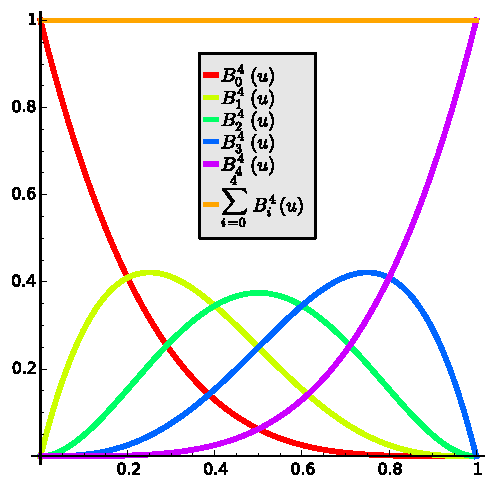
\includegraphics[width=0.6\textwidth]{images/bernstein_poly.pdf}
    \caption{Plot of Bernstein polynomial functions up to degree 4 with summation of all four functions to show characteristic of partition of one (Note the maximum of each polynomial is always at $t=\frac{i}{\textcolor{ForestGreen}{n}}$)}
    \label{fig:bernstein_poly}
\end{figure}
The polynomials relate to each other, as one can see in \autoref{eq:bernstein_polynomial_relation}.
\begin{equation}\label{eq:bernstein_polynomial_relation}
\begin{aligned}
& \frac{d}{d t} B_{i, n}(t)=n\left(B_{i-1, n-1}(t)-B_{i, n-1}(t)\right)=-n \Delta B_{i-1, n-1}(t) \\
& \frac{d^{2}}{d t^{2}} B_{i, n}(t)=n(n-1)\left(B_{i-2, n-2}(t)-2 B_{i-1, n-2}(t)+B_{i, n-2}(t)\right)=n(n-1) \Delta^{2} B_{i-2, n-2}(t) \\
& \frac{d^{k}}{d t^{k}} B_{i, n}(t)=(-1)^{k} n(n-1) \ldots(n-k+1) \Delta^{k} B_{i-k, n-k}(t)
\end{aligned}
\end{equation}
\FloatBarrier
\subsubsection{Simple Bézier Curves}
A \textcolor{Plum}{simple Bézier curve} is defined with \autoref{eq:simple_bezier_curve}. To get the idea also have a look at \autoref{fig:bezier_curve}.
\begin{equation}\label{eq:simple_bezier_curve}
\textcolor{Plum}{\vec{r}(t)}=\sum_{\textcolor{green}{i}=0}^{\textcolor{ForestGreen}{n}} \vec{P}_{\textcolor{green}{i}} B_{\textcolor{green}{i} \textcolor{ForestGreen}{n}}(t) \quad t \in[0,1]
\end{equation}
Where:
\begin{itemize}
    \item $\textcolor{green}{i}$ control point number
    \item $\textcolor{ForestGreen}{n}$ is the total number of control points minus one, since Points are ($P_0, P_1, P_2, P_n$)
\end{itemize}
\subsubsection{Composite Bézier Curves}
The simple Bézier curves meet at common control points. Which is a continuity condition ($C^0$), but often higher (smoothness) conditions are required ($C^k$-smooth). This condition is only met if and only if \autoref{eq:bezier_smooth_condition} is given.
\begin{equation} \label{eq:bezier_smooth_condition}
\frac{\Delta^{\ell} \vec{P}_{\textcolor{ForestGreen}{n}-\ell, j}}{h_j^{\ell}}=\frac{\Delta^{\ell} \vec{P}_{0, j+1}}{h_{j+1}^{\ell}} \quad(j=0,1, \cdots, m-2 \quad \ell=0,1,2, \cdots, k)
\end{equation}
Writing out \autoref{eq:bezier_smooth_condition} for $C^1$ smoothness results in \autoref{eq:bezier_smooth1}, whereas $C^2$ smoothness results in  \autoref{eq:bezier_smooth2} where one has to know that also \autoref{eq:bezier_smooth1} $C^1$ smoothness must be met.
\begin{equation}\label{eq:bezier_smooth1}
\frac{\textcolor{ForestGreen}{n}\left(\vec{P}_{\textcolor{ForestGreen}{n}, \textcolor{orange}{j}}-\vec{P}_{\textcolor{ForestGreen}{n}-1, \textcolor{orange}{j}}\right)}{h_{\textcolor{orange}{j}}}=\frac{\textcolor{ForestGreen}{n}\left(\vec{P}_{1, \textcolor{orange}{j}+1}-\vec{P}_{0, \textcolor{orange}{j}+1}\right)}{h_{\textcolor{orange}{j}+1}} \quad(\textcolor{orange}{j}=0,1, \cdots, m-2)
\end{equation}
\begin{equation}\label{eq:bezier_smooth2}
\frac{\textcolor{ForestGreen}{n}(\textcolor{ForestGreen}{n}-1)\left(\vec{P}_{\textcolor{ForestGreen}{n}, \textcolor{orange}{j}}-2 \vec{P}_{\textcolor{ForestGreen}{n}-1, \textcolor{orange}{j}}+\vec{P}_{\textcolor{ForestGreen}{n}-2, \textcolor{orange}{j}}\right)}{h_{\textcolor{orange}{j}}{ }^2}=\frac{\textcolor{ForestGreen}{n}(\textcolor{ForestGreen}{n}-1)\left(\vec{P}_{2, \textcolor{orange}{j}+1}-2 \vec{P}_{1, \textcolor{orange}{j}+1}+\vec{P}_{0, \textcolor{orange}{j}+1}\right)}{h_{\textcolor{orange}{j}+1}{ }^2} \quad(\textcolor{orange}{j}=0,1, \cdots, m-2)
\end{equation}

The Bézier-curve is defined by the control points $\left(\vec{P}_{\textcolor{green}{0}}, \vec{P}_{\textcolor{green}{1}}, \ldots \vec{P}_{\textcolor{green}{n}}(\textcolor{ForestGreen}{n} \geq 2)\right)$ and the  Bernstein polynomials. On each \textcolor{orange}{spline} one has \textcolor{ForestGreen}{n}+1 \textcolor{green}{control points}.
\begin{itemize}
    \item \textcolor{orange}{spline number}, the spline number there are m splines (m=(Number of given Data points-1))
    \item \textcolor{green}{point on spline}, there are $\textcolor{ForestGreen}{n}+1$ points on the spline
\end{itemize}
$$
\vec{r}_{\textcolor{orange}{j}}(u)=\sum_{\textcolor{green}{i}=0}^{\textcolor{ForestGreen}{n}} \vec{P}_{\textcolor{green}{i}, \textcolor{orange}{j}} B_{\textcolor{green}{i} \textcolor{ForestGreen}{n}}\left(u, u_j \cdot u_{j+1}\right) \quad u \in\left[u_j \cdot u_{j+1}\right] \quad(j=0,1, \cdots, m-1)
$$
\begin{figure}[ht!]
    \centering
    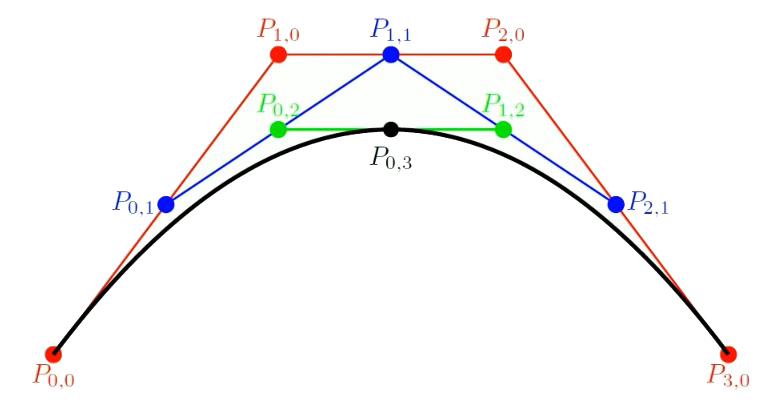
\includegraphics[width=0.8\textwidth]{images/cubic_bezier_curve.jpg}
    \caption{Cubic Bézier Curve (Always defined by 4 control points), degree three}
    \label{fig:bezier_curve}
\end{figure}
\subsubsection{Example: Composite Bézier Curves}
The four points $A=(0,0), B=(1,0), C=(2,3)$ and $D=(2,4)$ are to be interpolated (joined) by composed $C^1$ Bernstein-Bézier splines: $A$ and $B$ are to be joined  linearly (by a straight line), as well as $C$ and $D$.\newline Compute the missing $C^1$ Bernstein-Bézier spline of minimal degree between $B$ and $C$. \newline\newline
To solve the exercise one can use \autoref{eq:bezier_smooth1}. Where the first \textcolor{orange}{spline} and the last one have two control points, since it is a straight line $\Rightarrow$ $\textcolor{ForestGreen}{n}=\textcolor{violet}{1}$. The second \textcolor{orange}{spline} has four conditions, since tow points must be met and two derivatives, since it must be $C^1$ smooth. Due to that $\textcolor{ForestGreen}{n}=\textcolor{pink}{3} \Rightarrow$ the degree is also 3 (also called cubic).
$$
\begin{aligned}
    &\textcolor{violet}{1} \cdot \left(P_{\textcolor{green}{1}, \textcolor{orange}{0}}-P_{\textcolor{green}{0}, \textcolor{orange}{0}}\right)=\textcolor{pink}{3} \cdot \left(P_{\textcolor{green}{1}, \textcolor{orange}{1}}-P_{\textcolor{green}{0}, \textcolor{orange}{1}}\right)=\textcolor{violet}{1}\cdot \left(\left(\begin{array}{l} 1 \\ 0 \end{array}\right)-\left(\begin{array}{l} 0 \\ 0 \end{array}\right)\right)=\textcolor{pink}{3}\cdot\left(P_{\textcolor{green}{1}, \textcolor{orange}{1}}-\left(\begin{array}{l} 1 \\ 0 \end{array}\right)\right)\\
    & \textcolor{pink}{3} \cdot \left(P_{\textcolor{green}{3}, \textcolor{orange}{1}}-P_{\textcolor{green}{2}, \textcolor{orange}{1}}\right)=\textcolor{violet}{1}\cdot\left(P_{\textcolor{green}{1}, \textcolor{orange}{2}}-P_{\textcolor{green}{0}, \textcolor{orange}{2}}\right)=\textcolor{pink}{3}\cdot \left(\left(\begin{array}{l} 2 \\ 3 \end{array}\right)-P_{\textcolor{green}{2}, \textcolor{orange}{1}}\right)=\textcolor{violet}{1}\cdot\left(\left(\begin{array}{l} 0 \\ 0 \end{array}\right)-\left(\begin{array}{l} 1 \\ 0 \end{array}\right)\right)\\
    &\Rightarrow P_{\textcolor{green}{1}, \textcolor{orange}{1}}=\left(\begin{array}{l} \frac{4}{3} \\ 0 \end{array}\right)\\
    &\Rightarrow P_{\textcolor{green}{2}, \textcolor{orange}{1}}=\left(\begin{array}{l} 2 \\ \frac{8}{3} \end{array}\right)
\end{aligned}
$$
$$
\begin{aligned}
\vec{r}(t) & =\underbrace{P_{\textcolor{green}{0}, \textcolor{orange}{1}}}_B \cdot B_{03}(t)+P_{\textcolor{green}{1}, \textcolor{orange}{1}} \cdot B_{13}(t)+P_{\textcolor{green}{2}, \textcolor{orange}{1}} \cdot B_{23}(A)+\underbrace{P_{\textcolor{green}{0}, \textcolor{orange}{1}}}_C \cdot B_{33} \\
& =\left(\begin{array}{l}
1 \\
0
\end{array}\right)(1-t)^3+3\left(\begin{array}{l} \frac{4}{3} \\ 0 \end{array}\right)(1-t)^2 t+3\left(\begin{array}{l}
2 \\
\frac{8}{3}
\end{array}\right)(1-t) t^2+\left(\begin{array}{l}
2 \\
3
\end{array}\right) t^3
\end{aligned}
$$
$$
t \in[0,1]
$$
% \begin{wrapfigure}{R}{0.5\textwidth}
\begin{figure}[ht]
  \centering
  \resizebox{0.5\textwidth}{!}{\subimport{images/}{bezier}}
  \caption{Exercise Overview}
  \label{fig:bezier}
\end{figure}
\FloatBarrier

\subsubsection{Properties}
\begin{itemize}
    \item The Bézier-curves is always inside the convex hull of the data points.
    \item$$
    \begin{aligned}
    & \vec{r}(0)=\vec{P}_{0} \quad \vec{r}(1)=\vec{P}_{n} \\
    & \vec{r}^{\prime}(0)=n\left(\vec{P}_{1}-\vec{P}_{0}\right) \quad \vec{r}^{\prime}(1)=n\left(\vec{P}_{n}-\vec{P}_{n-1}\right) \\
    & \vec{r}^{\prime \prime}(0)=n(n-1)\left(\vec{P}_{2}-2 \vec{P}_{1}+\vec{P}_{0}\right) \quad \vec{r}^{\prime \prime}(1)=n(n-1)\left(\vec{P}_{n}-2 \vec{P}_{n-1}+\vec{P}_{n-2}\right)
    \end{aligned}
    $$
    \item If $C^{k}$ smoothness for a point is required, $k$ equations or $k$ control points are necessary
\end{itemize}
\subsubsection{Casteljau recurrence}
The Casteljau recurrence is a similar idea as the neville-aitken. With this Idea a point on the Bézier curve can be calculated as a linear combination of two points on a Bézier curve of a lower degree.
$$
\vec{r}_{\overrightarrow{P_{0}}, \overrightarrow{P_{1}}, \ldots, \overrightarrow{P_{n}}}(t)=(1-t) \cdot \vec{r}_{\overrightarrow{P_{0}}, \overrightarrow{P_{1}}, \ldots, P_{n-1}} \overrightarrow{ }(t)+t \cdot \vec{r}_{\overrightarrow{P_{1}}, \overrightarrow{P_{2}}, \ldots, \overrightarrow{P_{n}}}(t) \quad t \in[0,1]
$$

$$
\begin{array}{llll}
C^{0}: & &  P_{n}=\vec{Q}_{0} \\
C^{1}: & \vec{r}_{P}^{\prime}(1)= & n\left(\vec{P}_{n}-\vec{P}_{n-1}\right)=m\left(\vec{Q}_{1}-\vec{Q}_{0}\right) & =\vec{r}_{Q}^{\prime}(0) \\
C^{2}: & \vec{r}_{P}^{\prime \prime}(1)= & n(n-1)\left(\vec{P}_{n}-2 \vec{P}_{n-1}+\vec{P}_{n-2}\right)=m(m-1)\left(\vec{Q}_{2}-2 \vec{Q}_{1}+\vec{Q}_{0}\right) & =\vec{r}_{Q}^{\prime \prime}(0) \\
C^{k}: & \vec{r}_{P}^{(k)}(1)= & n(n-1) \ldots(n-k+1)\left(\Delta^{k} \vec{P}_{n-k}\right)=m(m-1) \ldots(m-k+1)\left(\Delta^{k} \vec{Q}_{0}\right) & =\vec{r}_{Q}^{(k)}(0)
\end{array}
$$
Is $\overrightarrow{r_{j}}(t)=\sum_{i=0}^{n} \vec{P}_{i, j} B_{i, n}(t) \quad t \in[0,1]$ with the functions $Q_{j}$ defined (degree: $n$ ), the following formulas turn out:
$$
\begin{array}{llll}
C^{0}: & \vec{P}_{n, j-1}=\vec{P}_{0, j}=\vec{Q}_{j} \\
C^{1}: & \vec{r}_{j-1}^{\prime}(1)= & \vec{Q}_{j}-\vec{P}_{n-1, j-1}=\vec{P}_{1, j}-\vec{Q}_{j} & =\vec{r}_{j}^{\prime}(0) \\
C^{2}: & \vec{r}_{j-1}^{\prime \prime}(1)= & \vec{Q}_{j}-2 \vec{P}_{n-1, j-1}+\vec{P}_{n-2, j-1}=\vec{P}_{2, j}-2 \vec{P}_{1, j}+\vec{Q}_{j} & =\vec{r}_{j}^{\prime \prime}(0) \\
C^{k}: & \vec{r}_{j-1}^{(k)}(1)= & \Delta^{k} \vec{P}_{n-k, j-1}=\Delta^{k} \vec{P}_{0, j} & =\vec{r}_{j}^{(k)}(0)
\end{array}
$$





\subsubsection{Example}
Let's do the same example as in \autoref{subsubsec:ex_spline}. Where the following four points are given: 
$$\left\{\underbrace{(0,0)}_{Q_0=P_{\textcolor{green}{0}, \textcolor{orange}{0}}},\underbrace{\left(\frac{\pi}{3}, \frac{\sqrt{3}}{2}\right)}_{Q_1=P_{\textcolor{green}{0}, \textcolor{orange}{1}}=P_{\textcolor{green}{3}, \textcolor{orange}{0}}},\left(\frac{2 \pi}{3}, \frac{\sqrt{3}}{2}\right),(\pi, 0)\right\}$$
Therefore $\vec{Q}_0=(0,0), \vec{Q}_1=\left(\frac{\pi}{3}, \frac{\sqrt{3}}{2}\right), \dots$ and $h_j=h=\frac{\pi}{3}$. One now has to met the following requirements: 

$$
\begin{aligned}
&\vec{Q}_1-\vec{P}_{\textcolor{green}{2},\textcolor{orange}{0}}=\vec{P}_{\textcolor{green}{1},\textcolor{orange}{1}}-\vec{Q}_1 \\
&\vec{Q}_2-\vec{P}_{2,1}=\vec{P}_{1,2}-\vec{Q}_2 \\
&\vec{Q}_1-2 \vec{P}_{2,0}+\vec{P}_{1,0}=\vec{P}_{2,1}-2 \vec{P}_{1,1}+\vec{Q}_1 \\
&\vec{Q}_2-2 \vec{P}_{2,1}+\vec{P}_{1,1}=\vec{P}_{2,2}-2 \vec{P}_{1,2}+\vec{Q}_2
\end{aligned}
$$

$$
\begin{aligned}
&\vec{P}_{2,0}-2 \vec{P}_{1,0}+\vec{Q}_0=\overrightarrow{0} \\
&\vec{Q}_3-2 \vec{P}_{2,2}+\vec{P}_{1,2}=\overrightarrow{0}
\end{aligned}
$$

The solution of the linear system above gives us the following points:
$$
\left\{\underbrace{\left\{\frac{\pi}{9}, \frac{\sqrt{3}}{5}\right\}}_{P_{\textcolor{green}{1}, \textcolor{orange}{0}}},\underbrace{\left\{\frac{2 \pi}{9}, \frac{2 \sqrt{3}}{5}\right\}}_{P_{\textcolor{green}{2}, \textcolor{orange}{0}}},\underbrace{\left\{\frac{4 \pi}{9}, \frac{3 \sqrt{3}}{5}\right\}}_{P_{\textcolor{green}{1}, \textcolor{orange}{1}}},\underbrace{\left\{\frac{5 \pi}{9}, \frac{3 \sqrt{3}}{5}\right\}}_{P_{\textcolor{green}{2}, \textcolor{orange}{1}}},\left\{\frac{7 \pi}{9}, \frac{2 \sqrt{3}}{5}\right\},\left\{\frac{8 \pi}{9}, \frac{\sqrt{3}}{5}\right\}\right\}
$$

When we now calculate the first spline we get the same result as before.
\begin{equation}
\begin{aligned}
\vec{r_1}(t)&=\left(\begin{array}{c}
\frac{1}{9} \pi \mathrm{B}_{1,3}(t)+\frac{2}{9} \pi \mathrm{B}_{2,3}(t)+\frac{1}{3} \pi \mathrm{B}_{3,3}(t) \\
\frac{1}{5} \sqrt{3} \mathrm{~B}_{1,3}(t)+\frac{2}{5} \sqrt{3} \mathrm{~B}_{2,3}(t)+\frac{1}{2} \sqrt{3} \mathrm{~B}_{3,3}(t)
\end{array}\right)\\
&=\left(\begin{array}{l}
\frac{\pi}{9} 3(1-t)^2 t+\frac{2 \pi}{9} 3(1-t) t^2+\frac{1}{3} \pi t^3 \\
\frac{\sqrt{3}}{5} 3(1-t)^2 t+\frac{2}{5} \sqrt{3} 3(1-t) t^2+\frac{\sqrt{3}}{2} t^3
\end{array}\right)\\
&=\left(\begin{array}{l}
x \\
y
\end{array}\right)\\
\Longleftrightarrow & \left(\begin{array}{c}
\frac{\pi}{3} t=x \\
\frac{3 \sqrt{3}}{5} t-\frac{\sqrt{3}}{10} t^3=y
\end{array}\right) \Rightarrow\left(\begin{array}{l}
t=\frac{3 x}{\pi} \\
y=\frac{9 \sqrt{3}}{5 \pi} x-\frac{27 \sqrt{3}}{10 \pi^3} x
\end{array}\right)
\end{aligned}
\end{equation}
For the second spline we get the following:
\begin{equation}
\left(\begin{array}{c}
\frac{1}{3} \pi \mathrm{B}_{0,3}(t)+\frac{4}{9} \pi \mathrm{B}_{1,3}(t)+\frac{5}{9} \pi \mathrm{B}_{2,3}(t)+\frac{2}{3} \pi \mathrm{B}_{3,3}(t) \\
\frac{1}{2} \sqrt{3} \mathrm{~B}_{0,3}(t)+\frac{3}{5} \sqrt{3} \mathrm{~B}_{1,3}(t)+\frac{3}{5} \sqrt{3} \mathrm{~B}_{2,3}(t)+\frac{1}{2} \sqrt{3} \mathrm{~B}_{3,3}(t)
\end{array}\right)
\end{equation}

\section{Linear Least-Squares approximation}
\subsection{Idea}
Interpolation with the collocation methods often run into oscillation problems for (rather large) sets of measurement points. Furthermore, in most cases the measurements also contain some error points, which one does not want to represent in the graph. Due to that, an approximation (data points are not represented exactly any more) might be the preferred way to represent the data. 
\subsection{Linear Least-Squares}
To find the best approximation, one must define what is a good and what is a bad approximation, which could be with the following basic functions:\newline
$$
\begin{aligned}
    \Rightarrow \text{Basics of functions} & \Rightarrow min(max\mid r_i \mid)\\
    & \Rightarrow \sum_{i \dots} \mid r_i \mid\\
    & \Rightarrow \sum_{i \dots}  r_i^2\\
\end{aligned}
$$
Note: Error = residuals $\Rightarrow$ norm of residuals\newline
Mathematically, the minimization of the squared errors is the easiest, therefore this one is most commonly used (least square approximation)
\begin{wrapfigure}{r}{0.5\textwidth}
  \centering
  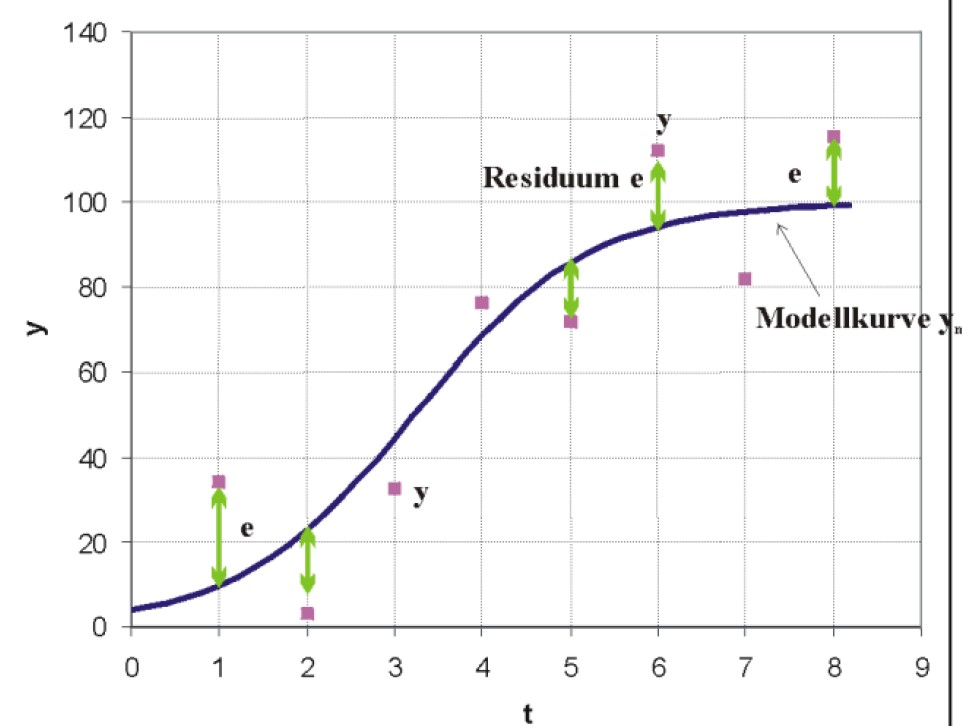
\includegraphics[width=0.45\textwidth]{images/Screenshot 2022-10-26 091954.jpg}
  \caption{Data approximated by an error curve}
  \label{fig:overview}
\end{wrapfigure}\newline
The approximation function can be described with a set of basis functions, which we name here $g_0, g_1, \ldots, g_m=\left\{g_j\right\}_{j=0, \ldots, m}$. Note the basis functions are sometimes also called  monomials.
Furthermore we define the following
\begin{itemize}
    \item N: Number of sample points
    \item m: degree of basic functions (m $\ll$ N)
    \item a: weighting coefficients
    \item $\left(x_0, y_0\right),\left(x_1, y_1\right)_1, \ldots,\left(x_N, y_N\right)=\left\{\left(x_i, y_i\right)\right\}_{i=0, \ldots, N}$: measurement points
\end{itemize}
With those variables one can create a equation in matrix notation form, as can be seen in \autoref{eq:leas_square_design_matrix}:

\begin{equation}\label{eq:leas_square_design_matrix}
\overbrace{\left(\begin{array}{cccc}
g_{0}\left(x_{0}\right) & g_{1}\left(x_{0}\right) & \ldots & g_{m}\left(x_{0}\right) \\
\vdots & \vdots & \ddots & \vdots \\
\vdots & \vdots & \ddots & \vdots \\
g_{0}\left(x_{N}\right) & g_{1}\left(x_{N}\right) & \ldots & g_{m}\left(x_{N}\right)
\end{array}\right)}^{\text {Designmatrix } G} \cdot\left(\begin{array}{c}
a_{0} \\
\vdots \\
a_{m}
\end{array}\right)=\left(\begin{array}{c}
y_{0} \\
\vdots \\
\vdots \\
y_{N}
\end{array}\right) \Leftrightarrow \quad G \cdot a=y
\end{equation}
Since \autoref{eq:leas_square_design_matrix} is normally overdetermined (m$\ll$N) The error/residuals can be calculated with \autoref{eq:least_square} and the squared sum S of residuals with \autoref{eq:least_square_squared}. The goal is now to minimize S from \autoref{eq:least_square_squared}. This can be done with \autoref{eq:least_square_g}, which is not derived in this post (for more information, search after orthogonal projection).



\begin{equation}\label{eq:least_square}
r_i=y_i-\sum_{j=0}^m a_j g_j\left(x_i\right) \quad(i=0, \ldots, N)
\end{equation}
\begin{equation} \label{eq:least_square_squared}
\underbrace{S}_{\text{Error}}=\sum_{i=0}^N\left(y_i-\underbrace{\sum_{j=0}^m a_j g_j\left(x_i\right)}_{\text{Model}}\right)^2=\sum_{i=0}^N r_i^2 \Rightarrow \min !
\end{equation}
\subsubsection{Thinking hint}
Lets assume one has the following points: $\{1,1\},\{2,2\}$ and one wants to approximate those points by a polynomial of degree zero ($m=0$) $\Rightarrow g_0(x)=1$. Then one can write the term inside the square brackets as the following:
$$
\overbrace{\left[\begin{array}{c}
1 \\
2 \\
\end{array}\right]}^{y}-
\overbrace{\left[\begin{array}{c}
1\\
1
\end{array}\right]}^{\textbf{G}} \cdot
\overbrace{\left[\begin{array}{c}
a
\end{array}\right]}^{a}
$$
But as one can see one can not take the square of this term, therefore one has to multiply on both left sides with $\textbf{G}^T$ which has no effect on the end result, since one is only interested in the minimum.
$$
\overbrace{\left[\begin{array}{cc}
1 & 1\\
\end{array}\right]}^{\textbf{$G^T$}} \cdot
\overbrace{\left[\begin{array}{c}
1 \\
2 \\
\end{array}\right]}^{y}-
\overbrace{\left[\begin{array}{cc}
1 &1
\end{array}\right]}^{\textbf{$G^T$}} \cdot
\overbrace{\left[\begin{array}{c}
1\\
1
\end{array}\right]}^{\textbf{G}} \cdot
\overbrace{\left[\begin{array}{c}
a
\end{array}\right]}^{a}
$$
When one squares the term above and says that $\textbf{G}^T\cdot y$ and $\textbf{G}^T\cdot \textbf{G}$ belong to each other, (are not separable) and then takes furthermore the derivative, one gets the following result: $2\cdot \left(a\cdot (\textbf{G}^T\cdot \textbf{G})-(\textbf{G}^T\cdot y)  \right)\cdot (\textbf{G}^T\cdot \textbf{G})$. When one sets this term to zero since one is interested in the minimum and solves it after $a$ one gets the result from \autoref{eq:least_square_g}.
\subsubsection{Normal equations}
\begin{equation}\label{eq:least_square_g}
\underbrace{\boldsymbol{G}^{T} \boldsymbol{G}}_{\text {Normal matrix }} \cdot \boldsymbol{a}=\boldsymbol{G}^{T} \boldsymbol{y} \quad \Rightarrow \quad \boldsymbol{a}=\left(\boldsymbol{G}^{T} \boldsymbol{G}\right)^{-1} \boldsymbol{G}^{T} \boldsymbol{y}
\end{equation}
$$
\begin{aligned}
& \underbrace{\underbrace{\boldsymbol{G}^{T}}_{(m+1) \times(N+1)}}_{(m+1) \times(m+1)} \cdot \underbrace{\boldsymbol{G}}_{(N+1) \times(m+1)} \cdot \underbrace{\boldsymbol{a}}_{(m+1) \times 1}=\underbrace{\boldsymbol{G}^{T}}_{(m+1) \times 1} \cdot \underbrace{\boldsymbol{y}}_{(N+1) \times 1}
\end{aligned}
$$
\subsection{Singular-value decomposition (SVD)}
A \href{https://en.wikipedia.org/wiki/Singular_value_decomposition}{singular-value decomposition} is one of the most widely used matrix operations in applied linear algebra.
\subsubsection{Idea}
Every Matrix $\boldsymbol{G}$ with the dimensions $(N+1) \times(m+1)$ can be decomposed as the triple product $\boldsymbol{U} \boldsymbol{D} \boldsymbol{V}^{T}$ whereas $\boldsymbol{U}$ is an \href{https://en.wikipedia.org/wiki/Orthogonal_matrix}{orthogonal} (N +1) × (N +1) -matrix, $\boldsymbol{D}$ is a (N +1) × (m +1) diagonal matrix and $\boldsymbol{V}$ again is orthogonal with dimensions (m +1) × (m +1). When a matrix is orthogonal, the following applies: $Q^{\mathrm{T}} Q=Q Q^{\mathrm{T}}=I$ and $Q^{\mathrm{T}}=Q^{-1}$. Due to that nice property, \autoref{eq:leas_square_design_matrix} can be calculated according to \autoref{eq:singular_value_decomposition_2}.
\begin{equation}\label{eq:singular_value_decomposition}
\boldsymbol{G}=\boldsymbol{U} \boldsymbol{D} \boldsymbol{V}^{T}=\boldsymbol{U} \cdot\left[\begin{array}{cccc}
d_{00} & 0 & \ldots & 0 \\
0 & d_{11} & \ldots & 0 \\
\vdots & \vdots & \ddots & 0 \\
0 & \ldots & 0 & d_{m m} \\
0 & 0 & \ldots & 0 \\
\vdots & \vdots & \ddots & 0 \\
0 & 0 & \ldots & 0
\end{array}\right] \cdot \boldsymbol{V}^{T}
\end{equation}


$G a_|=y_|$ becomes $U D V^{T} a_|=y_|$. Which results in \autoref{eq:singular_value_decomposition_2}
\begin{equation}\label{eq:singular_value_decomposition_2}
a_|=V D^{-1} U^{T} \cdot y_|
\end{equation}
% \subsubsection{Exercise one}

% \paragraph{Design matrix G}
% G: $(N+1)\cdot(m+1)$


% \begin{equation}
% \begin{array}{l|l|l|l|l|l} 
% & g_0 & g_1 & g_2 & \cdots & g_m \\
% \hline 
% x_0 & g_0\left(x_0\right) & g_1\left(x_0\right) &&\\
% x_1 & g_0\left(x_1\right) & g_1\left(x_1\right) && \\
% x_2 & \vdots & \vdots &&&\\
% x_N & g_0\left(x_N\right) & g_1\left(x_N\right) &&
% \end{array}
% \end{equation}
% With \autoref{eq:least_square} we can crete the following matrix


\subsubsection{Uniform arguments and orthogonal polynomials}
With uniform arguments $x_{i}-x_{j}=(j-i) h$ for all  $i, j \rightarrow\left\{x_{0} \ldots x_{N}\right\}=\left\{x_{0}+t \cdot h\right\}_{t=0 \ldots N}$ and orthogonal polynomials $G G^{T}$ can be diagonalized and therefore the equation can be easier solved. An example can be found in \autoref{subsubsec:orthognal_example}

\begin{equation}\label{eq:orthogonal_polynomials}
    \begin{aligned}
    p_{k, N}(t)&=\sum_{i=0}^{k}(-1)^{i}\left(\begin{array}{c}
    k \\
    i
    \end{array}\right)\left(\begin{array}{c}
    k+i \\
    i
    \end{array}\right) \frac{t^{(i)}}{N^{(i)}}\\&=1+\sum_{i=1}^{k}(-1)^{i}\left(\begin{array}{c}
    k \\
    i
    \end{array}\right)\left(\begin{array}{c}
    k+i \\
    i
    \end{array}\right) \frac{t(t-1)(t-2) \ldots(t-i+1)}{N(N-1)(N-2) \ldots(N-i+1)} \quad(k=1, \ldots, N)
    \end{aligned}
\end{equation}


with $t=\frac{x-x_{0}}{h} \quad\left(\begin{array}{l}k \\ i\end{array}\right)=\frac{k !}{i !(k-i) !}=n C r(k, i)$

$p_{k, N}$ can now with $g_{k}$ be put in the design matrix and the product $G^{T} G$ will be a $(m+1) \times(m+1)$ Diagonal matrix. Afterwards $a$ can be calculated with the knows formula $G^{T} G a=G^{T} y$.

\subsubsection{Calculation of the first terms for orthogonal polynomials:}\label{subsubsec:calc_orthog}
From \autoref{eq:orthogonal_polynomials} one knows that $N^{(i)}$ and $t^{(i)}$ are the following:
\begin{equation}
N^{(i)}=\underbrace{\underbrace{(N-1)}_{N^0}(N-2)}_{N^1}(N-2) \cdots(N-i+1)
\end{equation}
\begin{equation}
t^{(i)}=\underbrace{\underbrace{(t-0)}_{t^1}(t-1)}_{t^1}(t-2) \cdots(t-i+1)
\end{equation}


$$
p_{0, 4}(t)=\sum_{i=0}^0(-1)^0\left(\begin{array}{c}
0 \\
0
\end{array}\right)\left(\begin{array}{c}
0+0 \\
0
\end{array}\right) \frac{1\textcolor{gray}{=t^{0}}}{1=\textcolor{gray}{4^0}} =\underline{\underline{1}}
$$

$$
\begin{aligned}
p_{1, 4}(t)&=\sum_{i=0}^1(-1)^i\left(\begin{array}{c}
1 \\
i
\end{array}\right)\left(\begin{array}{c}
1+i \\
i
\end{array}\right) \frac{t^{i}}{N^{i}} \\
&=(-1)^0\underbrace{\left(\begin{array}{c}
1 \\
0
\end{array}\right)}_{=1}\underbrace{\left(\begin{array}{c}
1+0 \\
0
\end{array}\right)}_{=1} \frac{1\textcolor{gray}{=t^{(0)}}}{1=\textcolor{gray}{4^0}}\\&+
(-1)^1\underbrace{\left(\begin{array}{c}
1 \\
1
\end{array}\right)}_{=1}\underbrace{\left(\begin{array}{c}
1+1 \\
1
\end{array}\right)}_{=2} \frac{t\textcolor{gray}{=t^{(1)}}}{4=\textcolor{gray}{4^1}}\\ &=\underline{\underline{1-\frac{t}{2}}}
\end{aligned}
$$

$$
\begin{aligned}
p_{2, 4}(t)&=\sum_{i=0}^2(-1)^i\left(\begin{array}{c}
2 \\
i
\end{array}\right)\left(\begin{array}{c}
2+i \\
i
\end{array}\right) \frac{t^{i}}{N^{i}} \\
&=(-1)^0\underbrace{\left(\begin{array}{c}
2 \\
0
\end{array}\right)}_{=1}\underbrace{\left(\begin{array}{c}
2+0 \\
0
\end{array}\right)}_{=1} \frac{1\textcolor{gray}{=t^{(0)}}}{1=\textcolor{gray}{4^0}}\\&+
(-1)^1\underbrace{\left(\begin{array}{c}
2 \\
1
\end{array}\right)}_{=2}\underbrace{\left(\begin{array}{c}
2+1 \\
1
\end{array}\right)}_{=3} \frac{t\textcolor{gray}{=t^{(1)}}}{4=\textcolor{gray}{4-0}}\\&+
(-1)^2\overbrace{\left(\begin{array}{c}
2 \\
2
\end{array}\right)}^{=\frac{2 !}{2 !(2-2) !}=1}\underbrace{\left(\begin{array}{c}
2+2 \\
2
\end{array}\right)}_{=\frac{4 !}{2 !(4-2) !}=6} \frac{t\cdot(t-1)\textcolor{gray}{=t^2-t}}{4 \cdot (4-1)=\textcolor{gray}{12}}\\ &=\underline{\underline{1-\frac{3}{2}\cdot t+\frac{1}{2}\cdot t^2-\frac{1}{2}\cdot t}}
\end{aligned}
$$












% \subsubsection{Example:}

% $$
% \boldsymbol{x}=\left[\begin{array}{lllll}
% 3 & 4 & 5 & 6 & 7
% \end{array}\right] \quad \Rightarrow \quad \boldsymbol{t}=\boldsymbol{x}-3=\left[\begin{array}{lllll}
% 0 & 1 & 2 & 3 & 4
% \end{array}\right]
% $$

% $\Rightarrow P_{0}(x)=1 \quad P_{1}(x)=1-\frac{x-3}{2} \quad P_{2}(x)=1-\frac{2 \cdot 3(x-3)}{4}+\frac{1 \cdot 3(x-3)(x-3-1)}{4 \cdot 3}=1-\frac{3 x-9}{2}+\frac{1}{2}(x-4)(x-3) ? ? ?$

% $$
% \boldsymbol{G}=\left[\begin{array}{ccc}
% P_{0} & P_{1} & P_{2} \\
% 1 & 1 & 1 \\
% 1 & 1 / 2 & -1 / 2 \\
% 1 & 0 & -1 \\
% 1 & -1 / 2 & -1 / 2 \\
% 1 & -1 & 1
% \end{array}\right] \quad \Rightarrow \quad \boldsymbol{G}^{T} \boldsymbol{G}=\left[\begin{array}{ccc}
% \left\|P_{0}\right\|^{2} & 0 & 0 \\
% 0 & \left\|P_{1}\right\|^{2} & 0 \\
% 0 & 0 & \left\|P_{2}\right\|^{2}
% \end{array}\right]=\left[\begin{array}{ccc}
% 5 & 0 & 0 \\
% 0 & \frac{5}{2} & 0 \\
% 0 & 0 & \frac{7}{2}
% \end{array}\right]
% $$


\subsubsection{Exercise one, least square parabola}\label{subsubsec:least_square_ex1}
Compute a linear least-squares approximating parabola for the "second window" of five consecutive points (starting with x = 2) in the data.
$$
\begin{aligned}
\{\{x, y\}\}=&\{\{1,1.04\},\{2,1.37\},\{3,1.70\},\{4,2.00\},\{5,2.26\}\\
&\{6,2.42\},\{7,2.70\},\{8,2.78\},\{9,3.00\},\{10,3.14\}\}
\end{aligned}
$$
Lets also say the following:
\begin{itemize}
    \item m = deg = 2 (polys)  $\{1;x;x^2\}$
    \item N=4 (number of arguments actually 5 points)
\end{itemize}
Note: Normally: m$\ll$N (The degree is smaller than the number of points)
\paragraph{Write down the design matrix and the system of normal equations.}
$$
G=
\left\{\begin{array}{c|ccc}
 & g_0 & g_1 & g_2 \\
\hline 
x_0 & g_0\left(x_0\right) & g_1\left(x_0\right) & g_2\left(x_0\right) \\
x_1 & g_0\left(x_1\right) & g_1\left(x_1\right) & g_2\left(x_1\right)\\
x_2 &\vdots&\vdots&\vdots \\
x_3 &  \\
x_4 &  
\end{array}\right\}
=
\left\{\begin{array}{c|ccc}
 & 1 & x & x^2 \\
\hline 
2 & 1 & 2 & 4 \\
3 & 1 & 3 & 9 \\
4 & 1 & 4 & 16 \\
5 & 1 & 5 & 25 \\
6 & 1 & 6 & 36 
\end{array}\right\}
$$
\begin{equation}
\overbrace{\left(\begin{array}{ccc}
1 & 2 & 4 \\
1 & 3 & 9 \\
1 & 4 & 16 \\
1 & 5 & 25 \\
1 & 6 & 36 
\end{array}\right)}^{\text{Design matrix G}} \cdot\left(\begin{array}{l}
a_0 \\
a_1 \\
a_2
\end{array}\right)=\left(\begin{array}{l}
1.37 \\
1.70 \\
2.00 \\
2.26 \\
2.42 
\end{array}\right)
\end{equation}
With  \autoref{eq:least_square_g} we get the system of normal equations as one can see in \autoref{eq:least_squre_system_of_normal_equations}:
$$
\overbrace{\left[\begin{array}{ccccc}
1 & 1 & 1 & 1 & 1 \\
2 & 3 & 4 & 5 & 6 \\
4 & 9 & 16 & 25 & 36
\end{array}\right]}^{\textbf{G}^T} \cdot \overbrace{\left[\begin{array}{c}
1.37 \\
1.7 \\
2 \\
2.26 \\
2.42
\end{array}\right]}^{y} =\left[\begin{array}{c}
9.75 \\
41.66 \\
196.4
\end{array}\right]
$$
$$
\overbrace{\left[\begin{array}{ccccc}
1 & 1 & 1 & 1 & 1 \\
2 & 3 & 4 & 5 & 6 \\
4 & 9 & 16 & 25 & 36
\end{array}\right]}^{G^{T}G} \cdot \overbrace{\left[\begin{array}{ccc}
1 & 2 & 4 \\
1 & 3 & 9 \\
1 & 4 & 16 \\
1 & 5 & 25 \\
1 & 6 & 36
\end{array}\right]}^G=
\left[\begin{array}{ccc}
5 & 20 & 90 \\
20 & 90 & 440 \\
90 & 440 & 2274
\end{array}\right]
$$
\begin{equation}\label{eq:least_squre_system_of_normal_equations}
\overbrace{\left(\begin{array}{ccc}
5 & 20 & 90 \\
20 & 90 & 440 \\
90 & 440 & 2274
\end{array}\right)}^{G^{T}G} \cdot\left(\begin{array}{l}
a_0 \\
a_1 \\
a_2
\end{array}\right)=\left(\begin{array}{c}
9.75 \\
41.66 \\
196.4
\end{array}\right)
\end{equation}
\paragraph{Solve the linear system}
$$
\begin{aligned}
&a_0=0.506 ; a_1=0.483143 ; a_2=-0.0271429 \\
&y=a_0 \cdot 1+a_1 \cdot x+a_2\cdot x^2
\end{aligned}
$$
When one wants to increase the stability of the matrix one can make a statistical normalization.
\paragraph{Compute the output y and the derivative (!) of the approximation at the central coordinate (x = 4)} \label{par:result1}
$$
y(4)=\underline{\underline{2.00429}} ; \quad y^{\prime}(4)=a_1+2 a_2 \cdot 4=\underline{\underline{0.266}}
$$
\subsubsection{Excercise three, Savitzky Golay filter}
Apply the filter formulas developed in the exercise before for the data to compute approximately y for $x = 3, \dots , 8$
$$
\begin{array}{|l|cccccccccc|}
\hline \boldsymbol{x}_{\boldsymbol{k}} & \mathbf{1} & \mathbf{2} & \mathbf{3} & \mathbf{4} & \mathbf{5} & \mathbf{6} & \mathbf{7} & \mathbf{8} & \mathbf{9} & \mathbf{1 0} \\
\hline y_k & 1.04 & 1.37 & 1.70 & 2.00 & 2.26 & 2.42 & 2.70 & 2.78 & 3.00 & 3.14 \\
\hline
\end{array}
$$

$$
\begin{aligned}
&k=2 \Rightarrow x=3: a_0=y_2-\frac{3}{35} \Delta^4 y_0=1.7 c-\frac{3}{35} 0.02=1.6983 \\
&k=3 \Rightarrow x=4: a_0=y_3-\frac{3}{35} \Delta^4 y_1=2-\frac{3}{35}(-0.05)=2.0043 \\
&k=4 \Rightarrow x=5: a_0=y_4-\frac{3}{35} \Delta^4 y_2=2.26-\frac{3}{35}(0.28)=2.236 \\
&k=5 \Rightarrow x=6: a_0=y_5-\frac{3}{35} \Delta^4 y_3=2.42-\frac{3}{35}(-0.54)=2.4663 \\
&k=6 \Rightarrow x=7: a_0=y_6-\frac{3}{35} \Delta^4 y_4=2.7-\frac{3}{35}(0.66)=2.6434 \\
&k=7 \Rightarrow x=8: a_0=y_7-\frac{3}{35} \Delta^4 y_5=2.78-\frac{3}{35}(-0.56)=2.828
\end{aligned}
$$
\subsubsection{Exercise four, orthogonal polynomials}\label{subsubsec:orthognal_example}
Solve \autoref{subsubsec:least_square_ex1} again by using the orthogonal polynomials $\left\{p_{k, N}(t)\right\}_{k=0, \ldots, 2}$\newline
From \autoref{eq:orthogonal_polynomials} and \autoref{subsubsec:calc_orthog} one knows the three basis functions:
$$
P_{0,4}(t)=1=g_0 ; \quad P_{1,4}(t)=1-\frac{1}{2}t=g_1(t) ; \quad P_{2,4}(t)=1-2\cdot t +\frac{1}{2}t^2=g_2(t)
$$
Now we fist have to find a transformation. The transformation can be written in  the follwoing way:
$$
t=\frac{x-2}{1}=x-2 \in\{0, \cdots, 4\}
$$
$$
G=
\left\{\begin{array}{c|ccc}
 & g_0 & g_1 & g_2 \\
\hline 
t_0 & g_0\left(t_0\right) & g_1\left(t_0\right) & g_2\left(t_0\right) \\
t_1 & g_0\left(t_1\right) & g_1\left(t_1\right) & g_2\left(t_1\right)\\
t_2 &\vdots&\vdots&\vdots \\
t_3 &  \\
t_4 &  
\end{array}\right\}
=
\left\{\begin{array}{c|ccc}
 & 1 & 1-\frac{1}{2}t & 1-2\cdot t +\frac{1}{2}t^2 \\
\hline 
0 & 1 & 1 & 1 \\
1 & 1 & \frac{1}{2} & -\frac{1}{2} \\
2 & 1 & 0 & -1 \\
3 & 1 & -\frac{1}{2} & -\frac{1}{2} \\
4 & 1 & -1 & 1 
\end{array}\right\}
$$
\begin{equation}
\overbrace{\left(\begin{array}{ccc}
1 & 1 & 1 \\
1 & \frac{1}{2} & -\frac{1}{2} \\
1 & 0 & -1 \\
1 & -\frac{1}{2} & -\frac{1}{2} \\
1 & -1 & 1 
\end{array}\right)}^{\text{Design matrix G}} \cdot\left(\begin{array}{l}
a_0 \\
a_1 \\
a_2
\end{array}\right)=\left(\begin{array}{l}
1.37 \\
1.70 \\
2.00 \\
2.26 \\
2.42 
\end{array}\right)
\end{equation}
With  \autoref{eq:least_square_g} we get the system of normal equations as one can see in \autoref{eq:least_squre_system_of_normal_equations_ex4}:
$$
\overbrace{\left[\begin{array}{ccccc}
1 & 1 & 1 & 1 & 1 \\
1 & \frac{1}{2} & 0 & -\frac{1}{2} & -1 \\
1 & -\frac{1}{2} & -1 & -\frac{1}{2} & 1
\end{array}\right]}^{\textbf{G}^T} \cdot \overbrace{\left[\begin{array}{c}
1.37 \\
1.7 \\
2 \\
2.26 \\
2.42
\end{array}\right]}^{y} =\left[\begin{array}{c}
9.75 \\
-1.33 \\
-0.19
\end{array}\right]
$$
$$
\overbrace{\left[\begin{array}{ccccc}
1 & 1 & 1 & 1 & 1 \\
1 & \frac{1}{2} & 0 & -\frac{1}{2} & -1 \\
1 & -\frac{1}{2} & -1 & -\frac{1}{2} & 1
\end{array}\right]}^{G^{T}G} \cdot \overbrace{\left[\begin{array}{ccc}
1 & 1 & 1 \\
1 & \frac{1}{2} & -\frac{1}{2} \\
1 & 0 & -1 \\
1 & -\frac{1}{2} & -\frac{1}{2} \\
1 & -1 & 1 
\end{array}\right]}^G=
\left[\begin{array}{ccc}
5 & 0 & 0 \\
0 & \frac{5}{2} & 0 \\
0 & 0 & \frac{7}{2}
\end{array}\right]
$$
\begin{equation}\label{eq:least_squre_system_of_normal_equations_ex4}
\overbrace{\left(\begin{array}{ccc}
5 & 0 & 0 \\
0 & \frac{5}{2} & 0 \\
0 & 0 & \frac{7}{2}
\end{array}\right)}^{G^{T}G} \cdot\left(\begin{array}{l}
a_0 \\
a_1 \\
a_2
\end{array}\right)=\overbrace{\left(\begin{array}{c}
9.75 \\
-1.33 \\
-0.19
\end{array}\right)}^{y}
\end{equation}
When we now calculate $(G^{T}G)^{-1}\cdot y$ one gets $\left(\begin{array}{c}
1.95 \\
-0.532 \\
-\frac{0.38}{7}
\end{array}\right)$
The result is therefore:
$$
\begin{aligned}
&y(x)=a_0 \cdot 1+a_1 \cdot p_{1,4}(t)+a_2 \cdot p_{2,4}(x)\\
&y(x=4)=y(t=2)=a_0+a_1 \cdot 0+a_2(-1)=\underline{\underline{2,00429}}\\
&\begin{aligned}
y^{\prime}(x=4)&=\frac{1}{1} y^{\prime}(x=2)=a_1 p_{1,4}^{\prime}(2)+a_2 p_{2,4}^{\prime}(2).\\
&=a_1\left(-\frac{1}{2}\right)+\left(-2+2\right)=\underline{\underline{0.266}}
\end{aligned}
\end{aligned}
$$
Which is the same as in\autoref{par:result1}.







\subsubsection{Exercise five, singular value decomposition}
Examine and compute a least-squares approximative quadratic parabola for the data
$$
\begin{array}{|l|l|l|l|l|l|}
\hline x & -2 & -1 & 0 & 1 & 2 \\
\hline y & 0 & 1 & 2 & 3 & 1 \\
\hline
\end{array}
$$
with respect to the basis functions $\left\{1,-\frac{x}{2}, \frac{x^2}{2}-1\right\}$ in the following sense:
\paragraph{Compute the design matrix G and the normal matrix. Hint: The normal matrix here is diagonal!}
$$
G=
\left\{\begin{array}{c|ccc}
 & g_0 & g_1 & g_2 \\
\hline 
x_0 & g_0\left(x_0\right) & g_1\left(x_0\right) & g_2\left(x_0\right) \\
x_1 & g_0\left(x_1\right) & g_1\left(x_1\right) & g_2\left(x_1\right)\\
x_2 &\vdots&\vdots&\vdots \\
x_3 &  \\
x_4 &  
\end{array}\right\}
=
\left\{\begin{array}{c|ccc}
 & 1 & -\frac{x}{2} & \frac{x^2}{2}-1 \\
\hline 
-2 & 1 & 1 & 1 \\
-1 & 1 & \frac{1}{2} & -\frac{1}{2} \\
0 & 1 & 0 & -1 \\
1 & 1 & -\frac{1}{2} & -\frac{1}{2} \\
2 & 1 & -1 & 1 
\end{array}\right\}
$$

\begin{equation}
\overbrace{\left(\begin{array}{ccc}
1 & 1 & 1 \\
1 & \frac{1}{2} & -\frac{1}{2} \\
1 & 0 & -1 \\
1 & -\frac{1}{2} & -\frac{1}{2} \\
1 & -1 & 1 
\end{array}\right)}^{\text{Design matrix G}} \cdot\left(\begin{array}{l}
a_0 \\
a_1 \\
a_2
\end{array}\right)=\left(\begin{array}{l}
0 \\
1 \\
2 \\
3 \\
1 
\end{array}\right)
\end{equation}
$$
\overbrace{\left[\begin{array}{ccccc}
1 & 1 & 1 & 1 & 1 \\
1 & \frac{1}{2} & 0 & -\frac{1}{2} & -1 \\
1 & -\frac{1}{2} & -1 & -\frac{1}{2} & 1
\end{array}\right]}^{\textbf{G}^T} \cdot \overbrace{\left[\begin{array}{c}
0 \\
1 \\
2 \\
3 \\
1 
\end{array}\right]}^{y} =\left[\begin{array}{c}
7 \\
-2 \\
-3
\end{array}\right]
$$
$$
\overbrace{\left[\begin{array}{ccccc}
1 & 1 & 1 & 1 & 1 \\
1 & \frac{1}{2} & 0 & -\frac{1}{2} & -1 \\
1 & -\frac{1}{2} & -1 & -\frac{1}{2} & 1
\end{array}\right]}^{G^{T}G} \cdot \overbrace{\left[\begin{array}{ccc}
1 & 1 & 1 \\
1 & \frac{1}{2} & -\frac{1}{2} \\
1 & 0 & -1 \\
1 & -\frac{1}{2} & -\frac{1}{2} \\
1 & -1 & 1 
\end{array}\right]}^G=
\left[\begin{array}{ccc}
5 & 0 & 0 \\
0 & \frac{5}{2} & 0 \\
0 & 0 & \frac{7}{2}
\end{array}\right]
$$
\begin{equation}\label{eq:least_squre_system_of_normal_equations_ex5}
\overbrace{\left(\begin{array}{ccc}
5 & 0 & 0 \\
0 & \frac{5}{2} & 0 \\
0 & 0 & \frac{7}{2}
\end{array}\right)}^{G^{T}G} \cdot\left(\begin{array}{l}
a_0 \\
a_1 \\
a_2
\end{array}\right)=\overbrace{\left(\begin{array}{c}
7 \\
-2 \\
-3
\end{array}\right)}^{y}
\end{equation}


\paragraph{Solve the system of normal equations and write down a formula for the approximating parabola.}
$$
\left[
\begin{array}{ccc|ccc}
5 & 0 & 0  & 1 & 0 & 0 \\
0 & \frac{5}{2} & 0  & 0 & 1 & 0 \\
0 & 0 & \frac{7}{2} & 0 & 0 & 1 \\
\end{array}
\right]
$$
divide first row by factor 5.
$$
\left[
\begin{array}{ccc|ccc}
1 & 0 & 0  & \frac{1}{5} & 0 & 0 \\
0 & \frac{5}{2} & 0  & 0 & 1 & 0 \\
0 & 0 & \frac{7}{2} & 0 & 0 & 1 \\
\end{array}
\right]
$$
Also divide other rows by its factor.
$$
\left[
\begin{array}{ccc|ccc}
1 & 0 & 0  & \frac{1}{5} & 0 & 0 \\
0 & 1 & 0  & 0 & \frac{2}{5} & 0 \\
0 & 0 & 1  & 0 & 0 & \frac{2}{7} \\
\end{array}
\right]
$$

$$
\overbrace{\left(\begin{array}{ccc}
\frac{1}{5} & 0 & 0 \\
0 & \frac{2}{5} & 0 \\
0 & 0 & \frac{2}{7}
\end{array}\right)}^{(G^{T}G)^{-1}} \cdot\overbrace{\left(\begin{array}{l}
7 \\
-2 \\
-3

\end{array}\right)}^{y}=\left(\begin{array}{c}
a_0 \\
a_1 \\
a_2
\end{array}\right)
$$


$$
\begin{aligned}
&a_0=\frac{7}{5}, a_1=-\frac{4}{5}, a_2=-\frac{6}{7} \\
&y=a_0 \cdot 1+a_1 \cdot -\frac{x}{2}+a_2 \frac{x^2}{2}-1\\
&y=\frac{7}{5} \cdot 1+-\frac{4}{5} \cdot -\frac{x}{2}+-\frac{6}{7} (\frac{x^2}{2}-1)\\
&y=\frac{7}{5}+\frac{2}{5} \cdot x+\frac{6}{7}-\frac{3}{7}\cdot x^2\\
&y=\frac{79}{35}+\frac{2}{5} \cdot x-\frac{3}{7}\cdot x^2
\end{aligned}
$$
\paragraph{What are the dimensions of the unitary matrices $U, V$ , as well as the diagonal matrix $D$, in the singular value decomposition $G = U D V^{tr}$}
\begin{itemize}
    \item U=5x5
    \item D=5x3
    \item V=3x3
\end{itemize}
\paragraph{What are the entries (singular values) in the matrix D from above}
The singular values are the square-root of the non zero eigenvalues of $\textbf{G}^T\cdot \textbf{G}$ and therefore $\{\sqrt{5} ; \sqrt{5 / 2} ; \sqrt{7 / 2}\}$
\paragraph{Give three orthogonal basis polynomials (with respect to the data given) as formulas in the variable x.}
$\left\{1 ;-\frac{x}{2} ; \frac{x^2}{2}-1\right\}$ is orthogonal because $\textbf{G}^T\cdot \textbf{G}$  is diagonal.







\subsection{Chebyshev polynomials}
\subsubsection{Idea}
Approximate a continuous polynomial by a Chebyshev polynomial. 
\subsubsection{Definition}
Chebyshev Polynomials are defined as $T_{n}(x)=\cos (n \arccos (x))$ with $(n=0,1, \ldots)$ and $(-1 \leq x \leq 1)$. Due to that, most data points are at the edge. The first polynomials can be found in \autoref{eq:chebychef_polynomials}.

\begin{equation} \label{eq:chebychef_polynomials}
\begin{aligned}
T_{0} & =1 && x^{0}=1=T_{0} \\
T_{1} & =x && x^{1}=x=T_{1} \\
T_{2} & =2 x^{2}-1 && x^{2}=\frac{1}{2} T_{2}+\frac{1}{2} T_{0} \\
T_{3} & =4 x^{3}-3 x && x^{3}=\frac{1}{4} T_{3}+\frac{3}{4} T_{1} \\
T_{4} & =8 x^{4}-8 x^{2}+1 && x^{4}=\frac{1}{8} T_{4}+\frac{1}{2} T_{2}+\frac{3}{8} T_{0} \\
T_{5} & =16 x^{5}-20 x^{3}+5 x && x^{5}=\frac{1}{16} T_{5}+\frac{5}{16} T_{3}+\frac{5}{8} T_{1}
\end{aligned}
\end{equation}
Further polynomials can be calculated with the recursion formula $T_{n+1}(x)=2 x T_{n}(x)-T_{n-1}(n \geq 2)$ with the initial conditions  $T_{1}(x)=x, T_{0}(x)=1$.
\subsubsection{Properties}
\begin{itemize}
    \item The maximal amplitude of a  Chebyshev-Polynomials is $\frac{1}{2^{n}}$ and for a normalized one $\frac{1}{2^n} T_{n+1}(x)$
    \item Amplitude: $T_{n}(x) \in[-1,+1]$
    \item Zero points: $T_{n}(x)=0 \Leftrightarrow x=\cos \left(\frac{2 i+1}{2 n} \pi\right) \quad i=0,1, \ldots, n-1$ (also called chebyshev knots)
    \item $T_{n}(x)=\pm 1 \Leftrightarrow x=\cos \left(\frac{i \pi}{n}\right)(i=0,1, \ldots, n)$
\end{itemize}


\subsubsection{Usage}
For Chebychev we use not $g$ but $T_x$ as function.
$$
G=\overbrace{
\left\{\begin{array}{c|ccccc}
 & T_0(x) & T_1(x) & T_2(x) &\cdots&T_m(x)\\
\hline 
x_0 & 1 & x_0 & 2\cdot x_0^2-1 \\
x_1 & 1 & x_1 & 2\cdot x_1^2-1 \\
x_2 & 1 & x_2 & 2\cdot x_2^2-1 \\
x_3 &  \vdots&\vdots&\vdots \\
x_N &  1 & x_N & 2\cdot x_N^2-1
\end{array}\right\}}^{Design Matrix}
=\left[\begin{array}{cccc}T_{0}\left(x_{0}\right)=1 & T_{1}\left(x_{0}\right)=x_{0} & \ldots & T_{m}\left(x_{0}\right) \\
T_{0}\left(x_{1}\right)=1 & T_{1}\left(x_{1}\right)=x_{1} & \ldots & T_{m}\left(x_{1}\right) \\
\vdots & \vdots & \ddots & \vdots \\
T_{0}\left(x_{N}\right)=1 & T_{1}\left(x_{N}\right)=x_{N} & \ldots & T_{m}\left(x_{N}\right)
\end{array}\right]_{N \times m}
$$
The matrix $G^{T}G$ can be callculated accroding to \autoref{eq:least_square_chebychef}.
\begin{equation}\label{eq:least_square_chebychef}
\begin{aligned}
&\left\langle T_j, T_k\right\rangle:=\sum_{i=0}^N T_j\left(x_i\right) T_k\left(x_i\right)=\left\{\begin{array}{cc}
0 & j \neq k \\
(N+1) / 2 & j=k \neq 0 \\
N+1 & j=k=0
\end{array} \quad(j, k=0, \ldots, N)\right. \\
&x_i=\cos \left(\frac{2 i+1}{2(N+1)} \pi\right) \quad(i=0,1, \ldots, N)
\end{aligned}
\end{equation}
And results then in the follwing matrix
$$
G^{T} G \underbrace{=}_{\text {When Chebyshev }}\left[\begin{array}{cccc}
N+1 & 0 & \cdots & 0 \\
0 & \frac{N+1}{2} & \cdots & 0 \\
\vdots & \vdots & \ddots & \vdots \\
0 & 0 & \ldots & \frac{N+1}{2}
\end{array}\right]_{m \times m}
$$
$$
\left(G^{T} G\right)^{-1} G^{T} \underbrace{=}_{\text {When Chebyshev }}\left[\begin{array}{cccc}
\frac{1}{N+1} T_{0}\left(x_{0}\right)=\frac{1}{N+1} & \frac{1}{N+1} T_{0}\left(x_{1}\right)=\frac{1}{N+1} & \cdots & \frac{1}{N+1} T_{0}\left(x_{N}\right)=\frac{1}{N+1} \\
\frac{2}{N+1} T_{1}\left(x_{0}\right)=\frac{2}{N+1} x_{0} & \frac{2}{N+1} T_{1}\left(x_{1}\right)=\frac{2}{N+1} x_{1} & \cdots & \frac{2}{N+1} T_{1}\left(x_{N}\right)=\frac{2}{N+1} x_{N} \\
\vdots & \vdots & \ddots & \vdots \\
\frac{2}{N+1} T_{m}\left(x_{0}\right) & \frac{2}{N+1} T_{m}\left(x_{1}\right) & \cdots & \frac{2}{N+1} T_{m}\left(x_{N}\right)
\end{array}\right]_{m \times N}
$$

\begin{multicols}{2}
[]
\paragraph{Recipe}
Goal: $y(t)=p_{N}(t)$ (define polynomial in $[a, b]$ ) with  Chebyshev-polynomials of degree $m$.
 \begin{enumerate}
    \item transform $y(t)$ on the standard interval $[-1,1]$ (affine Transformation) $t=a+\frac{b-a}{2}(x+1)$.
    \item describe $y(x)$ with $T_{n}$ terms
    \item truncate $y(x)$ on degree $m$ : $y_{m}(x)$
    \item back transformation: $x=2 \frac{t-a}{b-a}-1$
    \item insert $T_{n}$ in $y_{m}$ see \autoref{eq:chebychef_polynomials}
    \item error estimation for truncate Method:  \newline $\max _{t}\left|y(t)-y_{m}(t)\right|($ removed part$)$
 \end{enumerate}\mbox{}\newline{}\newline
 \paragraph{Example}
 Approximation of $y(t)=t^{3}$ with degree $m=2$ for the interval $(a, b)=(0,1)$
 \begin{enumerate}
    \item Transformation with $t=\frac{x+1}{2}$ 
    $$
    y(x)=\left(\frac{x+1}{2}\right)^{3}=\frac{1}{8}\left(x^{3}+3 x^{2}+3 x+1\right)
    $$
    \item Expand with $T_{n}$ see also \autoref{eq:chebychef_polynomials}:
    $$
    \begin{aligned}
    & y(x)=\frac{1}{8}\left(\frac{T_{3}(x)+3 T_{1}(x)}{4}+3 \frac{T_{2}(x)+T_{0}}{2}+3 T_{1}(x)+T_{0}(x)\right) \\
    & =\frac{1}{32} T_{3}(x)+\frac{3}{16} T_{2}(x)+\frac{15}{32} T_{1}(x)+\frac{5}{16} T_{0}(x)
    \end{aligned}
    $$
    \item shorten to degree $m=2$ :
     $y(x) \approx \frac{3}{16} T_{2}(x)+\frac{15}{32} T_{1}(x)+\frac{5}{16} T_{0}(x)$
    \item back transformation with $x=2 t-1$ :
     $y(t) \approx \frac{3}{16} T_{2}(2 t-1)+\frac{15}{32} T_{1}(2 t-1)+\frac{5}{16} T_{0}(2 t-1)$
    \item $T_{n}(2 t-1)$ substitution:
     $y(t) \approx \frac{3}{16}\left(2(2 t-1)^{2}-1\right)+\frac{15}{32}(2 t-1)+\frac{5}{16}$
    \item error estimation:
     $\max _{t}\left|\frac{1}{32} T_{3}(2 t-1)\right|$ 
 \end{enumerate}
\end{multicols}





\subsection{Continuous Chebyshev approximation}
A weight function $w(x)$ is often called the function inside the integral, in the case of the formula below $w(x)=\frac{1}{\sqrt{1-x^2}}$.
\begin{equation}\label{eq:continuous_inner_product}
\left\langle T_j, T_k\right\rangle_{\text {cont }}:=\int_{-1}^1 T_j(x) T_k(x) \frac{d x}{\sqrt{1-x^2}}=\left\{\begin{array}{cc}
0 & j \neq k \\
\pi / 2 & j=k \neq 0 \\
\pi & j=k=0
\end{array}\right.
\end{equation}
\autoref{eq:continuous_inner_product} is true because the polynomial is orthogonal!
\paragraph{Example:Chebyshev continuous least-squares parabola on the interval $[0,1]$ for $y(t)=t^3$
First the interval $[0,1]$ is transformed to $[-1,1]$ by $x=2t-1$}
This is shown with \autoref{eq:transform_to_normal}
$$
-1+2 \frac{x-a}{b-a}=-1+2 \frac{x-0}{1-0}=1-2x
$$
In our case our new x is called t. Therefore $x=2t-1 \Rightarrow t=\frac{x+1}{2} \Rightarrow y(t)=\frac{(x+1)^3}{8}$
Now we can use \autoref{eq:continuous_formula} and get the following results:
$$
\begin{aligned}
&a_0=\frac{1}{\pi} \int_{-1}^1 y(x) \frac{d x}{\sqrt{1-x^2}}=\frac{5}{16}\\
&a_1=\frac{2}{\pi} \int_{-1}^1 y(x) T_1(x) \frac{d x}{\sqrt{1-x^2}}=\frac{15}{32}\\
&a_2=\frac{2}{\pi} \int_{-1}^1 y(x) T_2(x) \frac{d x}{\sqrt{1-x^2}}=\frac{3}{16}\\
\end{aligned}
$$

\begin{equation}\label{eq:continuous_formula}
p(x)=\sum_{j=0}^{m} a_{j} T_{j}(x) \quad \text { wobei } \quad a_{j}= \begin{cases}\frac{1}{\pi} \int_{-1}^{1} \frac{y(x)}{\sqrt{1-x^{2}}} d x & j=0 \\ \frac{2}{\pi} \int_{-1}^{1} \frac{y(x) T_{j}(x)}{\sqrt{1-x^{2}}} d x & j>0\end{cases}
\end{equation}
\subsection{Continuous Least-Square Legendre approximation}
\paragraph{Legendre Polynomials:}
The Legendre polynomials are defined by the Rodriguez formula which can be seen in \autoref{eq:Rodriguez}
\begin{equation}\label{eq:Rodriguez}
P_n(x)=\frac{1}{2^n n !} \cdot \frac{d^n}{d x^n}\left(x^2-1\right)^n
\end{equation}
Where the first polynomials can be seen in \autoref{eq:legendre_polynomials_first_view_examples}
\begin{equation}\label{eq:legendre_polynomials_first_view_examples}
    \begin{aligned}
    & P_{n}(x)=\frac{1}{2^{n} n !} \cdot \frac{\mathrm{d}^{n}}{\mathrm{~d} x^{n}}\left(x^{2}-1\right)^{2} \quad P_{0}(x)=1 \quad P_{1}(x)=x \quad P_{2}(x)=\frac{1}{2}\left(3 x^{2}-1\right) \\
    & P_{3}(x)=\frac{1}{2}\left(5 x^{3}-3 x\right) \quad P_{4}(x)=\frac{1}{8}\left(35 x^{4}-30 x^{2}+3\right) \quad P_{5}(x)=\frac{1}{8}\left(63 x^{5}-70 x^{3}+15 x\right)
    \end{aligned}
\end{equation}

\paragraph{Continuous Legendre least-squares approximation}\mbox{}\newline
If $y(x)$ is function on $[-1,1]$ which is absolutely square-integrable with respect to the weight function $w(x)=1 \quad(x \in[-1,1])$ in the sense that $\int_{-1}^1|y(x)|^2 d x<\infty$, then the continuous square-sum of residuals in \autoref{eq:legendre_square_sum}
\begin{equation}\label{eq:legendre_square_sum}
S:=\int_{-1}^1\left(y(x)-\sum_{j=0}^m a_j P_j(x)\right)^2 d x
\end{equation}
Is minimal when the coefficients $a$ have the value given in \autoref{eq:legendre_a_coefficients}. This equation also describes the resulting polynomial.
\begin{equation}\label{eq:legendre_a_coefficients}
p(x)=\sum_{j=0}^{m} a_{j} P_{j}(x) \quad \text { whereas } \quad a_{j}=\frac{2 j+1}{2} \cdot \int_{-1}^{1} y(x) P_{j}(x) \cdot \mathrm{d} x \quad(j=0,1, \ldots, m)
\end{equation}
where m is the degree.
\subsubsection{Legendre continuous least square parabola}
Legendre continuous least-squares parabola on the interval $t \in[0,1]$ for $y(t)=t^3$.\newline\newline

First one has to do a \href{https://borea17.github.io/ML_101/probability_theory/remap-numbers-in-interval}{transformation} to the interval $x \in[-1,1]$. This results in the following: $x=2 t-1 \Rightarrow t=\frac{x+1}{2}$, therefore $y(x)=\frac{(x+1)^3}{8}$. With \autoref{eq:legendre_a_coefficients} one gets then the following:
$$
\begin{aligned}
& a_0=\frac{1}{2} \int_{-1}^1 \underbrace{y(x)}_{\frac{(x+1)^3}{8}} \underbrace{P_0(x)}_{1} d x=\frac{1}{2} \int_{-1}^1 y(x) d x=\frac{1}{4} \\
& a_1=\frac{3}{2} \int_{-1}^1 y(x) P_1(x) d x=\frac{3}{2} \int_{-1}^1 y(x) x d x=\frac{9}{20} \\
& a_2=\frac{5}{2} \int_{-1}^1 y(x) P_2(x) d x=\frac{5}{2} \int_{-1}^1 y(x)\left(\frac{3 x^2-1}{2}\right) d x=\frac{1}{4}
\end{aligned}
$$
\subsection{Mulit-variate least-square}
Note: the degree of a multi-variate polynomial can be identified by adding up the degrees of the variables in each of the terms. It does not matter that there are different variables. The largest number is the degree.
\begin{itemize}
    \item Input bi-variate (x,y) 2D : $\Vec{x}$
    \item Output scalar Z: 1D
\end{itemize}

\begin{itemize}
    \item Degree 3. 
    $$
    \left\{1, x, y, x^{2}, 2 x y, y^{2}, x^{3}, 3 x^{2} y, 3 x y^{2}, y^{3}\right\}
    $$
    \item Degree 4. 
    $$
    \left\{1, x, y, x^{2}, 2 x y, y^{2}, x^{3}, 3 x^{2} y, 3 x y^{2}, y^{3}, x^{4}, 4 x^{3} y, 6 x^{2} y^{2}, 4 x y^{3}, y^{4}\right\}
    $$
\end{itemize}
Residuals: $r_i=z_i-f(\Vec{x_i}) \Rightarrow \sum r_i^2 \rightarrow min!$
$$
G=
\overbrace{\left\{\begin{array}{c|ccc}
 & g_0 & g_1 & g_2 \\
\hline 
\vec{x_0} & g_0\left(x_0\right) & g_1\left(x_0\right) & g_2\left(x_0\right) \\
\vec{x_1} & g_0\left(x_1\right) & g_1\left(x_1\right) & g_2\left(x_1\right)\\
\vec{x_2} &\vdots&\vdots&\vdots \\
\vdots    &  \\
\vec{x_N} &  
\end{array}\right\}}^{\text{Design matrix}}=
\left\{\begin{array}{c|ccccc}
 & 1 & y & y^2 & \cdots & xy^2 \\
\hline 
\vec{x_0} & 1 & y_0 & y_0^2 &~&\vdots\\
\vec{x_1} & 1 & y_1 & y_1^2\\
\vec{x_2} &\vdots&\vdots&\vdots \\
\vdots    &  \\
\vec{x_N} & 1 & y_N & y_N^2
\end{array}\right\}
$$
\paragraph{Basis Functions}
d=dim=2
$$
\sum_{j_1=0}^{m_1} \sum_{j_2=0}^{m_2} \cdots \sum_{j_d=0}^{m_d} \textcolor{olive}{a_{j_1, j_2, \ldots, j_d}} \textcolor{red}{g_{j_1}\left(x^{(1)}\right) g_{j_2}\left(x^{(2)}\right) \cdots g_{j_d}\left(x^{(d)}\right)}
$$
\paragraph{Product}
$$
\underbrace{\left\{1, x\right\}}_{\text{'2'}}x\underbrace{\left\{1, y, y^2\right\}}_{\text{'3'}}
$$
$$
\left\{1, y, y^2,x,xy,xy^2 \right\}=\text{'6'}
$$
\paragraph{Statistical norm}
$$
\left\{\left(\frac{x^{(1)}-\mu_1}{\sigma_1}\right)^j\left(\frac{x^{(2)}-\mu_2}{\sigma_2}\right)^k \mid j, k \in N_0\right\}
$$
% \subsection{SVD (Singular value decomposition)}
% Singular value decomposition means that one can transform a matrix into three single operations (rotations, stretching, rotation).
% \begin{itemize}
%     \item D: diagonal
%     \item U: orthogonal (N+1)x(N+1)
%     \item V orthogonal (m+1)x(m+1)
% \end{itemize}
% $$
% G=U D V^{t r}=U \cdot\overbrace{\left(\begin{array}{cccc}
% d_{00} & 0 & \cdots & 0 \\
% 0 & d_{11} & \ddots & \vdots \\
% \vdots & \ddots & \ddots & 0 \\
% 0 & \cdots & 0 & d_{m m} \\
% - & - & - & - \\
% 0 & \cdots & \cdots & 0 \\
% \vdots & \ddots & \ddots & \vdots \\
% 0 & \cdots & \cdots & 0
% \end{array}\right)}^{D} \cdot V^{t r}
% $$
% $$
% U=G\cdot G^{tr}
% $$
% $$
% V=G^{tr}\cdot G 
% $$
% One can now derive the following, which makes the calculation much easier.
% $$
% \begin{array}{|cccccc|}
% \hline \hat{r}_0 & = & \hat{y}_0-d_{00} \hat{a}_0- & 0 & -\cdots- & 0 \\
% \hat{r}_1 & = & \hat{y}_1-0 & d_{11} \hat{a}_1 & -\cdots- & \vdots \\
% \vdots & \vdots & \vdots & \ddots & \ddots & 0 \\
% \hat{r}_m & = & \widehat{y}_m-0 & \cdots & 0 & d_{m m} \widehat{a}_m \\
% \widehat{r}_{m+1} & = & \hat{y}_{m+1}-0 & \cdots & \cdots & 0 \\
% \vdots & \vdots & \vdots & \ddots & \ddots & \vdots \\
% \hat{r}_N & = & \hat{y}_N-0 & \cdots & \cdots & 0 \\
% \hline
% \end{array}
% $$
\subsubsection{Example one}
Normally, a set of four 3d-points $(x, y, z)$ is not contained in one single plane. But generally there
is a plane coming close to the 3d-points in the sense of least-squares approximation.\newline
The $(x, y, z)$-data in this problem is: A = (1,0,0), B = (0,1,0), C = (0,2,-1), D = (1,3,1)
\begin{enumerate}[label=(\alph*)]
    \item Give a reasonable set of basis functions. Hint: A plane has total degree 1 (complete basis) \newline\newline
    As a basis function, one can use:
    $$
\left\{1,x,y\right\}
$$


    \item Write down the design matrix according to a) and the normal equations
$$
G=
\overbrace{\left\{\begin{array}{c|ccc}
 & g_0 & g_1 & g_2 \\
\hline 
\vec{x_0} & g_0\left(\vec{x_0}\right) & g_1\left(\vec{x_0}\right) & g_2\left(\vec{x_0}\right) \\
\vec{x_1} & g_0\left(\vec{x_1}\right) & g_1\left(\vec{x_1}\right) & g_2\left(\vec{x_1}\right)\\
\vec{x_2} &\vdots&\vdots&\vdots \\
\vdots   &  \\
\vec{x_N} &  
\end{array}\right\}}^{\text{Design matrix}}=
\left\{\begin{array}{c|ccc}
 & 1 & x & y\\
\hline 
(1,0) & 1 & 1 & 0\\
(0,1) & 1 & 0 & 1\\
(0,2) & 1 & 0 & 2\\
(1,3) & 1 & 1 & 3\\
\end{array}\right\}
$$
    \item Solve the system of normal equations and give a functional formula for the
approximating plane.\newline\newline
According to \autoref{eq:least_square_g} to following is true: $\underbrace{\vec{a}=\left(G^T\cdot G\right)^{-1}G^T\cdot y}_{\text{normal equations}}$
$$
\vec{a}=
\left[\begin{array}{ccc}
-\frac{4}{5} \\
1 \\
\frac{1}{5} 
\end{array}\right]
$$
$$
f(x,y)=-\frac{4}{5}+x+\frac{1}{5}y
$$
\end{enumerate}
\subsubsection{Example three} \label{subsub:Example_cheby}
Express $x^3,x^4$ as linear combinations of the Chebyshev polynomials $T_0(x), T_1(x), T_2(x), T_3(x), T_4(x)$. \newline\newline
From \autoref{eq:chebychef_polynomials} one knows that $T_3(x)=4 x^3-3 x \Rightarrow \frac{1}{4}T_3(x)=x^3-\frac{3}{4}x \Rightarrow \underline{\underline{\frac{1}{4}T_3(x)+\frac{3}{4}T_1(x)}}=x^3$\newline\newline\newline
From \autoref{eq:chebychef_polynomials} one knows that $T_4(x)=8 x^4-8 x^2+1 \Rightarrow \frac{1}{8}T_4(x)=x^4-x^2+\frac{1}{8} \Rightarrow \frac{1}{8}T_4(x)+\frac{1}{2}T_2(x)=x^4-\frac{3}{8}\Rightarrow \underline{\underline{\frac{1}{8}T_4(x)+\frac{1}{2}T_2(x)+\frac{3}{8}T_0}}=x^4$

\subsubsection{Example six}
Express $x^3$ as linear combinations of the Legendre polynomials $P_0(x), P_1(x), P_2(x), P_3(x)$. \newline
From \autoref{eq:legendre_polynomials_first_view_examples} one knows that $P_3(x)=\frac{1}{2}\left(5 x^3-3 x\right) \Rightarrow \frac{2}{5}P_3(x)=x^3-\frac{3}{5}x \Rightarrow \underline{\underline{\frac{2}{5}P_3(x)+\frac{3}{5}P_1(x)}}=x^3$
\subsubsection{Example seven}
Compute continuously approximating least-squares lines for the model function
$y(t)=t^2$ $(0\geq t \geq 1 )$ by
\begin{enumerate}[label=(\alph*)]
    \item Chebyshev approximation with the weight function $w(x)=1 / \sqrt{1-x^2} \quad(-1<x<1)$\newline\newline
    Firstly one has to bring it into the correct range. One can do that with \autoref{eq:transform_to_normal} \newline
    Map the interval [a,b] onto the interval [c,d] 
    \begin{equation}
f(t)=c+\left(\frac{d-c}{b-a}\right)(t-a)
\end{equation}
$$
\underbrace{f(t)}_{x}=-1+\left(\frac{1+1}{1-0}\right)(t-0)=-1+2t \Rightarrow x=-1+2t \Rightarrow t=\frac{1}{2}(x+1) 
$$
$$
y=\frac{1}{4} x^2+\frac{1}{2} x+\frac{1}{4}
$$
$$
y=\frac{1}{4} x^2+\frac{1}{2} x+\frac{1}{4}
$$
$$
\frac{1}{8}T_2=\frac{1}{4} x^2-\frac{1}{8}\Rightarrow \frac{1}{8}T_2+\frac{1}{2}T_1+\frac{3}{8}T_0\Rightarrow \underline{line=\frac{3}{8}+\frac{1}{2}x}=\underline{\underline{\frac{3}{8}+\frac{1}{2}(2t-1)}}
$$
\item Legendre approximation with the weight function $w(x)=1$
    \item Estimate the maximum approximating errors in ab) by the coefficients of the Chebyshev polynomial $T_2(x)$ and Legendre polynomial $P_2(x)$ , respectively
    
\end{enumerate}
\section{Differentials, Taylor formulas and Jacobian}
\subsection{Differential}
\subsubsection{Definition}\label{subsubsec:differential}
The purpose of differential is to measure error propagation. (How much is $y$(dependent variable) wrong when $x$(independent variable) is wrong by a certain amount).
The differential $df$ is the linear amount of change between a variable and a function, as it can be seen in \autoref{eq:delta_f}. Whereby $\Delta f$ is the hole amount of change, not only the linear one (The difference between two points). For small $dx$ on can say $\Delta f \approx df$ and $\frac{\Delta f}{f} \approx \frac{d f\left(x_{0}\right)}{f\left(x_{0}\right)}$.
\begin{equation}\label{eq:delta_f}
\Delta f=f\left(x_{0}+h\right)-f\left(x_{0}\right) \approx d f=f^{\prime}\left(x_{0}\right) d x=f^{\prime}\left(x_{0}\right) h=f^{\prime}\left(x_{0}\right) \Delta x
\end{equation}
\subsection{Taylor}
As one has seen before, $\Delta f \approx df$ for small $dx$ and one has used only the linear part. To further improve the approximation one could not only use the linear part (first derivative) but also the squared (second derivative) and so on. Therefore, a function at a certain point can be approximated by it's derivates at this point, which is called \href{https://en.wikipedia.org/wiki/Taylor_series}{Taylor series approximation}, which can be seen in \autoref{eq:taylor_sries_aproximation_one_dim} for the one dimensional case and in \autoref{eq:taylor_sries_aproximation} for the multidimensional case.
\begin{equation}\label{eq:taylor_sries_aproximation_one_dim}
\Delta f=\frac{1}{1 !} d f\left(x_{0}\right)+\frac{1}{2 !} d^{2} f\left(x_{0}\right)+\ldots+\frac{1}{n !} d^{n} f\left(x_{0}\right)+R_{n}\left(x_{0}, h\right)
\end{equation}
The vector field of of the partial derivative is called gradient of $f$ and is denoted with $\operatorname{grad}(f)$ or $\vec{\nabla} f(\vec{x})$. Therefore $\Delta f \approx \vec{\nabla} f(\vec{x}) \cdot \vec{h}$. \autoref{eq:taylor_sries_aproximation} shows the taylor series approximation for the multi-indices  $\alpha=\left\{\alpha_{1}, \ldots, \alpha_{n}\right\}$ and $|\alpha|=\alpha_{1}+\ldots+\alpha_{n}$.
\begin{equation}\label{eq:taylor_sries_aproximation}
f\left(\vec{x}_0+\vec{h}\right)=f\left(\vec{x}_0\right)+\frac{1}{1 !} \vec{\nabla} f\left(\vec{x}_0\right) \cdot \vec{h}+\sum_{|\alpha|=2}^N \frac{1}{\alpha !} \frac{\partial^{|\alpha|} f\left(\vec{x}_0\right)}{\partial x^\alpha} \vec{h}^\alpha+\sum_{|\alpha|=N+1} R_\alpha\left(\vec{x}_0, \vec{h}\right) \vec{h}^\alpha
\end{equation}
The remainder terms $R_\alpha\left(\vec{x}_0, \vec{h}\right)$ are absolutely bounded by $\max _{\vec{x} \in S}\left|\frac{1}{\alpha !} \frac{\partial^\alpha f(\vec{x})}{\partial x^\alpha}\right|$ with $|\alpha|=N+1$ and
 $S=\vec{x}_0+\left(\left[-h_1, h_1\right] \times\left[-h_2, h_2\right] \times \cdots \times\left[-h_n, h_n\right]\right)$ is a n-dimensional 'rectangle' with center $\vec{x_0}$. (This idea can be used afterwards by the Jacobian matrix and the determinant) \newline
The formulas for up to order four can be found in \autoref{eq:taylor_sries_aproximation_order_4}
\begin{equation}\label{eq:taylor_sries_aproximation_order_4}
\begin{aligned}
&f(x, y)=f(0+x, 0+y) \approx\\
&f(0,0)+\frac{\partial f}{\partial x} \cdot x+\frac{\partial f}{\partial y} \cdot y+\frac{\partial^2 f}{\partial x^2} \cdot \frac{1}{2 !} x^2+\frac{\partial^2 f}{\partial x \partial y} \cdot \frac{1}{1 ! 1 !} \cdot x y+\frac{\partial^2 f}{\partial y^2} \cdot \frac{1}{2 !} \cdot y^2+\\
& +\frac{\partial^3 f}{\partial x^3} \cdot \frac{1}{3 !} \cdot x^3+\frac{\partial^3 f}{\partial x^2 \partial y} \cdot \frac{1}{2 ! 1 !} \cdot x^2 y+\frac{\partial^3 f}{\partial x \partial y^2} \cdot \frac{1}{1 ! 2 !} \cdot x y^2+\frac{\partial^3 f}{\partial y^3} \cdot \frac{1}{3 !} \cdot y^3+ \\
& +\frac{\partial^4 f}{\partial x^4} \cdot \frac{1}{4 !} x^4+\frac{\partial^4 f}{\partial x^3 \partial y} \cdot \frac{1}{3 ! 1 !} \cdot x^3 y+\frac{\partial^4 f}{\partial x^2 \partial y^2} \cdot \frac{1}{2 ! 2 !} \cdot x^2 y^2+\frac{\partial^4 f}{\partial x \partial y^3} \cdot \frac{1}{1 ! 3 !} \cdot x y^3+ \\
& +\frac{\partial^4 f}{\partial y^4} \cdot \frac{1}{4 !} \cdot y^4 \\
&
\end{aligned}
\end{equation}
\subsubsection{Example}
The bivariate symmetric (!) function $f(x, y)=e^{-\frac{x^2+y^2}{2}}$ has to be approximated by a bivariate Taylor polynomial of order 4 around (0,0) by

\begin{enumerate}
    \item evaluating and using \autoref{eq:taylor_sries_aproximation} for the partial derivatives.
    $$
    \begin{aligned}
    & 1+0 x+0 y-\frac{1}{2} x^2+0 x y-\frac{1}{2} y^2+0 x^3+0 x^2 y+0 x y^2 \\
    + & 0 y^3+\frac{3}{4 !=24} x^4+0 x^3 y+\frac{1}{2 \cdot 2} x^2 y^2+0 x y^3+\frac{3}{24} y^4 \\
    = & \underline{\underline{1-\frac{1}{2} x^2-\frac{1}{2} y^2+\frac{3}{24} x^4+\frac{1}{4} x^2 y^2+\frac{3}{24} y^4}}
    \end{aligned}
    $$
    \item multiplying the univariate Taylor series for the exponential function,
    $$
    \begin{aligned}
    & f=e^{-\frac{x^2}{2}} \cdot e^{-\frac{y^2}{2}} \approx\left(1-\frac{x^2}{2}+\frac{x^4}{4 \cdot 2}+\ldots\right) \cdot\left(1-\frac{y^2}{2}+\frac{y^4}{4 \cdot 2}+\ldots\right) \ldots \\
    & \left(\text { by substituting } u=-\frac{x^2}{2} \text { and } u=-\frac{y^2}{2}\right. \text {, resp.) } \\
    & \ldots=\underline{\underline{1-\frac{x^2}{2}-\frac{y^2}{2}+\frac{x^4}{8}+\frac{1}{4} x^2 y^2+\frac{y^4}{8}+\cdots)}}
    \end{aligned}
    $$
    \item substituting into the univariate Taylor series for the exponential function
    $$
    \begin{aligned}
    & \text { Subst: } u=-\frac{x^2+y^2}{2} \Rightarrow f \approx 1-\frac{x^2+y^2}{2}+\frac{1}{2}\left(\frac{x^2+y^2}{2}\right)^2 \\
    & =\underline{\underline{1-\frac{x^2}{2}-\frac{y^2}{2}+\frac{1}{8} x^4+\frac{1}{4} x^2 y^2+\frac{1}{8} y^4}}
    \end{aligned}
    $$
    \item What value do you expect for the error limit: $\lim _{\|h\| \rightarrow 0} \frac{\text { "Approximation error }}{\|h\|^4}$
    $$
    \begin{aligned}
    & \lim _{\|h\| \rightarrow 0} \frac{\text { "Error" }}{\|h\|^4}=0 \\
    & \left(\|h\|=\sqrt{h_1^2+h_2^2}=\sqrt{x^2+y^2}\right) \\
    & \begin{array}{l}
    \text{In c):}-\frac{x^2+y^2}{2}=u=-\frac{\|h\|^2}{2}(!). \\
    e^h=f\approx \underbrace{1-\frac{\|h\|^2}{2}+\frac{\|h\|^4}{8}}_{\text {"4th order}}-\frac{\|h\|^6}{48}+-\ldots
    \end{array} \\
    & \Rightarrow \text { Error }=-\frac{\|h\|^6}{48}+-\cdots \\
    & \Longrightarrow \frac{\text{Error}}{\|h\|^4}=-\frac{\|h\|^2}{48}+-\overrightarrow{\|h\| \rightarrow c} 0 \text { ob) } \\
    &
    \end{aligned}
    $$
\end{enumerate}










\subsection{Jacobian matrix and determinant}
In the Taylor series approximation for multi-indices, one has seen that $\Delta f \approx \vec{\nabla} f(\vec{x}) \cdot \vec{h}$ for small $dx$ (see also \autoref{eq:taylor_sries_aproximation}). When one writes all those gradients in one matrix, one gets the so-called Jacobian matrix. Which actually tells us the same as mentioned in \autoref{subsubsec:differential}, but just for a multivariable problem. It tells us how $y_1,y_2, \ldots$ (dependent variable) changes when,  $x_1,x_2, \ldots$ (independent variable) changes. Furthermore it has the nice property that the determinant of this matrix also describes how the volume changes when one changes a certain variable.Therefore the Matrix can be used to analyse the error propagation or make volume calculation in a different coordinate system. \newline
Below one can find some definitions.
\begin{equation}
\frac{\partial \vec{f}(u, v)}{\partial u}=\left(\begin{array}{c}
\frac{\partial x(u, v)}{\partial u} \\
\frac{\partial y(u, v)}{\partial u}
\end{array}\right) \text { and } \frac{\partial f(u, v)}{\partial v}=\left(\begin{array}{c}
\frac{\partial x(u, v)}{\partial v} \\
\frac{\partial y(u, v)}{\partial v}
\end{array}\right)
\end{equation}
\begin{equation}
\underbrace{d y_1 d y_2 \cdots d y_n}_{\text {"transformed volume element" }}=\operatorname{det}\left(J_f(\vec{x})\right) \underbrace{d x_1 d x_2 \cdots d x_n}_{\text {volume element }}
\end{equation}
\begin{equation}
\underbrace{\Delta y_1 \Delta y_2 \cdots \Delta y_n}_{\text {"transformed volume" }} \approx \operatorname{det}\left(J_f(\vec{x})\right) \underbrace{\Delta x_1 \Delta x_2 \cdots \Delta x_n}_{\text {"volume" }}
\end{equation}
In the special case that n = m the Jacobian matrix is a square matrix and thus has a determinant (called Jacobian determinant):
\begin{equation}
\frac{D\left(f_{1}, f_{2}, \ldots, f_{n}\right)}{D\left(x_{1}, x_{2}, \ldots, x_{n}\right)}=\operatorname{det}\left(J_{f}(\vec{x})\right) \quad \text { or } \quad \operatorname{det}\left(J_{f}\right)=\sqrt{\operatorname{det}(\underbrace{J_{f}^{T}(\vec{x}) J_{f}(\vec{x})}_{\text {Diagonalmatrix }})} .
\end{equation}
\begin{equation}
    T^{-1}: \operatorname{det}\left(J_{T}\right)=\frac{1}{\operatorname{det} J_{T^{-1}}}
\end{equation}
$$
\mathbb{J}=\left[\begin{array}{ccc}
\dfrac{\partial \mathbf{f}(\mathbf{x})}{\partial x_{1}} & \cdots & \dfrac{\partial \mathbf{f}(\mathbf{x})}{\partial x_{n}}
\end{array}\right]=\left[\begin{array}{c}
\nabla^{T} f_{1}(\mathbf{x}) \\
\vdots \\
\nabla^{T} f_{m}(\mathbf{x})
\end{array}\right]=\left[\begin{array}{ccc}
\dfrac{\partial f_{1}(\mathbf{x})}{\partial x_{1}} & \cdots & \dfrac{\partial f_{1}(\mathbf{x})}{\partial x_{n}} \\
\vdots & \ddots & \vdots \\
\dfrac{\partial f_{m}(\mathbf{x})}{\partial x_{1}} & \cdots & \dfrac{\partial f_{m}(\mathbf{x})}{\partial x_{n}}
\end{array}\right]
$$
\subsubsection{Estimating navigation error by inversion of Jacobian determinant}
Lets assume one measures an angle $(\alpha, \gamma)$ and want the position $(x,y)$. Let's call the transformation from $(\alpha, \gamma)$ to $(x,y)$ $T$ and from $(x,y)$ to $(\alpha, \gamma)$ $T^{-1}$
$$
\begin{aligned}
&B=(-40,-40)=\left(x_1, y_1\right) \\
&C=(-40,2140)=\left(x_2, y_2\right) \\
&A=(3040,1050)=\left(x_3, y_3\right) \\
&a=2180, c=3267.19 \\
&P=(x, y) \\
&\Delta \alpha=0.1^{\circ}, \Delta \gamma=0.1^{\circ}
\end{aligned}
$$
To solve this problem one can follow the following approach:
\begin{enumerate}
    \item Description of the problem
    \item Transformation (equalities) from cosine-theorems (generalized Pythagoreans)
    \item Implicit differentiation
    \item Computation of the Jacobian matrix $J_{T^{-1}}(x, y)$
    \item Computation of the Jacobian determinant $\left|J_{T^{-1}}(x, y)\right|$
    \item Elimination of angles
    \item Computing $\left|J_T(\alpha, \gamma)\right|$ expressed in position coordinates $x, y$
\end{enumerate}
\subsubsection{Example three}
The formulas $x=r \cos (\varphi), \quad y=r \sin (\varphi) \quad(0<r, \quad 0 \leq \varphi<2 \pi)$ define the coordinate
transform T from polar coordinates $(r,\phi)$  to Cartesian coordinates $(x, y)$ in the punctured plane $\mathbb{R}^2 \backslash\{(0,0)\}$.\newline
Compute the Jacobian matrix $J_T(r, \varphi)$ and its Jacobian (determinant) $\operatorname{det} J_T(r, \varphi)$ as well
as the Jacobians (determinants) $\operatorname{det} J_T(x, y), \operatorname{det} J_{T^{-1}}(r, \varphi)$ and $\operatorname{det} J_{T^{-1}}(x, y)$ \newline\newline
First of all one has to write down the transformations
$$
\begin{aligned}
&x=r \cdot \cos{\phi} \\
&y=r \cdot \sin{\phi}
\end{aligned}
$$
Once one has done that one can calculate the Jacobian Matrix:
$$
\begin{aligned}
J&=\left[\begin{array}{cc}
\dfrac{\partial x}{\partial r} & \dfrac{\partial x}{\partial \phi} \\
\dfrac{\partial y}{\partial r} & \dfrac{\partial y}{\partial \phi}
\end{array}\right]\\&=\underline{\underline{\left[\begin{array}{cc}
\cos{\phi}&-r \cdot \sin{\phi}\\
\sin{\phi}& r \cdot \cos{\phi}
\end{array}\right]}}
\end{aligned}
$$
and afterwards the determinant
$$
\begin{aligned}
\operatorname{det} J_T(r, \varphi)&=r\cdot \cos{\phi}^2 + r\cdot \sin{\phi}^2
\\&=r \cdot \left( \cos{\phi}^2+\sin{\phi}^2\right)
\\&=\underline{\underline{r}}
\end{aligned}
$$
when one wants to express r in x and y one knows that $r = \sqrt{x^2+y^2}$ therefore 
$$
\underline{\underline{\operatorname{det} J_T(x, y)=\sqrt{x^2+y^2}}}
$$
and 
$$
\begin{aligned}
\operatorname{det} J_T(r, \varphi)=\underline{\underline{\frac{1}{r}}}\\
\operatorname{det} J_{T^{-1}}(x, y)=\underline{\underline{\frac{1}{\sqrt{x^2+y^2}}}}
\end{aligned}
$$
\subsubsection{Example one}
Elliptical coordinates $(\sigma, \tau)$ $(\sigma>1,-1<\tau<1)$ for a = 1 are connected to Cartesian coordinates (x, y) through the transforming formulas:
$$
\begin{aligned}
&x=\sigma \tau \\
&y=\sqrt{\sigma^2-1} \sqrt{1-\tau^2}
\end{aligned}
$$
Compute the Jacobian matrix
$$
J=J(\sigma, \tau)
$$
$$
\begin{aligned}
J&=\left[\begin{array}{cc}
\dfrac{\partial x}{\partial \sigma} & \dfrac{\partial x}{\partial \tau} \\
\dfrac{\partial y}{\partial \sigma} & \dfrac{\partial y}{\partial \tau}
\end{array}\right]\\&=\left[\begin{array}{cc}
\tau&\sigma\\
\frac{1}{2}\left(\sigma^2-1\right)^{-\frac{1}{2}}2\sigma\sqrt{1-\tau^2}& -\frac{1}{2}\left(1-\tau^2\right)^{-\frac{1}{2}}2\tau\sqrt{\sigma^2-1}
\end{array}\right]\\&=\underline{\underline{\left[\begin{array}{cc}
\tau&\sigma\\
\frac{\sigma\sqrt{1-\tau^2}}{\sqrt{\sigma^2-1}}& -\frac{\tau\sqrt{\sigma^2-1}}{\sqrt{1-\tau^2}}
\end{array}\right]}}
\end{aligned}
$$
Express the Jacobian determinant
$$
\begin{aligned}
det(J)&=-\frac{\tau^2\sqrt{\sigma^2-1}}{\sqrt{1-\tau^2}}-\frac{\sigma^2\sqrt{1-\tau^2}}{\sqrt{\sigma^2-1}}
\\&=\frac{-\tau^2\left(\sigma^2-1\right)-\sigma^2\left(1-\tau^2\right)}{\sqrt{1-\tau^2}\sqrt{\sigma^2-1}}
\\&=\underline{\underline{\frac{\tau^2-\sigma^2}{\sqrt{1-\tau^2}\sqrt{\sigma^2-1}}}}
\end{aligned}
$$
Express the Jacobian determinant in {x, y}, since the denumerator is exactly y, we know it already. Furthermore the following is true: $\sqrt{\left(1+x^2+y^2\right)^2-4 x^2}=\sigma^2-\tau^2$
$$
det(J)=\underline{\underline{\frac{-\sqrt{\left(1+x^2+y^2\right)^2-4 x^2}}{y}}}
$$
\section{Ordinary differential equations}
\subsection{Definition}
\href{https://en.wikipedia.org/wiki/Ordinary_differential_equation}{An ODE} is a differential equation where it's derivatives belong to only one variable. Furthermore it is possible that an ODE can not be solved explicitly, due to that in this chapter it will be investigated how they can be solved numerically. \newline A first order differential value problem can be expressed like the one in \autoref{eq:first_order_problem}
\begin{equation}\label{eq:first_order_problem}
y^{\prime}(x)=f(x, y(x)) \text{  with initial condition  }y\left(x_0\right)=y_0
\end{equation}
\subsection{Explicit methods}
One way to solve the problem numerically is by \href{https://en.wikipedia.org/wiki/Taylor_series}{tailor series approximation}, as it can be seen in \autoref{eq:tailor_expansion}. (Remember that the tailor series is evaluated from one single point). The idea is that one creates a tailor series approximation up to order $p$ at the starting point and moves then with a step size $h$ to the new position one got from the tailor series approximation and does there the same until one reaches the destination.

\begin{multline}\label{eq:tailor_expansion}
y(x+h)= y(x)+\frac{y^{\prime}(x)}{1 !} h+\frac{y^{\prime \prime}(x)}{2 !} h^2+\frac{y^{\prime \prime \prime}(x)}{3 !} h^3 + \frac{y^{(4)}(x)}{4 !} h^4+\cdots+\frac{y^{(p)}(x)}{p !} h^p+\underbrace{\frac{y^{(p+1)}(\xi)}{(p+1) !} h^{p+1}}_{\text {remaining term}}
\end{multline}
The calculations up to order three (p=3) are given in \autoref{eq:tailor_expansion_formulas}:
\begin{equation}\label{eq:tailor_expansion_formulas}
\resizebox{.9\hsize}{!}{$
\begin{aligned}
y(x+h)= & y(x)+\frac{f(x, y(x))}{1 !} h+ \\
& \frac{1}{2 !}\left(\frac{\partial f(x, y(x))}{\partial x} 1+\frac{\partial f(x, y(x))}{\partial y} f(x, y(x))\right) h^2+ \\
& \frac{1}{3 !}\left(\frac{\partial^2 f(x, y(x))}{\partial x^2} 1+2 \frac{\partial^2 f(x, y(x))}{\partial x \partial y} f(x, y(x))+\frac{\partial^2 f(x, y(x))}{\partial y^2} f(x, y(x))^2+\left(\frac{\partial f(x, y(x))}{\partial y}\right)^2 f(x, y(x))+\frac{\partial f(x, y(x))}{\partial x} \frac{\partial f(x, y(x))}{\partial y}\right) h^3+\ldots+ \\
& \frac{1}{4 !} y^{(4)}(x) h^4+\ldots+\frac{1}{p !} y^{(p)}(x) h^p+\underbrace{\frac{1}{(p+1) !} y^{(p+1)}(\xi) h^{p+1}}_{\text {remaining term}}
\end{aligned}$}
\end{equation}
\subsubsection{Euler method}
The \href{https://en.wikipedia.org/wiki/Euler_method}{Euler method} is a special case of the explicit methods where $p=1$ and $h=const$. The Formulas to calculate it can be found in \autoref{eq:euler_method}.
\begin{equation}\label{eq:euler_method}
\begin{gathered}
y_0=y\left(x_0\right) \\
y\left(x_0+h\right) \approx y_1=y_0+f\left(x_0, y_0\right) h \approx y\left(x_0\right)+y^{\prime}\left(x_0\right) h \\
y\left(x_1+h\right) \approx y_2=y_1+f\left(x_1, y_1\right) h \approx y\left(x_1\right)+y^{\prime}\left(x_1\right) h \\
\vdots \\
y\left(x_{n-1}+h\right) \approx y_n=y_{n-1}+f\left(x_{n-1}, y_{n-1}\right) h \approx y\left(x_{n-1}\right)+y^{\prime}\left(x_{n-1}\right) h
\end{gathered}
\end{equation}
\subsubsection{Error Calculation}
\begin{itemize}
    \item \textbf{Global Error:} 
    \begin{equation}\label{eq:global_error_explicit_method}
    \max _{0 \leq i \leq k}\left|y_i-y\left(x_i\right)\right|
    \end{equation}
    \item \textbf{Local Error:}
    \begin{equation}\label{eq:local_error_explicit_method}
    y\left(x_n+h\right)-y_{n+1}= \underbrace{y(x+h)}_{\text{true output}}- \underbrace{(y(x)+y'(x)h)}_{\text{approx. output}}=h \cdot \tau_h\left(x_n\right)
    \end{equation}
     \item \textbf{Local slope Error:}
    \begin{equation}\label{eq:local_slope_error_explicit_method}
    \tau_h\left(x_n\right):=\frac{y\left(x_n+h\right)-y\left(x_n\right)}{h}-\left(\frac{y^{\prime}\left(x_n\right)}{1 !}+\frac{y^{\prime \prime}\left(x_n\right)}{2 !} h^1+\cdots \frac{y^{(p)}\left(x_n\right)}{p !} h^{p-1}\right)
    \end{equation}
\end{itemize}
\subsubsection{Example}
% The following example can not be solved easily, but one can calculate the derivative quite easily at each point and then draw a line that follows the derivatives.
% \begin{equation}
% \varphi^{\prime}(t)=2 \frac{a b \pi}{T} \frac{(1-\varepsilon \cos (\varphi(t)))^2}{p^2} \quad \varphi(0)=0
% \end{equation}
% The ellipse can also be expressed in the following way:
% \begin{equation}
% x=r(\varphi) \cos (\varphi), y=r(\varphi) \sin (\varphi)
% \end{equation}
% when we substitute, $c:=2 \frac{a b \pi}{T p^2}$ 
% one gets 
% \begin{equation}
% \varphi^{\prime}=c(1-\varepsilon \cos (\varphi))^2 \quad \varphi(0)=0
% \end{equation}
% When one now uses the Euler approximation one gets the following:
% $$
% \begin{aligned}
% &\varphi_0=0\\
% &\varphi_{k+1}=\varphi_{k+1}\cdot h\\
% \end{aligned}
% $$
% \paragraph{Errors}
% Global Error:
% Local Error ($T_h=\frac{y(x+h)-y(x)}{h}-\underbrace{\left(y'(x)\right)}_{\text{approx. slpe}}$): assumes that we start on a correct point. Local error does not want to know what happened in the past.
% $h \cdot T_h = \text{= absolute local error ('output')}= \underbrace{y(x+h)}_{\text{true output}}- \underbrace{(y(x)+y'(x)h)}_{\text{approx. output}}$

% Note: $C^{\circ}=$continuous

% \subsection{Extension of the Euler Scheme}
% At the exam only one value must be calculated!
% \subsubsection{Example one}
Solve the initial value problem $y^{\prime}=x y^{1 / 3} \text{ with }  y(1)=1$ numerically by the method of Taylor with order p = 4 and fixed step-size h = 0.1 for the x-values 1.1 and 1.2 (two steps). All final (!) results should be rounded to the 10th digit. Furthermore, compute the local error (slope) as well as the global error for the two steps. Note that the exact solution of the equation is given by \autoref{eq:exact_solution}.
\begin{equation}\label{eq:exact_solution}
y=\left(\frac{x^2+2}{3}\right)^{3 / 2}
\end{equation}\newline
To find out $x$ at $1.1$ one firstly needs to calculate the it's tailor series approximation at the starting point.
$$
\begin{aligned}
&x=1, y=1
&y_0=1 \\
&y_1= x y^{1 / 3}=1\\
&y_2=y^{1 / 3}+\frac{1}{3} x^2 y^{-1 / 3}=\frac{4}{3} \\
&y_3=x y^{-1 / 3}-\frac{1}{9} x^3 y^{-1}=\frac{8}{9} \\
&y_4=y^{-1 / 3}-\frac{2}{3} x^2 y^{-1}+\frac{1}{9} x^4 y^{-5 / 3}=\frac{4}{9} \\
\end{aligned}
$$
With \autoref{eq:tailor_expansion} one can then write down the following:
$$
\begin{aligned}
&y(1.1)= 1+\frac{1}{1 !} h+\frac{\frac{4}{3}}{2 !} h^2+\frac{\frac{8}{9}}{3 !} h^3+\frac{\frac{4}{9}}{4 !}=\underline{\underline{1.1068166666667}}\\
\end{aligned}
$$
Then one does the same at the new location on got from the previous result.

$$
\begin{aligned}
&x=1.1, &y=1.1068166666667\\
&y(1.2)=& y+\frac{x \cdot y^{1/3}}{1 !} h+\frac{y^{1 / 3}+\frac{1}{3} x^2 y^{-1 / 3}}{2 !} h^2+\frac{x y^{-1 / 3}-\frac{1}{9} x^3 y^{-1}}{3 !} h^3+\\&&\frac{y^{-1 / 3}-\frac{2}{3} x^2 y^{-1}+\frac{1}{9} x^4 y^{-5 / 3}}{4 !}=\underline{\underline{1.227872941753}}\\
\end{aligned}
$$
The global error is defined by \autoref{eq:global_error_explicit_method} and therefore has the following result:
$$
\begin{aligned}
& \max _{0 \leq i \leq 2}\left|y_i-y\left(x_i\right)\right|=\max \left\{\left|y_0-y\left(x_0\right)\right|,\left|y_1-y\left(x_1\right)\right|,\left|y_2-y\left(x_2\right)\right|\right\}= \\
& \max \left\{|1-1|,\left|y_1-\left(\frac{1.1^2+2}{3}\right)^{3 / 2}\right|,\left|y_2-\left(\frac{1.2^2+2}{3}\right)^{3 / 2}\right|\right\}=\underline{\underline{1.1473 \underline{4} \times 10^{-7}}}
\end{aligned}
$$
The local error is defined by \autoref{eq:local_slope_error_explicit_method} and therefore has the following result:
$$
\begin{aligned}
&n=0\\
& \tau_h\left(x_0\right):=\frac{y\left(x_0+h\right)-y\left(x_0\right)}{h}-\left(\frac{y^{\prime}\left(x_0\right)}{1 !}+\frac{y^{\prime \prime}\left(x_0\right)}{2 !} h^1+\cdots+\frac{y^{(4)}\left(x_0\right)}{4 !} h^{4-1}\right)= \\
& \frac{y(1.1)-y(1)}{h}-\left(\frac{y^{\prime}(1)}{1 !}+\frac{y^{\prime \prime}(1)}{2 !} h^1+\cdots+\frac{y^{(4)}(1)}{4 !} h^{4-1}\right)= \\
& \frac{\left(\frac{1.1^2+2}{3}\right)^{3 / 2}-\left(\frac{1^2+2}{3}\right)^{3 / 2}}{0.1}-\left(1+\frac{2}{3} 0.1+\frac{4}{27} 0.1^2+\frac{1}{54} 0.1^3\right)=\underline{\underline{-6.035828648 \times 10^{-7}}}
\end{aligned}
$$
and for n=1 one has the following result:
$$
\begin{gathered}
\tau_h\left(x_1\right):=\frac{y\left(x_1+h\right)-y\left(x_1\right)}{h}-\left(\frac{y^{\prime}\left(x_1\right)}{1 !}+\frac{y^{\prime \prime}\left(x_1\right)}{2 !} h^1+\cdots+\frac{y^{(4)}\left(x_1\right)}{4 !} h^{4-1}\right)= \\
\frac{y(1.2)-y(1.1)}{h}-\left(\frac{y^{\prime}(1.1)}{1 !}+\frac{y^{\prime \prime}(1.1)}{2 !} h^1+\cdots+\frac{y^{(4)}(1.1)}{4 !} h^{4-1}\right)= \\
\frac{\left(\frac{1.2^2+2}{3}\right)^{3 / 2}-\left(\frac{1.1^2+2}{3}\right)^{3 / 2}}{0.1}-(\ldots)=\underline{\underline{-5.2265445216 \times 10^{-7}}}
\end{gathered}
$$








\subsection{Explicit Runge-Kutta Methods}
Since the calculation of the tailor approximation series is quite tedious. One came up with another method, which is recursive and results in the same as the tailor series approximation (big advantage is that no computations of derivatives up to order p are needed). In \autoref{eq:common_runge_kutta_method} one can find the Common Runge-Kutta method of order 4. As one can see there one has seven variables, when one now sets this equal with the tailor series approximation all those variables are defined in the end as it can be seen in \autoref{eq:runge_kutta_method_types}.
\begin{equation}\label{eq:common_runge_kutta_method}
\begin{aligned}
& k_1=f(x, y) \\
& k_2=f\left(x+m h, y+m h k_1\right) \\
& k_3=f\left(x+n h, y+n h k_2\right) \\
& k_4=f\left(x+p h, y+p h k_3\right) \\
& y(x+h) \approx y(x)+a h k_1+b h k_2+c h k_3+d h k_4 \\
&
\end{aligned}
\end{equation}


\begin{equation}\label{eq:runge_kutta_method_types}
\begin{array}{lll}
\text {Name der Lösungen} & \# \text {Stages} $(s)$ & \text {Lösungen}\\
\hline
\text {Heun } & 2 & a=b=\frac{1}{2}, m=1(n=p=c=d=0) \\
\text {Explicit Midpoint } & 2 & a=0, b=1, m=\frac{1}{2}(n=p=c=d=0) \\
\text {Classic Runge-Kutta } & 4 & m=n=\frac{1}{2}, p=1, a=d=\frac{1}{6}, b=c=\frac{1}{3}
\end{array}
\end{equation}
% \begin{equation}
% \begin{aligned}
% & k_1=h f(x, y) \text { init (stages) } \\
% & k_2=h f\left(x+m h;y+m k_1\right).
% \end{aligned}
% \end{equation}
% \begin{equation}
% y(x+1 h) \approx y(x)+a k_1+b k_2
% \end{equation}
% The parameters are m, a, b \newline
% Simulate tailor up to order p=2
% \begin{equation}\label{eq:tailor_order_2}
% y(x+1 h) \approx y(x)+1h f+\frac{1}{2 !}(\underbrace{f_x+f_y f)}_{F_1} h^2
% \end{equation}
% \begin{equation}
% \left.\begin{array}{l}
% k_1=h f(x, y) \\
% k_2=h f\left(x+m h, y+m k_1\right)
% \end{array}\right\} \quad 2 \text { stages }
% \end{equation}
% Comparing \autoref{eq:tailor_order_2} with \autoref{eq:runge_kutta} one sees that a+b must be one and $bm=\frac{1}{2!}$
% \begin{equation}\label{eq:runge_kutta}
% y(x+h) \approx y(x)+(a+b) h f+(b m) F_1 h^2
% \end{equation}
% \begin{equation}
% y(x+h) \approx y(x)+\frac{1}{2} h f(x, y)+\frac{1}{2} h f(x+1 h, y+1 h f(x, y)) .
% \end{equation}
For the classic runge-kutta method one can also write \autoref{eq:common_runge_kutta_method_classic} which results in \autoref{eq:runge_kutta_k}.
\begin{equation}\label{eq:common_runge_kutta_method_classic}
\begin{aligned}
& k_1=h f(x, y) \\
& k_2=h f\left(x+m h, y+m k_1\right) \\
& k_3=h f\left(x+n h, y+n k_2\right) \\
& k_4=h f\left(x+p h, y+p k_3\right) \\
& y(x+h) \approx y(x)+a k_1+b k_2+c k_3+d k_4
\end{aligned}
\end{equation}
% $k_1$ is always the same the slope of the vector field times h. With order four one has seven degree of freedom and therefore 8 equations.\newline
% RK4 solution
% \begin{equation}
% m=n=\frac{1}{2}, \quad p=1, \quad a=d=\frac{1}{6}, \quad b=c=\frac{1}{3}
% \end{equation}
\begin{equation}\label{eq:runge_kutta_k}
\begin{aligned}
& k_1=h f(x, y) \\
& k_2=h f\left(x+\frac{1}{2} h, y+\frac{1}{2} k_1\right) \\
& k_3=h f\left(x+\frac{1}{2} h, y+\frac{1}{2} k_2\right) \\
& k_4=h f\left(x+h, y+k_3\right) \\
& y(x+h) \approx y(x)+\frac{1}{6}\left(k_1+2 k_2+2 k_3+k_4\right)
\end{aligned}
\end{equation}


The errors are calculated nearly the same way as in the previous section. \autoref{eq:runge_kutta_local_slope_error}.

\begin{itemize}
    \item \textbf{Global Error:} 
    \begin{equation}\label{eq:runge_kutta_global_error_explicit_method}
    \max _{0 \leq i \leq k}\left|y_i-y\left(x_i\right)\right|
    \end{equation}
    \item \textbf{Local Error:}
    \begin{equation}\label{eq:runge_kutta_local_error_explicit_method}
    h \cdot \tau_h\left(x_n\right)
    \end{equation}
    When there is only one step calculated, the local error must be the same as the global error.
    \item \textbf{Local slope Error:}
    \begin{equation}\label{eq:runge_kutta_local_slope_error}
    \tau_h\left(x_n\right):=\frac{y\left(x_n+h\right)-y\left(x_n\right)}{h}-\left(\sum_{j=1}^s b_j k_j\right)
    \end{equation}
\end{itemize}
\subsubsection{Example}
Solve the initial value problem $y^{\prime}=x y^{1 / 3} \quad y(1)=1$ numerically by the classical Runge-Kutta method of order p = 4 and fixed step-size h = 0.1 for the x-values 1.1 und 1.2 (two steps). All final (!) results should be rounded to the 10th digit. The exact solution of the equation is $y=\left(\frac{x^2+2}{3}\right)^{3 / 2}$.\newline
From \autoref{eq:runge_kutta_k} one knows that:
$$
\begin{aligned}
& k_1=h f(x, y)=h x y^{1 / 3} = 0.1\cdot 1 \cdot 1^{1/3}=0.1 \\
& k_2=h f\left(x+\frac{1}{2} h, y+\frac{1}{2} k_1\right)=0.1\cdot (1+\frac{1}{2}\cdot 0.1)\cdot (1+\frac{1}{2}\cdot 0.1)^{1/3}=0.10672161746556 \\
& k_3=h f\left(x+\frac{1}{2} h, y+\frac{1}{2} k_2\right)= 0.1\cdot (1+\frac{1}{2}\cdot 0.1)\cdot (1+\frac{1}{2}\cdot 0.10672161746556)^{1/3}=0.10683535998891 \\
& k_4=h f\left(x+h, y+k_3\right)=0.1 \cdot (1+0.1)\cdot (1+0.10683535998891)^{1/3}=0.11378552740653 \\
& y(x+h) \approx y(x)+\frac{1}{6}\left(k_1+2 k_2+2 k_3+k_4\right)=\underline{\underline{1.1068165803859}}
\end{aligned}
$$

$$
\begin{aligned}
& k_1=h f(x, y)=h x y^{1 / 3} = 0.1\cdot 1.1 \cdot 1.1068165803859^{1/3}=0.11378488387236 \\
& k_2=h f\left(x+\frac{1}{2} h, y+\frac{1}{2} k_1\right)=0.1\cdot (1+\frac{1}{2}\cdot 0.1)\cdot (1.1+\frac{1}{2}\cdot 0.11378488387236)^{1/3}=0.12096116868214 \\
& k_3=h f\left(x+\frac{1}{2} h, y+\frac{1}{2} k_2\right)= 0.1\cdot (1+\frac{1}{2}\cdot 0.1)\cdot (1.1+\frac{1}{2}\cdot 0.12096116868214)^{1/3}=0.12108536369591 \\
& k_4=h f\left(x+h, y+k_3\right)=0.1 \cdot (1.1+0.1)\cdot (1.1068165803859+0.12108536369591)^{1/3}=0.1284998068981 \\
& y(x+h) \approx y(x)+\frac{1}{6}\left(k_1+2 k_2+2 k_3+k_4\right)=\underline{\underline{1.2278795396403}}
\end{aligned}
$$
As one can see, the result is nearly the same as in the previous Example. The \textbf{local slope error} can be calculated according to \autoref{eq:runge_kutta_local_slope_error}.
$$
\begin{aligned}
& \tau_h\left(x_0\right):=\frac{y\left(x_0+h\right)-y\left(x_0\right)}{h}-\left(\frac{\tilde{k}_1+2 \tilde{k}_2+2 \tilde{k}_3+\tilde{k}_4}{6 h}\right)= \\
& \frac{\left(\frac{1.1^2+2}{3}\right)^{3 / 2}-\left(\frac{1^2+2}{3}\right)^{3 / 2}}{0.1}-\left(\frac{\tilde{k}_1+2 \tilde{k}_2+2 \tilde{k}_3+\tilde{k}_4}{0.6}\right)=\underline{\underline{2.5922467994 \times 10^{-7}}}
\end{aligned}
$$
$$
\begin{aligned}
& \tau_h\left(x_1\right):=\frac{y\left(x_1+h\right)-y\left(x_1\right)}{h}-\left(\frac{\tilde{k}_1+2 \tilde{k}_2+2 \tilde{k}_3+\tilde{k}_4}{6 h}\right)= \\
& \frac{\left(\frac{1.2^2+2}{3}\right)^{3 / 2}-\left(\frac{1.1^2+2}{3}\right)^{3 / 2}}{0.1}-\left(\frac{\tilde{k}_1+2 \tilde{k}_2+2 \tilde{k}_3+\tilde{k}_4}{0.6}\right)=\underline{\underline{2.7090772847 \times 10^{-7}}}
\end{aligned}
$$
The local error can be calculated according to \autoref{eq:runge_kutta_local_error_explicit_method} and results in the following:
$$
h \cdot \tau_h\left(x_0\right)=\underline{\underline{2.5922467994 \times 10^{-8}}}
$$
$$
h \cdot \tau_h\left(x_1\right)=\underline{\underline{2.7090772847 \times 10^{-8}}}
$$


% \subsection{Ex1.5}
% \begin{equation}
% \varphi^{\prime}=c(1-\xi \cos \varphi)^2 ; \varphi(0)=0=\varphi_0
% \end{equation}
% $$
% \begin{aligned}
% & k_1=h c(1-\xi \cos \varphi)^2 \\
% & k_2=h c(1-\xi \cos(\varphi_k+\frac{1}{2}k_1) )^2 \\
% & k_3=h c(1-\xi \cos(\varphi_k+\frac{1}{2}k_2) )^2 \\
% & k_3=h c(1-\xi \cos(\varphi_k+1 k_3) )^2 \\
% & y(k+1) = y_k+\frac{1}{6}\left(k_1+2 k_2+2 k_3+k_4\right)
% \end{aligned}
% $$

\subsection{Butcher tableau}
The \href{https://en.wikipedia.org/wiki/Runge%E2%80%93Kutta_methods}{Butcher tableau} is mainly a mnemonic device (Gedächtnissstütze) to remember the coefficients. The tableau must fullfill the condition listed in \autoref{con:butcher_tableau}
\begin{equation}\label{con:butcher_tableau}
\begin{aligned}
& c_i=\sum_{j=1}^s a_{i j}=\sum_{j=1}^{i-1} a_{i j}(i=2, \ldots, s) \\
& \sum_{j=1}^s b_j=1 \\
& c_1=0 \\
& a_{1 j}=0 \quad 1 \leq j \leq s \\
& a_{i j}=0 \quad j \geq i \\
&
\end{aligned}
\end{equation}
Where the variables mean the folwoing:
\begin{itemize}
    \item s= number of stages
    \item c= 'inputs' Subdivides inputs
    \item b= weights
    \item a = subdiv 'y' 'output'
\end{itemize}
The general tableau can be seen in \autoref{eq:butcher_tableau_normal}.
\begin{equation}\label{eq:butcher_tableau_normal}
\begin{array}{c|cccc}
 & k_1 & k_2 & \dots & k_S\\
\hline 
c_1 & a_{11} & a_{12} & \dots & a_{1s}\\
c_2 & a_{21} & a_{22} & \dots & a_{2s}\\
\vdots & \vdots & \vdots & & \vdots \\
c_s & a_{S1} & a_{S2} & \dots & a_{ss}\\
\hline
&b_1&b_2 & \dots & b_S
\end{array}
\end{equation}
A step from $x_n$ to $x_{n+1}=x_n+h_n (n=0,1,\dots)$ in the general Runge-Kutta method is defined by \autoref{eq:general_runge_kutta} where the values $a,b,c$ can be read from the butcher tableau.
\begin{equation}\label{eq:general_runge_kutta}
\begin{array}{l}
\left.\begin{array}{l}
k_1=f\left(x_n+c_1 h_n, y_n+h_n \sum_{j=1}^s a_{1, j} k_j\right) \\
k_2=f(x_n+c_2 h_n, \underbrace{y_n+h_n \sum_{j=1}^s a_{2, j} k_j}_{g_2}) \\
k_3=f(x_n+c_3 h_n, \underbrace{y_n+h_n \sum_{j=1}^s a_{3, j} k_j}_{g_3}) \\
\vdots \\
k_s=f(x_n+c_s h_n, \underbrace{y_n+h_n \sum_{j=1}^s a_{s, j} k_j}_{g_s})
\end{array}\right\} \text{s stages}\\ \\
y_{n+1}=y_n+h_n \sum_{j=1}^s b_j k_j
\end{array}
\end{equation}
Some examples for butcher tableaus can be found in \autoref{table:butcher_tableaus}
\begin{table}[ht]
  \centering
  \resizebox{1\textwidth}{!}{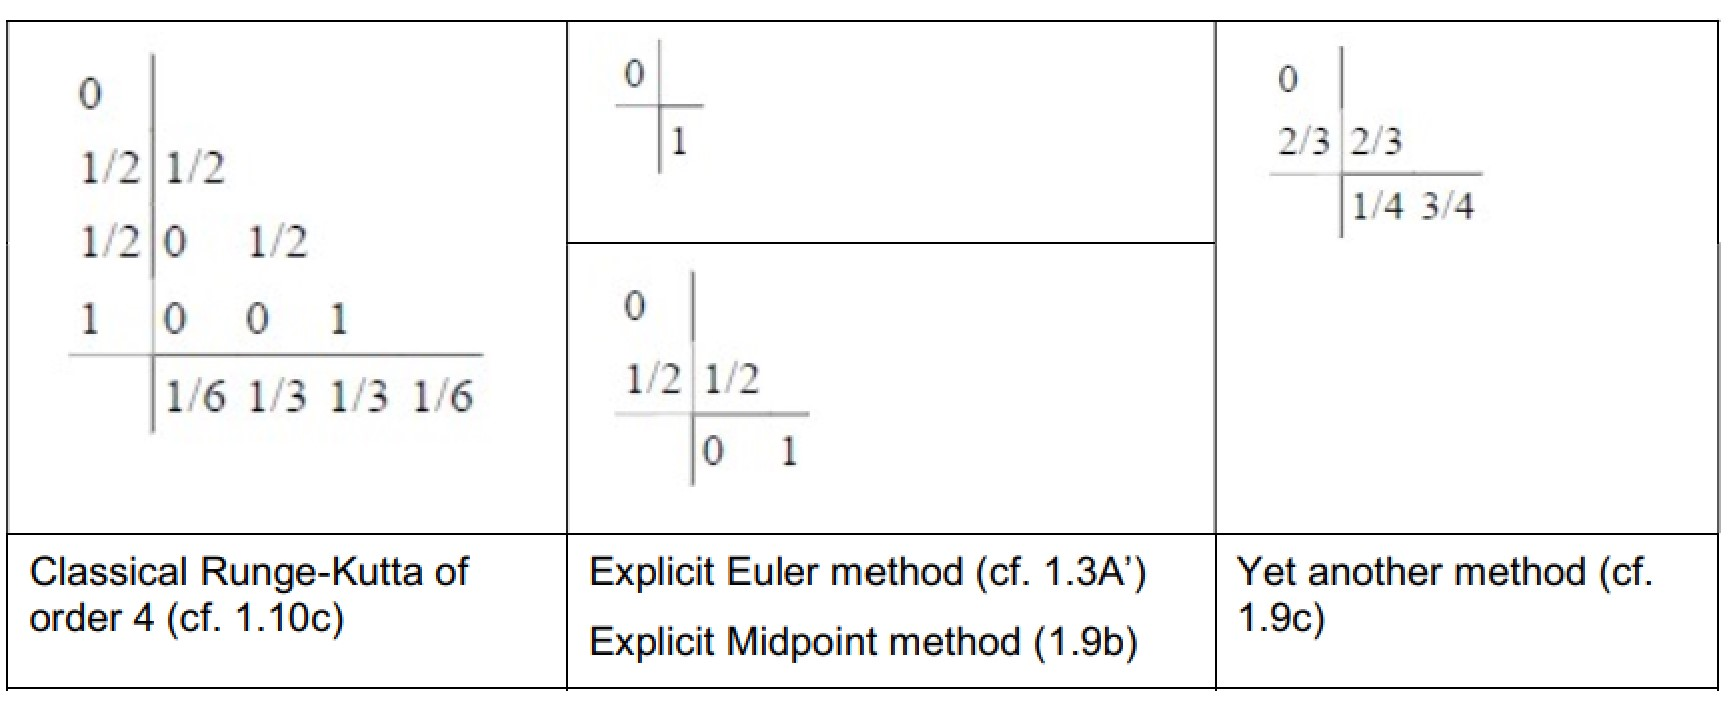
\includegraphics{images/butcher_tableaus.jpg}}
  \caption{Butcher Tableaus}
  \label{table:butcher_tableaus}
\end{table}\newline
\href{https://en.wikipedia.org/wiki/List_of_Runge%E2%80%93Kutta_methods}{The simplest adaptive Runge–Kutta method involves combining Heun's method, which is order 2, with the Euler method, which is order 1} (also called Heun-Euler 2(1)). Its extended Butcher Tableau can be seen in \autoref{eq:heun_euler_2_1}. 
\begin{equation}\label{eq:heun_euler_2_1}
\begin{array}{c|cc}
0 & & \\
1 & 1 & \\
\hline & 1 / 2 & 1 / 2 \\
& 1 & 0
\end{array}
\end{equation}

\subsection{Step-size adaption}
\subsubsection{Idea}
The Idea is to automatically adapt the step-size $h$. Due to that one needs a new way to define the approximation of the error, which can be done with an Accuracy Goal $(ac)$, which defines how many decimal places (Nachkommastellen) are correct and a precision Goal $(pg)$, which represents the significant digits of the result. The two parameters are considered in the tolerance parameter, $\varepsilon$ which can be found in \autoref{eq:tolerance_parameter}.
\begin{equation}\label{eq:tolerance_parameter}
    \varepsilon=\varepsilon_{a}+|y| \varepsilon_{r}=10^{-a g}+|y| 10^{-p g} \geq|e|
\end{equation}
Furthermore, one needs a second approximation for the error calculation, with the order $\hat{p}$. The first order approximation $p$ is needed to calculate the step size. Mostly $\hat{p}=p-1$. Due to that the butcher tableau is extended by a row ($b$ values) as it can be seen in \autoref{table:butcher_2}.
\begin{table}[ht]
\centering
\begin{tabular}{|c|ccccc|}
\hline 0 & 0 & 0 & $\cdots$ & 0 & 0 \\
$c_{2}$ & $a_{2,1}$ & 0 & $\cdots$ & 0 & 0 \\
$\vdots$ & $\vdots$ & $\vdots$ & $\ddots$ & 0 & $\vdots$ \\
$c_{s-1}$ & $a_{s-1,1}$ & $a_{s-1,2}$ & $\cdots$ & 0 & 0 \\
$c_{s}$ & $a_{s, 1}$ & $a_{s, 2}$ & $\cdots$ & $a_{s, s-1}$ & 0 \\
\hline & $b_{1}$ & $b_{2}$ & $\cdots$ & $b_{s-1}$ & $b_{s}$ \\
& $\hat{b}_{1}$ & $\hat{b}_{2}$ & $\cdots$ & $\hat{b}_{s-1}$ & $\hat{b}_{s}$ \\
\hline
\end{tabular}
\caption{Butcher Table}
\label{table:butcher_2}
\end{table}
The local error can be calculated according to \autoref{eq:adaptive_local_error}.
\begin{equation}\label{eq:adaptive_local_error}
    e_{n}=y(x+h)-\hat{y}(x+h)=h_{n} \sum_{j=1}^{s}\left(b_{j}-\hat{b}_{j}\right) k_{j} \Rightarrow\left\|e_{n}\right\|=\left\|h_{n} \sum_{j=1}^{s}\left(b_{j}-\hat{b}_{j}\right) k_{j}\right\|
\end{equation}
Below one can find again a short description of the variables:
\begin{itemize}
    \item $\varepsilon_{a}=dy$: absolute error $\varepsilon_{a}=10^{-ag}$ \newline
    Ex. $ag=4 \Rightarrow 0.\textcolor{red}{0012}89$
    \item $\varepsilon_{r}=\frac{dy}{y\ne 0}$: relative error $\varepsilon_{r}=10^{-pg}$\newline
    Ex. $pg=4 \Rightarrow 0.00\underbrace{\textcolor{red}{1289}}_{\text{signific. digit}}$
\end{itemize}


To know if the step size is good or not one calculates $\frac{\left\|e_{n}\right\|}{\varepsilon}$. When the current step $\frac{\left\|e_{n}\right\|}{\varepsilon}>1$, then the estimation of $h_{n}$ was too optimistic and the step must be repeated with a smaller step size. One also says the current step is \textbf{Rejected}. Otherwise when $\frac{\left\|e_{n}\right\|}{\varepsilon}\leq 1$ the step size is ok and one can \textbf{proceed}.
Updating the step size is done according to \autoref{eq:step_size}.
\begin{equation}\label{eq:step_size}
    h_{n+1}=h_{n}\left(\frac{\varepsilon}{\left\|e_{n}\right\|}\right)^{\frac{1}{\bar{p}}}=h_{n}\left(\frac{\left\|e_{n}\right\|}{\varepsilon}\right)^{-\frac{1}{\bar{p}}}
\end{equation}
$\varepsilon=\varepsilon_{a}+\varepsilon_{r}\left|y_{n}\right| \quad$ with $\quad \tilde{p}=\min (p, \hat{p})+1$ (order of the primary method)


\subsubsection{Stability of explicit methods}
The global relative error must not diverge, which means it must be limited. Since it is difficult to make a statement about the analysed ODE one uses benchmark equations. One of the most commonly used ones is the Dahlquist model, which can be seen in \autoref{eq:dahlquist}
\begin{equation}\label{eq:dahlquist}
    y^{\prime}=A y \quad y(0)=1 \quad \text { mit } A=\Re\{A\}+j \Im\{A\} \in \mathbb{C}
\end{equation}
The solution of this equation is $y=e^{\Re\{A\} x}\left(\cos (\Im\{A\} x+j \sin (\Im\{A\} x))\right.$, which is an oscillation with a exponential amplitude $e^{\Re\{A\} x}$ and  frequency $\Im\{A\}$. The 
\paragraph{Example Euler}
$$
Y^{\prime}=-\lambda Y ; Y(0)=1 ; x \geq 0 ; \lambda>0
$$
The exact solution is: $\quad Y(x)=e^{-\lambda x}$
Consider Euler's method: Solation will go to zero iff
$$
\begin{aligned}
y_{n+1} & =y_n+h f\left(x_n, y_n\right) & & |1-h \lambda|<1 \Rightarrow \frac{2}{\lambda}>h>0 \\
& =y_n-h \lambda y_n & & \text { Euler's method is stable for } \\
& =(1-h \lambda) y_n & & \text { this ODE if } \quad 0<h<\frac{2}{\lambda}
\end{aligned}
$$
\paragraph{Stability for heun-method (rk-2)}\mbox{}\newline
From \autoref{eq:general_runge_kutta} one knows that $y_{k+1}=y_k+h\cdot (\frac{1}{2}\cdot k_1+\frac{1}{2}\cdot k_2)$
\begin{equation}
\begin{array}{lc}
k_{1}=A y_{k} & y_{0}=y\left(x_{0}\right)=y(0)=1 \\
k_{2}=A\left(y_{k}+1 h k_{1}\right)=A\left(y_{k}+A h y_{k}\right) \quad \Longrightarrow \quad &y_{k+1}=y_{k} \underbrace{\left(1+h A+(h A)^{2} \frac{1}{2}\right)}_{F(h A)=F(z), \quad z=h A \in \mathbb{C}}
\end{array}
\end{equation}
From that one can somehow derive three cases which are listed below


\paragraph{3 Cases}
\begin{itemize}
    \item $\Re\{A\}<0$: The Amplitude of the ODE gets smaller exponentially. The stability conditions says that the approximated values $y_{k}(k=0,1, \ldots)$ must be exponentially damped too. Therefore and from $y_{k+1} \propto|F(z)|$ the following must hold $|F(z)|<1$.
    \item $\Re\{A\}=0$ : The Amplitude of the ODE is constant. The stability conditions says that the approximated values $y_{k}(k=0,1, \ldots)$ are constant too. Therefore and from $y_{k+1} \propto|F(z)|$ the following must hold $|F(z)|=1$.
    \item $\Re\{A\}>0$ : The Amplitude of the ODE gets larger exponentially. The stability conditions says that the approximated values $y_{k}(k=0,1, \ldots)$ must be exponentially growing too. Therefore and from $y_{k+1} \propto|F(z)|$ the following must hold $|F(z)|>1$.
\end{itemize}
The stability condition for case one can know be calculated as the following $(\Re\{A\}<0)$ and $1>|F(z)|=\left|1+h A+\frac{1}{2}(h A)^{2}\right| \Rightarrow-2<h \Re\{A\}<0$.  since $x_{1,2}=\frac{-b \pm \sqrt{(b^2-4\cdot a \cdot c)}}{2 \cdot a}=\frac{-1 \pm \sqrt{((1)^2-4\cdot 0 \cdot \frac{1}{2})}}{2 \cdot \frac{1}{2}}=-1 \pm 1$ and therefore the values must be between 0 and -2. The \textbf{stability polynomial} in this exercise was $F(z)=1+z+\frac{z^2}{2} \quad(z=h A)$.
\paragraph{Recursive Formulas}\mbox{}\newline
For the stability polynomials in the form: $F(z)=1+b_{1} k_{1}(z)+\ldots+b_{s} k_{s}(z)$ recursive equations exist as can be seen in \autoref{eq:recursive_formula}.
\begin{equation}\label{eq:recursive_formula}
 k_{1}(z)=z, \quad k_{j+1}(z)=z\left(1+a_{j+1,1} k_{1}(z)+a_{j+1,2} k_{2}(z)+\ldots+a_{j+1, j} k_{j}(z)\right)
\end{equation}
\subsubsection{Exercise adaptive step size}
Solve the initial value problem $\varphi^{\prime}=c(1-\varepsilon \cos \varphi)^2 \quad \varphi(0)=0$ with $c=1$ and $\epsilon=0.25$ numerically by applying the Heun-Euler 2(1) embedded adaptive method with classical step-size control until 3 proceeding steps are executed. The initial step-size equals $0.001$, the accuracy goal (ag) 4 and the precision goal is 4 , either.\newline
Create a table listing values for $\left(x, y, h, e_k,\left(\frac{\left\|e_k\right\|}{\varepsilon}\right)^{-\frac{1}{\widetilde{p}}}, h_{\text {new }}\right.$, state $)$ containing at least three preceding steps.\newline 
According to the exercise, we know the following:
\begin{enumerate}
    \item The position at the beginning: $x=0$, $y=0$
    \item The step size: $h=0.001$
    \item The local error can be calculated according to \autoref{eq:adaptive_local_error}. Which says that $e_{k}=h_{n} \sum_{j=1}^{s}\left(b_{j}-\hat{b}_{j}\right) k_{j}$. From \autoref{eq:heun_euler_2_1} one knows $b_1=\frac{1}{2}$, $\hat{b}_1=1$, $b_2=\frac{1}{2}$ and $\hat{b}_2=0$. Furthermore, one knows from \autoref{eq:general_runge_kutta} and \autoref{eq:heun_euler_2_1} that $k_1=f\left(x_n+\underbrace{0}_{c_1}\cdot h_n, y_n+h_n\cdot \underbrace{0}_{a_{1,j}} \right)=1\cdot \left(1-\frac{1}{4} \cos{0}\right)^2=\textcolor{blue}{\frac{9}{16}}$ and 
    $k_2=f\left(x_n\textcolor{gray}{+\underbrace{\xout{1}}_{c_2}\cdot \xout{h_n}}, y_n+h_n\cdot \underbrace{1}_{a_{2,1}}\cdot k_1\right)=1 \cdot \left(1-(\frac{1}{4}\cdot \cos{(0.001\cdot 1 \cdot \textcolor{blue}{\frac{9}{16}})}\right)^2=\textcolor{orange}{0.5625}$. Therefore $e_k=h_n\cdot (b_1-\hat{b}_1)\cdot k_1+(b_2-\hat{b}_2)\cdot k_2=\underbrace{0.001}_{h_n}\cdot (\underbrace{-\frac{1}{2}}_{b_1-\hat{b}_1}\cdot\textcolor{blue}{\frac{9}{16}} + \underbrace{\frac{1}{2}}_{(b_2-\hat{b}_2)} \cdot \textcolor{orange}{0.5625} )= \textcolor{brown}{2.966\cdot 10^{-11}}$
    \item Since $p=2$ (order) and $\varepsilon$ can be calculated according to \autoref{eq:tolerance_parameter} which says: $\varepsilon=\varepsilon_{a}+|y| \varepsilon_{r}=10^{-a g}+|y| 10^{-p g} = 10^{-4}+0 \cdot  10^{-4}=10^{-4}$. Therefore $\left(\frac{\left\|e_k\right\|}{\varepsilon}\right)^{-\frac{1}{\widetilde{p}}}=\left(\frac{\textcolor{brown}{2.966\cdot 10^{-11}}}{10^{-4}}\right)^{-\frac{1}{2}}=1.836\cdot 10^3$
    \item With \autoref{eq:step_size} one can the finally calculate the new step size which is: $h_{n+1}=h_{n}\left(\frac{\left\|e_{n}\right\|}{\varepsilon}\right)^{-\frac{1}{\bar{p}}}=0.001\cdot \left(\frac{\textcolor{brown}{2.966\cdot 10^{-11}}}{10^{-4}}\right)^{-\frac{1}{2}}=1.836$
    \item the new y value can be calculated according to \autoref{eq:general_runge_kutta} which means for the current scheme $0.001\cdot (\frac{1}{2}\cdot k_1+\frac{1}{2}\cdot k_2)=0.001\cdot (\frac{1}{2}\cdot \textcolor{blue}{\frac{9}{16}}+\frac{1}{2}\cdot \textcolor{orange}{0.5625})=0.0005625$
\end{enumerate}

\begin{table}[ht]
    \centering
    \begin{tabular}{|c|c|c|c|c|c|c|}
    \hline x & y &  $h_n$ & $e_k$ & $\left(\frac{\left\|e_k\right\|}{\varepsilon}\right)^{-\frac{1}{\widetilde{p}}}$ & $h_{n+1}$&state\\
    \hline
    0& 0& 0.001 &$\textcolor{brown}{2.966\cdot 10^{-11}}$&$1.836\cdot 10^3$&1.836&Proceed\\
    \hline
    0.001& 0.0005625&1.836&0.18169&0.02347&0.043&Reject\\
    \hline
    \end{tabular}
    \caption{Exercise}
    \label{tab:example_tab}
\end{table}

\subsubsection{Exercise Stability polynomial}
Using Theorem $1.3$ in the script (p. 29) gain the A-stability polynomial $F_1(z)=1+z+\frac{z^2}{2}+\frac{z^3}{6}$ for the embedded adaptive method SS3(2) with Butcher tableau.
$$
\begin{array}{c|cccc}
0\\
\frac{1}{2} & \textcolor{orange}{\frac{1}{2}} & & \\
1 & \textcolor{brown}{-1} & \textcolor{blue}{2} &  \\
1 &  \frac{1}{6} & \frac{2}{3} & \frac{1}{6} \\
\hline
&\textcolor{pink}{\frac{1}{6}} & \textcolor{purple}{\frac{2}{3}} & \frac{1}{6}&0 \\
&\frac{1}{72}(\sqrt{82}-10) & \frac{1}{36}(10-\sqrt{82}) & \frac{1}{144}(28-\sqrt{82}) & \frac{1}{48}(\sqrt{82}-16)
\end{array}
$$
From \autoref{eq:recursive_formula} one knows that a stability polynomial is of the form $F(z)=1+b_1 k_1(z)+b_2 k_2(z)+b_3 k_3(z)+0 k_4(z)$, whereas:
$$
\begin{aligned}
& k_1(z)=z \\
& k_2(z)=z\left(1+\textcolor{orange}{\frac{1}{2}} k_1(z)\right)=z\left(1+\frac{1}{2} z\right) \\
& k_3(z)=z\left(1+\textcolor{brown}{-1} k_1(z)+\textcolor{blue}{2} k_2(z)\right)=z\left(1-z+2 z\left(1+\frac{1}{2} z\right)\right)=z+z^2+z^3
\end{aligned}
$$
$$
\text { Therefore } F(z)=1+\textcolor{pink}{\frac{1}{6}} k_1(z)+\textcolor{purple}{\frac{2}{3}} k_2(z)+\frac{1}{6} k_3(z)=1+z+\frac{1}{2} z^2+\frac{1}{6} z^3
$$
\subsubsection{Stiffness}\label{subsubsec:stiffnes}

The stiffnes is dependent on:
\begin{itemize}
    \item ODE
    \item step size h
    \item Method (for example RK-4)
\end{itemize}
\paragraph{Stiffness Detection}\mbox{}\newline
Heun euler does not work when we have stiffness situations.
Condition: $c_{s-1}=c_{s}=1$. Through testing of $\left|h \frac{\partial f(x, y)}{\partial y}\right|$ to the absolute borders of the stability region the stiffness can be detected. Stiffness is present when $|h \tilde{\lambda}|$ is outside or at the border of the stability condition.

\paragraph{Example for explicit runge-kutta}\mbox{}\newline
$$
k_{s-1}=f(x+c_{s-1} h, \underbrace{y+h \sum_{j=1}^{s} a_{s-1, j} k_{j}}_{g_{s-1}}) \quad k_{s}=f(x+c_{s} h, \underbrace{\left.y+h \sum_{j=1}^{s} a_{s, j} k_{j}\right)}_{g_{s}} \quad \Rightarrow \quad \tilde{\lambda}=\frac{\left\|k_{s}-k_{s-1}\right\|}{\left\|g_{s}-g_{s-1}\right\|}
$$
$\tilde{\lambda}$ is an estimation for $f_{y}=\frac{\partial}{\partial y} f(x, y)$ for example $y^{\prime}=x^{4}-25 y^{4}=f(x, y)$ and takes the role of $\Re\{A\}$ for the stability analysis.




\subsubsection{Exercise stiffness detection test}
Given the differential equation $y^{\prime}=\underbrace{-\sqrt{x^2+y^2}}_{f(x, y)} \quad y(0)=4 \quad$ carry out a stiffness detection test using the A-stability region and the partial derivative $f_y$ at the initial values and step size $h=1$. The method is defined by the Butcher tableau below.
$$
\begin{array}{l|ll}
0 & & \\
1 / 2 & \textcolor{orange}{1 / 2} & \\
b & \textcolor{pink}{0} & \textcolor{purple}{1} \\
\hat{b} & 1 & 0 \\
\hline
\end{array}
$$
The exercise can be solved in two steps:
\begin{enumerate}
    \item Get stability region (\autoref{eq:recursive_formula}):\newline
    From \autoref{eq:recursive_formula} one knows that a stability polynomial is of the form $F(z)=1+b_1 k_1(z)+b_2 k_2(z)+b_3 k_3(z)+0 k_4(z)$, whereas:
    $$
    \begin{aligned}
    & k_1(z)=z \\
    & k_2(z)=z\left(1+\textcolor{orange}{\frac{1}{2}} k_1(z)\right)=z\left(1+\frac{1}{2} z\right) \\
    \end{aligned}
    $$
    $$
    \text { Therefore } F(z)=1+\textcolor{pink}{0} k_1(z)+\textcolor{purple}{1} k_2(z)=1+z+\frac{1}{2} z^2 \text{ where } (z=h\cdot A)
    $$
    To calculate the stability region one hast to set the stability polynomial to zero and therefore one gets: $x_{1,2}=\frac{-b \pm \sqrt{(b^2-4\cdot a \cdot c)}}{2 \cdot a}=\frac{-1 \pm \sqrt{((1)^2-4\cdot 0 \cdot \frac{1}{2})}}{2 \cdot \frac{1}{2}}=-1 \pm 1$ and therefore the boundary is -2 and 0.
    \item Check stiffness (see \autoref{subsubsec:stiffnes})\newline
     By calculating the partial derivative of $-\sqrt{x^2+y^2}$ after y one obtains the following $-1\cdot \frac{1}{2}\cdot \frac{1}{\sqrt{x^2+y^2}} \cdot 2 \cdot y$ inserting $x=0$ and $y=4$ results in  $-1\Rightarrow A=-1$ and $h\cdot A =-1$ which is inside the A-stability constraint $-2<Ah<0$ and therefore no stiffness is detected.
\end{enumerate}

\subsubsection{Van der Pol second-order differential equation}
Solve the van-der-Pol ODE-system $\left(\begin{array}{l}z^{\prime}=v \\ v^{\prime}=\mu\left(1-z^2\right) v-z\end{array}\right) \quad z(0)=1, v(0)=-1, \quad \mu=0.2$ numerically by applying the Heun-Euler 2(1) embedded adaptive method with classical step-size control until 3 proceeding steps are executed. The initial step-size equals $0.001$, the accuracy goal (ag) 1 and the precision goal is 2.
Create a table listing values for $\left(t,\{z, v\}, h, e_k,\left\|\frac{\vec{e}_n}{\varepsilon_a+\varepsilon_r \vec{y}_n}\right\|^{-1 / \tilde{p}}, h_{\text {new, }}\right.$ state) containing at least three proceeding steps.

According to the exercise, we know the following:
\begin{enumerate}
    \item The position at the beginning: $x=0$, $z=0, v=-1$
    \item The step size: $h=0.001$
    \item The local error can be calculated according to \autoref{eq:adaptive_local_error}. Which says that $e_{k}=h_{n} \sum_{j=1}^{s}\left(b_{j}-\hat{b}_{j}\right) k_{j}$. From \autoref{eq:heun_euler_2_1} one knows $b_1=\frac{1}{2}$, $\hat{b}_1=1$, $b_2=\frac{1}{2}$ and $\hat{b}_2=0$. Furthermore, one knows from \autoref{eq:general_runge_kutta} and \autoref{eq:heun_euler_2_1} that $k_1=f\left(x_n+\underbrace{0}_{c_1}\cdot h_n, y_n+h_n\cdot \underbrace{0}_{a_{1,j}} \right)=
    \left[\begin{array}{cc}
    v \\ 
    v^{\prime}=\mu\left(1-z^2\right) v-z
    \end{array}\right]=
    \left[\begin{array}{cc}
    -1\\
    0.2(1-1^2)\cdot (-1)-1
    \end{array}\right]=
    \textcolor{blue}{\left[\begin{array}{cc}
    -1\\
    -1
    \end{array}\right]}$ and 
    $$\begin{aligned}k_2&=f\left(x_n+\underbrace{0}_{c_2}\cdot h_n, y_n+h_n\cdot \underbrace{1}_{a_{2,1}}\cdot k_1\right)\\&=
    \left[\begin{array}{cc}
    -1+0.001\cdot 1\cdot \textcolor{blue}{(-1)} \\ 
    0.2(1-(1+0.001\cdot 1 \cdot \textcolor{blue}{(-1)})^2)\cdot (-1+ 0.001\cdot 1 \cdot \textcolor{blue}{(-1)})-(1+0.001\cdot 1 \cdot \textcolor{blue}{(-1)})
    \end{array}\right]\\&=
    \textcolor{orange}{\left[\begin{array}{cc}
    -1.001\\ 
    -0.9994001998
    \end{array}\right]}\end{aligned}$$
    
    Therefore $e_k=0.001\cdot (-\frac{1}{2}\cdot\textcolor{blue}{\left[\begin{array}{cc}
    -1\\
    -1
    \end{array}\right]} + \frac{1}{2} \cdot \textcolor{orange}{\left[\begin{array}{cc}
    -1.001\\ 
    -0.9994001998
    \end{array}\right]} )= \textcolor{brown}{\left[\begin{array}{cc}
    -5\cdot 10^{-1}\\ 
    2.999001\cdot 10^{-1}
    \end{array}\right]}$
    
    \item Sine $p=2$ (order) and $\varepsilon$ can be calculated according to \autoref{eq:tolerance_parameter} which says: $\varepsilon=\varepsilon_{a}+|y| \varepsilon_{r}=10^{-a g}+|y| 10^{-p g} = 10^{-1}+\left[\begin{array}{cc}
    1\\
    -1
    \end{array}\right] \cdot  10^{-2}=\left[\begin{array}{cc}
    0.11\\
    0.09
    \end{array}\right]$. Therefore $\left(\frac{\left\|e_k\right\|}{\varepsilon}\right)^{-\frac{1}{\widetilde{p}}}=\left(\max \left(\operatorname{abs}\left(\textcolor{brown}{\left[\begin{array}{cc}
    -5\cdot 10^{-1}\\ 
    2.999001\cdot 10^{-1}
    \end{array}\right]} ./\left(\left(\left[\begin{array}{l}
    0.11 \\
    0.09
    \end{array}\right]\right)\right)\right)\right)^{\frac{-1}{2}}\right.=469.04157598235$
    
    \item With \autoref{eq:step_size} one can the finally calculate the new step size which is: $h_{n+1}=h_{n}\left(\frac{\left\|e_{n}\right\|}{\varepsilon}\right)^{-\frac{1}{\bar{p}}}=0.001\cdot 469.04157598235=\textcolor{violet}{0.46904157598235}$
    
    \item the new y value can be calculated according to \autoref{eq:general_runge_kutta} which means for the current scheme $0.001\cdot (\frac{1}{2}\cdot k_1+\frac{1}{2}\cdot k_2)=0.001\cdot (\frac{1}{2}\cdot \textcolor{blue}{\left[\begin{array}{cc}
    -1\\
    -1
    \end{array}\right]}+\frac{1}{2}\cdot \textcolor{orange}{\left[\begin{array}{cc}
    -1.001\\ 
    00.9994001998
    \end{array}\right]})=\textcolor{pink}{\left[\begin{array}{cc}
    0.9989995\\ 
    -1.0009997000999
    \end{array}\right]}$
\end{enumerate}

\begin{table}[ht]
    \centering
    \begin{tabular}{|c|c|c|c|c|c|c|}
    \hline x & y &  $h_n$ & $e_k$ & $\left(\frac{\left\|e_k\right\|}{\varepsilon}\right)^{-\frac{1}{\widetilde{p}}}$ & $h_{n+1}$&state\\
    \hline
    0& $\left[\begin{array}{cc}
    1\\
    -1
    \end{array}\right]$& 0.001 &$\textcolor{brown}{\left[\begin{array}{cc}
    -5\cdot 10^{-1}\\ 
    2.999001\cdot 10^{-1}
    \end{array}\right]}$&$469.04157598235$&$\textcolor{violet}{0.46904}$&Proceed\\
    \hline
    0.001& $\textcolor{pink}{\left[\begin{array}{cc}
    0.9989995\\ 
    -1.0009997000999
    \end{array}\right]}$&0.46904157598235&&&&Reject\\
    \hline
    \end{tabular}
    \caption{Exercise}
    \label{tab:example_tab}
\end{table}

\begin{equation}
z^{\prime \prime}(t)=\underbrace{\mu\left(1-z^2\right)}_{\text {non-linear damping }} z^{\prime}-z
\end{equation}

\begin{equation}
\begin{aligned}
& z^{\prime}=z_1 \\
& z_1^{\prime}=z_2 \\
& z_2{ }^{\prime}=z_3 \\
& \quad \vdots \\
& z_{n-1}{ }^{\prime}=f\left(x, z, z_1, z_2, \cdots, z_{n-1}\right)
\end{aligned}
\end{equation}

\begin{equation}
\begin{aligned}
z^{\prime} & =v \\
z_1^{\prime} & =\mu\left(1-z^2\right) z_1-z
\end{aligned}
\end{equation}



\begin{equation}
\begin{aligned}
\vec{y}^{\prime \prime}(x)&=\frac{\overrightarrow{d f}}{d x}=J_{\vec{f}}(x, \vec{y}) \cdot\left(1, \vec{y}^{\prime}(x)\right)^{t r}=(\frac{\partial \vec{f}}{\partial x}, \underbrace{\frac{\partial \vec{f}}{\partial y_1}, \frac{\partial \vec{f}}{\partial y_2}, \cdots, \frac{\partial \vec{f}}{\partial y_m}}_{=: \frac{\partial \vec{f}}{\partial \vec{y}}=J_{\bar{f}}(\vec{y})})\cdot (1, \underbrace{y_1^{\prime}(x), y_2^{\prime}(x), \cdots, y_m^{\prime}(x)}_{=: y^{\prime}(x)})^{t r}\\&=
 \frac{\partial \vec{f}}{\partial x}+\frac{\partial \vec{f}}{\partial \vec{y}} \cdot \vec{y}^{\prime}(x):=\vec{f}_x+\vec{f}_{\dot{y}} \cdot \vec{f}:=\vec{F}_1 \\
\end{aligned}
\end{equation}

 \begin{equation}
\vec{f}(t, z, v)=\left(\begin{array}{lc}
f_1(t, z, v)= & v \\
f_2(t, z, v)= & \mu\left(1-z^2\right) v-z
\end{array}\right)
\end{equation}


\section{Fromulas}
\subsection{Differentation Formulas}
\begin{multicols}{2}
[]
 \begin{enumerate}
     \item $\frac{\mathrm{d}(u \pm v)}{\mathrm{d} x}=\frac{\mathrm{d} u}{\mathrm{~d} x} \pm \frac{\mathrm{d} v}{\mathrm{~d} x}$
    \item $\frac{\mathrm{d}(k \cdot u)}{\mathrm{d} x}=k \cdot \frac{\mathrm{d} u}{\mathrm{~d} x} \quad(k$ konstant $)$
    \item $\frac{\mathrm{d}(u \cdot v)}{\mathrm{d} x}=\frac{\mathrm{d} u}{\mathrm{~d} x} \cdot v+u \cdot \frac{\mathrm{d} v}{\mathrm{~d} x}$
    \item $\frac{\mathrm{d}(u / v)}{\mathrm{d} x}=\frac{\frac{\mathrm{d} u}{\mathrm{~d} x} v-u \mathrm{~d} v}{v^{2}}$
    \item $\frac{\mathrm{d} z}{\mathrm{~d} x}=\frac{\mathrm{d} z}{\mathrm{~d} y} \cdot \frac{\mathrm{d} y}{\mathrm{~d} x} \quad$ falls $z=f(y)$ und $y=g(x)$
    \item $\frac{\mathrm{d}}{\mathrm{d} x}\left(x^{n}\right)=n x^{n-1}$
    \item $\frac{\mathrm{d}}{\mathrm{d} x}\left(\mathrm{e}^{x}\right)=\mathrm{e}^{x}$
    \item $\frac{\mathrm{d}}{\mathrm{d} x}\left(a^{x}\right)=a^{x} \ln a \quad(a>0)$
    \item $\frac{\mathrm{d}}{\mathrm{d} x}(\ln x)=\frac{1}{x}$
    \item $\frac{\mathrm{d}}{\mathrm{d} x}(\sin x)=\cos x$
    \item $\frac{\mathrm{d}}{\mathrm{d} x}(\cos x)=-\sin x$
    \item $\frac{\mathrm{d}}{\mathrm{d} x}(\tan x)=\frac{1}{\cos ^{2} x}$
    \item $\frac{\mathrm{d}}{\mathrm{d} x}(\arcsin x)=\frac{1}{\sqrt{1-x^{2}}}$
    \item $\frac{\mathrm{d}}{\mathrm{d} x}(\arctan x)=\frac{1}{1+x^{2}}$
 \end{enumerate}
\end{multicols}
\subsection{Integration Formulas}
\begin{multicols}{2}
[]
 \begin{enumerate}
    \item $\int_{a}^{b}(u \pm v) \mathrm{d} x=\int_{a}^{b} u \mathrm{~d} x \pm \int_{a}^{b} v \mathrm{~d} x$
    \item $\int_{a}^{b} k \cdot u \mathrm{~d} x=k \int_{a}^{b} u \mathrm{~d} x \quad(k$ konstant $)$
    \item $\int_{x=a}^{b} f(g(x)) g^{\prime}(x) \mathrm{d} x=\int_{w=g(a)}^{g(b)} f(w) \mathrm{d} w$
    \item $\int_{a}^{b} u \cdot \frac{\mathrm{d} v}{\mathrm{~d} x} \mathrm{~d} x=\left.(u \cdot v)\right|_{a} ^{b}-\int_{a}^{b} \frac{\mathrm{d} u}{\mathrm{~d} x} \cdot v \mathrm{~d} x$
 \end{enumerate}
\end{multicols}

\subsection{Table of Indefinite Integrals}
\begin{multicols}{2}
[\subsubsection{Basic Functions}]
 \begin{enumerate}
\item $\int x^{n} \mathrm{~d} x=\frac{1}{n+1} x^{n+1}+C, n \neq-1$
\item $\int \frac{1}{x} \mathrm{~d} x=\ln |x|+C$
\item $\int a^{x} \mathrm{~d} x=\frac{1}{\ln a} a^{x}+C, a>0$
\item $\int \ln x \mathrm{~d} x=x \ln x-x+C$
\item $\int \sin x \mathrm{~d} x=-\cos x+C$
\item $\int \cos x \mathrm{~d} x=\sin x+C$
\item $\int \tan x \mathrm{~d} x=-\ln |\cos x|+C$
 \end{enumerate}
\end{multicols}


\subsubsection{Products of $e^x$ and cox x and sin x}
 \begin{enumerate}
    \setcounter{enumi}{7}
    \item $\begin{aligned}
        \int \mathrm{e}^{a x} \sin (b x) \mathrm{d} x=\frac{1}{a^{2}+b^{2}} \mathrm{e}^{a x}(a \sin (b x)-b \cos (b x))+C\end{aligned}$ 
    \item $\begin{aligned}
        \int \mathrm{e}^{a x} \cos (b x) \mathrm{d} x=\frac{1}{a^{2}+b^{2}} \mathrm{e}^{a x}(a \cos (b x)+b \sin (b x))+C\end{aligned}$ 
    \item $\begin{aligned} 
        \int \sin (a x) \sin (b x) \mathrm{d} x=\frac{1}{b^{2}-a^{2}}(a \cos (a x) \sin (b x)-b \sin (a x) \cos (b x))+C, a \neq b\end{aligned}$ 
    \item $\begin{aligned} 
        \int \cos (a x) \cos (b x) \mathrm{d} x=\frac{1}{b^{2}-a^{2}}(b \cos (a x) \sin (b x)-a \sin (a x) \cos (b x))+C, a \neq b\end{aligned}$
    \item $\begin{aligned} 
        \int \sin (a x) \cos (b x) \mathrm{d} x=\frac{1}{b^{2}-a^{2}}(b \sin (a x) \sin (b x)+a \cos (a x) \cos (b x))+C, a \neq b\end{aligned}$
 \end{enumerate}

\subsubsection{Product of Polynomial $p(x)$ with $\ln x, \mathrm{e}^{x}, \cos x, \sin x$}
 \begin{enumerate}
    \setcounter{enumi}{12}
    \item $\begin{aligned} 
        \int x^{n} \ln x \mathrm{~d} x=\frac{1}{n+1} x^{n+1} \ln x-\frac{1}{(n+1)^{2}} x^{n+1}+C, n \neq-1\end{aligned}$
    \item $\begin{aligned} 
        \int p(x) \mathrm{e}^{a x} \mathrm{~d} x=\frac{1}{a} p(x) \mathrm{e}^{a x}-\frac{1}{a} \int p^{\prime}(x) \mathrm{e}^{a x} \mathrm{~d} x=\frac{1}{a} p(x) \mathrm{e}^{a x}-\frac{1}{a^{2}} p^{\prime}(x) \mathrm{e}^{a x}+\frac{1}{a^{3}} p^{\prime \prime}(x) \mathrm{e}^{a x}-\ldots\end{aligned}$\newline
        (Sign alternate: $+-+-+-\ldots$ )
    \item $\begin{aligned}
        \int p(x) \sin (a x) \mathrm{d} x&=-\frac{1}{a} p(x) \cos (a x)+\frac{1}{a} \int p^{\prime}(x) \cos (a x) \mathrm{d} x\\ &=-\frac{1}{a} p(x) \cos (a x)+\frac{1}{a^{2}} p^{\prime}(x) \sin (a x)+\frac{1}{a^{3}} p^{\prime \prime}(x) \cos (a x)-\ldots 
        \end{aligned}$\newline 
        (Sign alternate in pairs after first term: $-++-++\ldots$ )
    \item $\begin{aligned}
        \int p(x) \cos (a x) \mathrm{d} x&=\frac{1}{a} p(x) \sin (a x)-\frac{1}{a} \int p^{\prime}(x) \sin (a x) \mathrm{d} x\\
        &=\frac{1}{a} p(x) \sin (a x)+\frac{1}{a^{2}} p^{\prime}(x) \cos (a x)-\frac{1}{a^{3}} p^{\prime \prime}(x) \sin (a x)-\ldots
    \end{aligned}$\newline
    (Signs alternate in pairs: $++--++-\ldots$ )
 \end{enumerate}

\subsection{Taylor Polynomial/Series}
Development of $f$ around $a$
$$
\begin{aligned}
f(x) & \approx f(a)+f^{\prime}(a)(x-a)+\frac{f^{\prime \prime}(a)}{2 !}(x-a)^{2}+\frac{f^{\prime \prime \prime}(a)}{3 !}(x-a)^{3}+\ldots \\
f(a+h) & \approx f(a)+f^{\prime}(a) h+\frac{f^{\prime \prime}(a)}{2 !} h^{2}+\frac{f^{\prime \prime \prime}(a)}{3 !} h^{3}+\ldots
\end{aligned}
$$
in which $k !=1 \cdot 2 \cdot 3 \cdot \ldots \cdot k$.
\subsubsection{Important Taylor Series}
$$
\begin{aligned}
\mathrm{e}^{x} & =1+x+\frac{1}{2 !} x^{2}+\frac{1}{3 !} x^{3}+\ldots \\
\cos x & =1-\frac{1}{2 !} x^{2}+\frac{1}{4 !} x^{4}-\frac{1}{6 !} x^{6}+\ldots \\
\sin x & =x-\frac{1}{3 !} x^{3}+\frac{1}{5 !} x^{5}-\frac{1}{7 !} x^{7}+\ldots \\
\frac{1}{1-x} & =1+x+x^{2}+x^{3}+x^{4}+\ldots \text{   (Geometric Series)}\\
(1+x)^{p} & =1+p x+\frac{p(p-1)}{2 !} x^{2}+\frac{p(p-1)(p-2)}{3 !} x^{3}+\ldots \\
\ln (1+x) & =x-\frac{x^{2}}{2}+\frac{x^{3}}{3}-\frac{x^{4}}{4}+\ldots
\end{aligned}
$$
The last three only converge for $|x|<1$. 
\subsection{Determinant}
\subsubsection{Sarrus}
\begin{figure}[ht]
  \centering
  \resizebox{0.7\textwidth}{!}{\subimport{images/}{sarrus}}
  \caption{sarrus}
  \label{fig:sarrus}
\end{figure}
\subsection{Matrix}
\subsubsection{Transpose}
\begin{equation}
A=\left[\begin{array}{lll}
a & b & c \\
d & e & f
\end{array}\right]_{2 \times 3} \quad A^{T}=\left[\begin{array}{ll}
a & d \\
b & e \\
c & f
\end{array}\right]_{3 \times 2}
\end{equation}
\subsubsection{Multiplication}
\begin{figure}[ht]
  \centering
  \resizebox{0.7\textwidth}{!}{\subimport{images/}{matrix_multiplication}}
  \caption{Matrix Multiplication}
  \label{fig:matrix_multiplication}
\end{figure}
\section*{Common angles}


\begin{table}[!ht]
\setlength{\tabcolsep}{1em} % Increase the horizontal table cell margin
\centering
  \tabulinesep=1.5mm
  \begin{tabu}{|c|c|c|c|c|c|c|c|}
    \hline
    \textbf{Degrees}
      & $\SI{0}{\degree}$
      & $\SI{30}{\degree}$
      & $\SI{45}{\degree}$
      & $\SI{60}{\degree}$
      & $\SI{90}{\degree}$\\
    \hline
    \textbf{Radians}
      & $\displaystyle 0$
      & $\displaystyle \frac{\pi}{6}$
      & $\displaystyle \frac{\pi}{4}$
      & $\displaystyle \frac{\pi}{3}$
      & $\displaystyle \frac{\pi}{2}$\\
    \hline
    \textbf{\bm{$\sin \theta$}}
      & $\displaystyle 0$
      & $\displaystyle \frac{1}{2}$
      & $\displaystyle \frac{\sqrt 2}{2}$
      & $\displaystyle \frac{\sqrt 3}{2}$
      & $\displaystyle 1$\\
    \hline
    \textbf{\bm{$\cos \theta$}}
      & $\displaystyle 1$
      & $\displaystyle \frac{\sqrt 3}{2}$
      & $\displaystyle \frac{\sqrt 2}{2}$
      & $\displaystyle \frac{1}{2}$
      & $\displaystyle 0$\\
    \hline
    \textbf{\bm{$\tan \theta$}}
      & $\displaystyle 0$
      & $\displaystyle \frac{\sqrt 3}{3}$
      & $\displaystyle 1$
      & $\displaystyle \sqrt 3$
      &\\
    \hline
  \end{tabu}
\end{table}
\subsection*{Reciprocal functions}

\begin{align*}
  \cot x &= \frac{1}{\tan x}\\
  \csc x &= \frac{1}{\sin x}\\
  \sec x &= \frac{1}{\cos x}
\end{align*}
\subsection*{Even/odd}

\begin{align*}
  \sin(-x)  &= - \sin x\\
  \cos(-x)  &= \cos x\\
  \tan(-x)  &= -\tan x
\end{align*}
\subsection*{Pythagorean identities}

\begin{align*}
  \sin^2 x + \cos^2 x &= 1\\
  1 + \tan^2 x &= \sec^2 x\\
  1 + \cot^2 x &= \csc^2 x
\end{align*}
\subsection*{Cofunction identities}

\begin{align*}
  \sin(\frac{\pi}{2} - x) &= \cos x\\
  \cos(\frac{\pi}{2} - x) &= \sin x\\
  \tan(\frac{\pi}{2} - x) &= \cot x\\
  \cot(\frac{\pi}{2} - x) &= \tan x\\
  \sec(\frac{\pi}{2} - x) &= \csc x\\
  \csc(\frac{\pi}{2} - x) &= \sec x
\end{align*}
\subsection*{Sum and difference of angles}

\begin{align*}
  \sin(x + y) &= \sin x \cos y + \cos x \sin y\\
  \sin(x - y) &= \sin x \cos y - \cos x \sin y\\
  \cos(x + y) &= \cos x \cos y - \sin x \sin y\\
  \cos(x - y) &= \cos x \cos y + \sin x \sin y\\
  \tan(x + y) &= \frac{\tan x + \tan y}{1 - \tan x \tan y}\\
  \tan(x - y) &= \frac{\tan x - \tan y}{1 + \tan x \tan y}
\end{align*}
\subsection*{Double angles}

\begin{align*}
  \sin(2x)  &= 2 \sin x \cos x\\
  \cos(2x)  &= \cos^2 x - \sin^2 x\\
            &= 2 \cos^2 x - 1\\
            &= 1 - 2 \sin^2 x\\
  \tan(2x)  &= \frac{2 \tan x}{1 - \tan^2 x}
\end{align*}
\subsection*{Half angles}

\begin{align*}
  \sin \frac{x}{2}  &= \pm \sqrt{ \frac{1 - \cos x }{2} }\\
  \cos \frac{x}{2}  &= \pm \sqrt{ \frac{1 + \cos x }{2} }\\
  \tan \frac{x}{2}  &= \frac{1 - \cos x }{\sin x}\\
                    &= \frac{ \sin x }{ 1 + \cos x }
\end{align*}
\subsection*{Power reducing formulas}

\begin{align*}
  \sin^2 x  &= \frac{1 - \cos 2x}{2}\\
  \cos^2 x  &= \frac{1 + \cos 2x}{2}\\
  \tan^2 x  &= \frac{1 - \cos 2x}{1 + \cos 2x}
\end{align*}
\subsection*{Product to sum}

\begin{align*}
  \sin x \sin y &= \frac{1}{2}\big[\cos(x - y) - \cos(x + y)\big]\\
  \cos x \cos y &= \frac{1}{2}\big[\cos(x - y) + \cos(x + y)\big]\\
  \sin x \cos y &= \frac{1}{2}\big[\sin(x + y) + \sin(x - y)\big]\\
  \tan x \tan y &= \frac{ \tan x + \tan y }{ \cot x + \cot y }\\
  \tan x \cot y &= \frac{ \tan x + \cot y }{ \cot x + \tan y }
\end{align*}
\subsection*{Sum to product}

\begin{align*}
  \sin x + \sin y &= 2 \sin \Big( \frac{x + y}{2} \Big) \cos \Big( \frac{x - y}{2} \Big)\\
  \sin x - \sin y &= 2 \cos \Big( \frac{x + y}{2} \Big) \sin \Big( \frac{x - y}{2} \Big)\\
  \cos x + \cos y &= 2 \cos \Big( \frac{x + y}{2} \Big) \cos \Big( \frac{x - y}{2} \Big)\\
  \cos x - \cos y &= -2 \sin \Big( \frac{x + y}{2} \Big) \sin \Big( \frac{x - y}{2} \Big)\\
  \tan x + \tan y &= \frac{ \sin(x + y) }{ \cos x \cos y}\\
  \tan x - \tan y &= \frac{ \sin(x - y) }{ \cos x \cos y}\\
\end{align*}

$$
\begin{array}{|l|c|c|c|}
\hline & \text { Zeitbereich } & \multicolumn{2}{c|}{\text { Frequenzbereich }} \\
\hline \text { Linearity } & c_1 x_1(t)+c_2 x_2(t) & c_1 X_1(f)+c_2 X_2(f) & c_1 X_1(j \omega)+c_2 X_2(j \omega) \\
\hline \text { Faltung } & x(t) * y(t) & X(f) \cdot Y(f) & X(j \omega) \cdot Y(j \omega) \\
\hline \text { Multiplikation } & x(t) \cdot y(t) & X(f) * Y(f) & \frac{1}{2 \pi} X(j \omega) * Y(j \omega) \\
\hline \text { Verschiebung } & x\left(t-t_0\right) & X(f) \cdot e^{-j 2 \pi f t_0} & X(j \omega) \cdot e^{-j \omega t_0} \\
\hline \text { Modulation } & e^{j 2 \pi f_0 t} \cdot x(t) & X\left(f-f_0\right) & X\left(j\left[\omega-\omega_0\right]\right) \\
\hline \text { lineare Gewichtung } & t \cdot x(t) & -\frac{1}{j 2 \pi} \frac{d}{d f} X(f) & -\frac{d}{d(j \omega)} X(j \omega) \\
\hline \text { Differentiation } & \frac{d}{d t} x(t) & j 2 \pi f \cdot X(f) & j \omega \cdot X(j \omega) \\
\hline \text { Integration } & \int_{-\infty}^t x(\tau) d \tau & \frac{1}{j 2 \pi f} X(f)+ 
\frac{1}{2} X(0) \delta(f) & \frac{1}{j \omega} X(j \omega)+\pi X(0)  \delta(f)\\
\hline \text { Skalierung } & x(a t) & \frac{1}{|a|} \cdot X\left(\frac{f}{a}\right) & \frac{1}{|a|} \cdot X\left(\frac{j \omega}{a}\right)\delta(\omega) \\
\hline \text { Zeitinversion } & x(-t) & X(-f) & X(-j \omega) \\
\hline \text { konj. komplex } & x^*(t) & X^*(-f) & X^*(-j \omega) \\
\hline \text { Real part } & x_{\mathrm{R}}(t) & X_{\mathrm{g}^*}(f) & X_{\mathrm{g}^*}(j \omega) \\
\hline \text { Imaginary part } & j x_{\mathrm{I}}(t) & X_{\mathrm{u}^*}(f) & X_{\mathrm{u}^*}(j \omega) \\
\hline \text { duality } & X(t)[X(j t)] & x(-f) & 2 \pi x(-\omega) \\
\hline \text { Parsevalsches Theorem } & \multicolumn{3}{c|}{\int_{-\infty}^{\infty} x(t) \cdot y^*(t) d t=\int_{-\infty}^{\infty} X(f) \cdot Y^*(f) d f=\frac{1}{2 \pi} \int_{-\infty}^{\infty} X(j \omega) \cdot Y^*(j \omega) d \omega} \\
\hline
\end{array}
$$
$$
\begin{array}{|c|c|c|c|}
\hline \text { Nr. } & x(t) & X(f) & X(j \omega) \\
\hline \hline 1 & \delta(t) & 1 & 1 \\
\hline 2 & 1 & \delta(f) & 2 \pi \delta(\omega) \\
\hline 3 & \mathrm{U}_T(t) & \frac{1}{|T|} \mathrm{IH}_{\frac{1}{T}}(f) & \frac{2 \pi}{|T|} \mathrm{U}_{\frac{2 \pi}{T}}(\omega) \\
\hline 4 & \varepsilon(t) & \frac{1}{2} \delta(f)+\frac{1}{j 2 \pi f} & \pi \delta(\omega)+\frac{1}{j \omega} \\
\hline 5 & \operatorname{sgn}(t) & \frac{1}{j \pi f} & \frac{2}{j \omega} \\
\hline 6 & \frac{1}{\pi t} & -j \operatorname{sgn}(f) & -j \operatorname{sgn}(\omega) \\
\hline 7 & \operatorname{rect}\left(\frac{t}{T}\right)\quad (T=width) & |T| \cdot \operatorname{si}(\pi T f) & |T| \cdot \operatorname{si}\left(\frac{T}{2} \omega\right) \\
\hline 8 & \operatorname{si}\left(\pi \frac{t}{T}\right) & |T| \cdot \operatorname{rect}(T f) & |T| \cdot \operatorname{rect}\left(\frac{T}{2 \pi} \omega\right) \\
\hline 9 & \Lambda\left(\frac{t}{T}\right) & |T| \cdot \mathrm{si}^2(\pi T f) & |T| \cdot \operatorname{si}^2\left(\frac{T}{2} \omega\right) \\
\hline 10 & \mathrm{si}^2\left(\pi \frac{t}{T}\right) & |T| \cdot \Lambda(T f) & |T| \cdot \Lambda\left(\frac{T}{2 \pi} \omega\right) \\
\hline 11 & e^{j 2 \pi f_0 t} & \delta\left(f-f_0\right) & 2 \pi \delta\left(\omega-\omega_0\right) \\
\hline 12 & \cos \left(2 \pi f_0 t\right) & \frac{1}{2}\left[\delta\left(f+f_0\right)+\delta\left(f-f_0\right)\right] & \pi\left[\delta\left(\omega+\omega_0\right)+\delta\left(\omega-\omega_0\right)\right] \\
\hline 13 & \sin \left(2 \pi f_0 t\right) & \frac{1}{2} j\left[\delta\left(f+f_0\right)-\delta\left(f-f_0\right)\right] & \pi j\left[\delta\left(\omega+\omega_0\right)-\delta\left(\omega-\omega_0\right)\right] \\
\hline 14 & e^{-a^2 t^2} & \frac{\sqrt{\pi}}{a} e^{-\frac{\pi^2 f^2}{a^2}} & \frac{\sqrt{\pi}}{a} e^{-\frac{\omega^2}{4 a^2}} \\
\hline 15 & e^{-\frac{|t|}{T}} & \frac{2 T}{1+(2 \pi T f)^2} & \frac{2 T}{1+(T \omega)^2} \\
\hline
\end{array}
$$
Where 
$$
\operatorname{sinc}(x)=\frac{\sin \pi x}{\pi x}
$$
$$
\operatorname{si}(x)=\frac{\sin x}{x}
$$



























% A Wiener filter minimizes the mean-square error to a minimum.
% \begin{figure}[ht]
%   \centering
%   \resizebox{1\textwidth}{!}{\subimport{images/}{wiener3.tex}}
%   %\includestandalone[width=1\linewidth]{wiener3.tex} % without the `.tex` extension
%   \caption{Wiener filter=FIR filter!}
%   \label{fig:wiener_1}
% \end{figure}

\end{document}

